%==============================================================================
% tento soubor pouzijte jako zaklad
% this file should be used as a base for the thesis
% Autoři / Authors: 2008 Michal Bidlo, 2016 Jaroslav Dytrych
% Kontakt pro dotazy a připomínky: dytrych@fit.vutbr.cz
% Contact for questions and comments: dytrych@fit.vutbr.cz
%==============================================================================
% kodovaní: UTF-8 (zmena prikazem iconv, recode nebo cstocs)
% encoding: UTF-8 (you can change it by command iconv, recode or cstocs)
%------------------------------------------------------------------------------
% zpracování / processing: make, make pdf, make clean
%==============================================================================
% Soubory, které je nutné upravit: / Files which have to be edited:
%   projekt-20-literatura-bibliography.bib - literatura / bibliography
%   projekt-01-kapitoly-chapters.tex - obsah práce / the thesis content
%   projekt-30-prilohy-appendices.tex - přílohy / appendices
%==============================================================================
%\documentclass[slovak]{fitthesis} % bez zadání - pro začátek práce, aby nebyl problém s překladem
%\documentclass[english]{fitthesis} % without assignment - for the work start to avoid compilation problem
%\documentclass[zadani]{fitthesis} % odevzdani do wisu - odkazy jsou barevné
\documentclass[slovak,zadani]{fitthesis} % for submission to the IS FIT - links are color
%\documentclass[zadani,print]{fitthesis} % pro tisk - odkazy jsou černé
%\documentclass[zadani,cprint]{fitthesis} % pro barevný tisk - odkazy jsou černé, znak VUT barevný
%\documentclass[english,zadani,print]{fitthesis} % for the color print - links are black
%\documentclass[slovak,zadani,cprint]{fitthesis} % for the print - links are black, logo is color
% * Je-li prace psana v anglickem jazyce, je zapotrebi u tridy pouzit 
%   parametr english nasledovne:
%   If thesis is written in english, it is necessary to use 
%   parameter english as follows:
%      \documentclass[english]{fitthesis}
% * Je-li prace psana ve slovenskem jazyce, je zapotrebi u tridy pouzit 
%   parametr slovak nasledovne:
%      \documentclass[slovak]{fitthesis}

% Základní balíčky jsou dole v souboru šablony fitthesis.cls
% Basic packages are at the bottom of template file fitthesis.cls
%zde muzeme vlozit vlastni balicky / you can place own packages here

%---rm---------------
\renewcommand{\rmdefault}{lmr}%zavede Latin Modern Roman jako rm / set Latin Modern Roman as rm
%---sf---------------
\renewcommand{\sfdefault}{qhv}%zavede TeX Gyre Heros jako sf
%---tt------------
\renewcommand{\ttdefault}{lmtt}% zavede Latin Modern tt jako tt

\newcommand\tab[1][0.5cm]{\hspace*{#1}}

\usepackage{PTSansNarrow}
\usepackage[T1]{fontenc}
\usepackage{array,tabularx}
\usepackage[most]{tcolorbox}

% vypne funkci šablony, která automaticky nahrazuje uvozovky,
% aby nebyly prováděny nevhodné náhrady v popisech API apod.
% disables function of the template which replaces quotation marks
% to avoid unnecessary replacements in the API descriptions etc.
\csdoublequotesoff

% =======================================================================
% balíček "hyperref" vytváří klikací odkazy v pdf, pokud tedy použijeme pdflatex
% problém je, že balíček hyperref musí být uveden jako poslední, takže nemůže
% být v šabloně
% "hyperref" package create clickable links in pdf if you are using pdflatex.
% Problem is that this package have to be introduced as the last one so it 
% can not be placed in the template file.
\ifWis
\ifx\pdfoutput\undefined % nejedeme pod pdflatexem / we are not using pdflatex
\else
  \usepackage{color}
  \usepackage[unicode,colorlinks,hyperindex,plainpages=false,pdftex]{hyperref}
  \definecolor{links}{rgb}{0.4,0.5,0}
  \definecolor{anchors}{rgb}{1,0,0}
  \def\AnchorColor{anchors}
  \def\LinkColor{links}
  \def\pdfBorderAttrs{/Border [0 0 0] }  % bez okrajů kolem odkazů / without margins around links
  \pdfcompresslevel=9
\fi
\else % pro tisk budou odkazy, na které se dá klikat, černé / for the print clickable links will be black
\ifx\pdfoutput\undefined % nejedeme pod pdflatexem / we are not using pdflatex
\else
  \usepackage{color}
  \usepackage[unicode,colorlinks,hyperindex,plainpages=false,pdftex,urlcolor=black,linkcolor=black,citecolor=black]{hyperref}
  \definecolor{links}{rgb}{0,0,0}
  \definecolor{anchors}{rgb}{0,0,0}
  \def\AnchorColor{anchors}
  \def\LinkColor{links}
  \def\pdfBorderAttrs{/Border [0 0 0] } % bez okrajů kolem odkazů / without margins around links
  \pdfcompresslevel=9
\fi
\fi
% Řešení problému, kdy klikací odkazy na obrázky vedou za obrázek
% This solves the problems with links which leads after the picture
\usepackage[all]{hypcap}
\usepackage{graphicx}
\usepackage{subcaption}
\graphicspath{ {obrazky-figures/} }

% Informace o práci/projektu / Information about the thesis
%---------------------------------------------------------------------------
\projectinfo{
  %Prace / Thesis
  project=BP,            %typ prace BP/SP/DP/DR  / thesis type (SP = term project)
  year=2018,             %rok odevzdání / year of submission
  date=13. mája 2018,           %datum odevzdani / submission date
  %Nazev prace / thesis title
  title.cs={Generovanie prevádzky IoT sietí a detekcia bezpečnostných incidentov},  %nazev prace v cestine ci slovenstine (dle zadani) / thesis title in czech language (according to assignment)
  title.en={IoT Traffic Generation and Detection of Security Incidents}, %nazev prace v anglictine / thesis title in english
  %Autor / Author
  author={Ján Pristaš},   %cele jmeno a prijmeni autora / full name and surname of the author
  author.name={Ján},   %jmeno autora (pro citaci) / author name (for reference) 
  author.surname={Pristaš},   %prijmeni autora (pro citaci) / author surname (for reference) 
  %author.title.p=Bc., %titul pred jmenem (nepovinne) / title before the name (optional)
  %author.title.a=PhD, %titul za jmenem (nepovinne) / title after the name (optional)
  %Ustav / Department
  department=UIFS, % doplnte prislusnou zkratku dle ustavu na zadani: UPSY/UIFS/UITS/UPGM
  %                  fill in appropriate abbreviation of the department according to assignment: UPSY/UIFS/UITS/UPGM
  %Skolitel / supervisor
  supervisor=Petr Matoušek, %cele jmeno a prijmeni skolitele / full name and surname of the supervisor
  supervisor.name={Petr},   %jmeno skolitele (pro citaci) / supervisor name (for reference) 
  supervisor.surname={Matoušek},   %prijmeni skolitele (pro citaci) / supervisor surname (for reference) 
  supervisor.title.p=Ing.,   %titul pred jmenem (nepovinne) / title before the name (optional)
  supervisor.title.a={Ph.D., M.A.},    %titul za jmenem (nepovinne) / title after the name (optional)
  %Klicova slova, abstrakty, prohlaseni a podekovani je mozne definovat 
  %bud pomoci nasledujicich parametru nebo pomoci vyhrazenych maker (viz dale)
  %Keywords, abstracts, declaration and acknowledgement can be defined by following 
  %parameters or using dedicated macros (see below)
  %===========================================================================
  %Klicova slova / keywords
  %keywords.cs={Klíčová slova v českém jazyce.}, %klicova slova v ceskem ci slovenskem jazyce
  %                                              keywords in czech or slovak language
  %keywords.en={Klíčová slova v anglickém jazyce.}, %klicova slova v anglickem jazyce / keywords in english
  %Abstract
  %abstract.cs={Výtah (abstrakt) práce v českém jazyce.}, % abstrakt v ceskem ci slovenskem jazyce
  %                                                         abstract in czech or slovak language
  %abstract.en={Výtah (abstrakt) práce v anglickém jazyce.}, % abstrakt v anglickem jazyce / abstract in english
  %Prohlaseni / Declaration
  %declaration={Prohlašuji, že jsem tuto bakalářskou práci vypracoval samostatně pod vedením pana ...},
  %Podekovani (nepovinne) / Acknowledgement (optional)
  %acknowledgment={Zde je možné uvést poděkování vedoucímu práce a těm, kteří poskytli odbornou pomoc.} % nepovinne
  %acknowledgment={Here it is possible to express thanks to the supervisor and to the people which provided professional help.} % optional
}

%Abstrakt (cesky, slovensky ci anglicky) / Abstract (in czech, slovak or english)
\abstract[cs]{Hlavným cieľom mojej bakalárskej práce je navrhnúť a vytvoriť systém generujúci prevádzku IoT sietí, vytváranie bezpečnostných incidentov na túto sieť a ich detekovanie. Prvá časť popisuje základné princípy IoT sietí, SCADA systémov a komunikačné protokoly IEC 60870-5-104 a DLMS/COSEM. Následne sú popísané priemyselné nástroje na emuláciu prevádzky SCADA systémov využívajúc skúmané protokoly. V ďalšej časti je popísaná bezpečnosť týchto systémov, spolu s rizikami, ktorým čelia. Na základe týchto informácií bol navrhnutý a implementovaný nástroj umožňujúci simulovať rozne typy útokov na SCADA systémy a sledovať ich reakcie. Posledná časť práce je venovaná možnostiam detekcie rôznych typov útokov a spôsobu ochrany sietí pred nimi.
}
\abstract[en]{The main purpose of my bachelor thesis is to design and create operation generating system of IoT networks, creating security incidents and their detection. First part describes basic principles of IoT networks, SCADA systems and communication protocols IEC 60870-5-104 and DLMS/COSEM. Subsequently there are described industrial tools emulating operation of SCADA systems using investigated protocols. The next section describes the security of these systems, along with the risks they face. Based on this information, a tool was designed and implemented to simulate various types of attacks on SCADA systems and track their reactions. The last part of the work is devoted to the possibilities of detecting different types of attacks and how to protect the networks from them.}

%Klicova slova (cesky, slovensky ci anglicky) / Keywords (in czech, slovak or english)
\keywords[cs]{IoT - Internet vecí, SCADA, IEC 104, DLMS/COSEM}
\keywords[en]{IoT - Internet of Things, SCADA, IEC 104, DLMS/COSEM}

%Prohlaseni (u anglicky psane prace anglicky, u slovensky psane prace slovensky)
%Declaration (for thesis in english should be in english)
\declaration{Prehlasujem, že som túto bakalársku prácu vypracoval samostatne pod vedením pána Ing. Petra Matouška Ph.D., M.A. Uviedol som všetky literárne pramene a publikácie z ktorých som čerpal.}

% \declaration{Hereby I declare that this bachelor's thesis was prepared as an original author’s work under the supervision of Mr. X
% The supplementary information was provided by Mr. Y
% All the relevant information sources, which were used during preparation of this thesis, are properly cited and included in the list of references.}

%Podekovani (nepovinne, nejlepe v jazyce prace) / Acknowledgement (optional, ideally in the language of the thesis)
\acknowledgment{Rád by som sa poďakoval pánovi Ing. Petrovi Matouškovi Ph.D., M.A., za odborné rady a vedenie pri vypracovaní tejto bakalárskej práce.
}
%\acknowledgment{Here it is possible to express thanks to the supervisor and to the people which provided professional help
%(external submitter, consultant, etc.).}

% řeší první/poslední řádek odstavce na předchozí/následující stránce
% solves first/last row of the paragraph on the previous/next page
\clubpenalty=10000
\widowpenalty=10000

\begin{document}
  % Vysazeni titulnich stran / Typesetting of the title pages
  % ----------------------------------------------
  \maketitle
  % Obsah
  % ----------------------------------------------
  \setlength{\parskip}{0pt}

  {\hypersetup{hidelinks}\tableofcontents}
  
  % Seznam obrazku a tabulek (pokud prace obsahuje velke mnozstvi obrazku, tak se to hodi)
  % List of figures and list of tables (if the thesis contains a lot of pictures, it is good)
  \ifczech
    \renewcommand\listfigurename{Seznam obrázků}
  \fi
  \ifslovak
    \renewcommand\listfigurename{Zoznam obrázkov}
  \fi
  % \listoffigures
  
  \ifczech
    \renewcommand\listtablename{Seznam tabulek}
  \fi
  \ifslovak
    \renewcommand\listtablename{Zoznam tabuliek}
  \fi
  % \listoftables 

  \ifODSAZ
    \setlength{\parskip}{0.5\bigskipamount}
  \else
    \setlength{\parskip}{0pt}
  \fi

  % vynechani stranky v oboustrannem rezimu
  % Skip the page in the two-sided mode
  \iftwoside
    \cleardoublepage
  \fi

  % Text prace / Thesis text
  % ----------------------------------------------
  %\input{projekt-01-kapitoly-chapters} % viz. obsah.tex / see obsah.tex
  \chapter{Úvod}
\label{uvod}
\section{Motivácia}
\tab Priemyslené IoT siete, tzv. SCADA systémy sú dnes veľmi využívané mnohými spoločnosťami. V Českej republike sú SCADA systémy využívané napríklad spoločnosťami ako RWE, E.ON alebo skupinou ČEZ. Útoky na takéto veľké komplexy môžu mať obrovský dopad nielen na spoločnosť ako takú, ale aj na bežných užívateľov. Napríklad útok na elektrárenský komplex môže spôsobiť výpadok prúdu pre tisíce domacností. Preto si myslím, že je v dnešnej dobe naozaj dôležité, aby boli tieto systémy dostatočne chránené, nakoľko sú veľmi často súčasťou kritickej infraštruktúry a majú veľký dopad na spoločnosť. Viď. napríklad zákon č. 181/2014 Sb. o kybernetických útokoch, ktorý radí energetiku do kritickej infraštruktúry\footnote{Zákon o kybernetických útokoch \url{https://www.zakonyprolidi.cz/cs/2014-181} [Online: Máj 2018]}.
\section{Postup práce}
\tab Hlavným cieľom tejto bakalárskej práce je naštudovať si komunikáciu pre priemyselné siete IoT a systémy SCADA so zameraním na komunikačné protokoly IEC 60870-5-104 a DLMS/COSEM. Následne je cieľom preskúmať známe útoky na tieto siete a zamerať sa na možnosti emulácie takýchto útokov. Výstupom práce je datová sada súborov vo formáte {\tt .pcap}, ktorá obsahuje typickú komunikáciu IoT sietí a komunikáciu obsahujúcu známe útoky. V poslednej časti práce sú popísané možnosti detekcie jednotlivých útokov spolu s možnosťami ochrany sietí pred nim.
\section{Rozdelenie práce}
\tab V druhej kapitole je uvedený teoretický základ sietí IoT a systémov SCADA. Kapitola popisuje princíp fungovania sietí, ich výhody a nevýhody. Ďalej nasleduje popis komunikácie v sieťach so zameraním na protokoly IEC 60870-5-104 a DLMS/COSEM. V tretej kapitole sú podrobne popísané existujúce nástroje na simulovanie a emuláciu prevádzky SCADA systémov. Programy komunikujú pomocou vyššie spomínaných protokolov. Pri každom sú uvedené stručné informácie o výrobcovi, popis nástroja, potrebné zariadenia pre správnu funkcionalitu, typ topológie, ktorú umožňujú vytvoriť a prípadová štúdia, ktorá popisuje ako bol daný nástroj testovaný. Bola vytvorená sada {\tt .pcap} súborov, ktoré sú uložené v Github repozitári. Na konci kapitoly je vzájomné porovnanie jednotlivých programov a vyhodnotenie ich použiteľnosti pre účely tejto práce. \par
Štvrtá kapitola popisuje bezpečnosť v priemyselných sieťach IoT a je v nej uvedených niekoľko zaznamenaných útokov na takéto siete z dôvodu ilustrácie možného dopadu na okolie a bežných občanov. \par
Piata kapitola je rozdelená na dve časti. V prvej, je uvedený podrobný popis vytvárania emulačného prostredia na testovanie rôznych typov útokov. Druhá časť je zameraná na popis testovania reakcií systému na rôzne druhy narušenia a na sledovanie reakcií systému na ne.
V poslednej kapitole sú preberané rôzne postupy monitorovania sietí a detekcie jednotlivých typov útokov. Útoky sú rozdelené do niekoľkých kategórií na základe spôsobu prieniku do systému a jeho ohrozenia. 
\section{Prínos práce}
\tab Práca obsahuje popis a testovanie dostupných emulačných nástrojov priemyselnej komunikácie spolu s popisom komunikačných protokolov využívaných v systémoch SCADA. Z poznatkov o protokoloch bol vytvorený nástroj umožňujúci emulovať rôzne typy útokov na priemyselné siete. Pomocou môjho nástroja a dostupných emulačných nástrojov bolo vytvorené testovacie prostredie na testovanie jednotlivých typov útokov a na sledovanie reakcií systému na ne. Výstupom práce je vygenerovaný .pcap dataset obsahujúci rôzne typy útokov a narušení. Jednotlivé .pcap súbory spolu s emulačným nástrojom sú k dispozícií v github repozitáry\footnote{GitHub \url{https://github.com/janpristas/bakalarska-praca}}. \par
Výsledky tejto práce môžu taktiež pomocť mnohým spoločnostiam predísť nežiadúcim ohrozeniam ich systémov a efektívne sa brániť väčšine typov známych útokov na ich siete. Výstupy práce, konkrétne datová sada .pcap súborov, je súčasťou projektu IRONSTONE\footnote{Projekt Ironstone \url{http://www.fit.vutbr.cz/units/UIFS/grants/index.php.cs?id=1101}} vo výzkumnej skupine NES@FIT.
  \chapter{SCADA systémy}
\label{scada}
\tab V tejto kapitole je uvedený teoretický základ o internete vecí (IoT - Internet of Things), jeho výhody a nevýhody. Podrobnejšie je popísané využitie v priemysle, tzv. SCADA systémy a komunikačné protokoly pomocou ktorých jednotlivé zariadenia v sieti komunikujú.
\section{Základný prehľad IoT}
\tab Internet vecí je dnes veľmi aktuálna téma. Ide o sieť zariadení (príručné zariadenia, vozidlá, domáce spotrebiče, a pod.) ktoré sú vybavené elektronikou, rôznymi senzormi a sieťovou konektivitou, ktorá umožňuje vzájomné prepojenie a výmenu dát medzi týmito zariadeniami. Ide o komunikáciu tzv. inteligentných (smart) zariadení cez internet. Prepojenie je väčšinou bezdrôtové, cez Wi-Fi, alebo Bluetooth. Internet vecí umožňuje vzdialené snímanie, alebo riadenie v rámci celej sieťovej infraštruktúry. Umožňuje to tak užívateľom dosiahnuť väčšiu automatizáciu, lepšiu analýzu a integráciu v rámci celého systému. Internet vecí môže mať spotrebiteľské využitie, napr. v chytrej domácnosti (smart home), kde sú jednotlivé domáce spotrebiče vzájomne prepojené cez Wi-Fi a užívateľ môže centrálne ovládať všetky svoje zariadenia. Internet vecí má ale hlavne podnikové využitie, prevažne z dôvodov zvýšenia automatizácie a úspory nákladov na prevádzku\cite{IoTFundamentals}. \newline\newline
\textbf{Výhody internetu vecí sú:}
\begin{itemize}
\item Čas - jednotlivé zariadenia, snímače a riadiace prvky nám šetria veľké množstvo času. Údaje je možné sledovať a riadiť na diaľku, bez nutnosti neustáleho cestovania na konkrétne miesta a ručného zapisovania údajov
\item Peniaze - možnosť vzdialeného prístupu a riadenia taktiež šetrí veľké množstvo financií, je potrebný menší počet zamestnancov
\item Zariadenia nám poskytujú presnejšie analýzy a dáta, bez nutnosti zásahu ľudského faktoru
\item Sledovanie - automatické sledovanie hodnôt, pripomienok a pod.
\end{itemize}
\textbf{Nevýhody sú:}
\begin{itemize}
\item Bezpečnosť - bezpečnosť je veľký problém v internete vecí. Dáta v zariadeniach musia byť dôkladne zašifrované. Zariadenia totiž môžu obsahovať osobné informácie o užívateľoch, ktoré môžu byť zneužité. Jednotlivé siete sú taktiež náchylné k rôznym útokom, prípadne môžu byť napadnuté a použité pri útoku samotnom, napr. rôzne DDoS útoky
\item Nekompatibilita - jednotlivé zariadenia nemusia spolu navzájom komunikovať, napr. ak každé zariadenie používa komunikačné protokoly vytvorené svojím výrobcom\cite{IoTFundamentals}
\end{itemize}
\section{SCADA systémy}
\tab Vo svojej práci sa budem bližšie venovať priemyselnému využitiu internetu vecí, konkrétne tzv. SCADA systémom. SCADA (Supervisory Control And Data Acquisition) systém je typ architektúry riadiaceho systému využívajúceho počítače, sieťové prepojenie a rôzne vzdialene riadené objekty. SCADA systémy sú využívané prevažne v rôznych výrobných (výrobné linky, baliace linky, skladové systémy) a energetických (elektrárne, teplárne, výmenníkové stanice) závodoch, ale aj v technológiach budov (vzduchotechnika, zabezpečenie, dochádzkové systémy) a v ekológií (emisný monitoring, čističky odpadných vôd). V Českej republike sú SCADA systémy využívané napríklad spoločnosťami ako RWE, E.ON alebo skupinou ČEZ. \par 
SCADA systémy sa radia medzi tzv. OT (Operational Technology) siete. Na rozdiel od bežných IT sietí, ktoré slúžia hlavne na prepojenie zariadení cez internet, OT siete slúžia na monitorovanie a riadenie zariadení v rôznych priemyselných odvetviach. Čo sa bezpečnosti týka, IT siete sa zameriavajú hlavne na dôkladnú autentizáciu jednotlivých zariadení, zatiaľ čo v OT sieťach ide do popredia fyzická ochrana systému. OT siete sú väčšinou izolované od bežnej TCP/IP prevádzky a využívajú proprietárne protokoly. Sú veľmi často súčasťou kritickej infraštruktúry a preto môžu mať útoky na ne veľký dopad na biznis, energetické dodávky (elektrina, voda, plyn) ap. \par
SCADA systémy sa skladajú z dvoch častí: strany klienta a strany servera. Strana klienta zastrešuje riadiacu centrálu, ktorá vzdialene monitoruje a riadi pripojené prvky. Strana servera je vzdialená stanica, ktorá obsahuje pripojené rôzne inteligentné meracie zariadenia (snímače, teplomery, elektromery ap.), ktoré sú vzdialene čítané alebo riadené (nastavované) stranou klienta. V SCADA systémoch sú úlohy klienta a servera presne naopak ako je štandardne používaný model komunikácie klient-server. Na obrázku \ref{scada} je ukážka jednoduchej topológie SCADA systému. \par
\begin{figure}[h]
    \centering
    \scalebox{0.8}{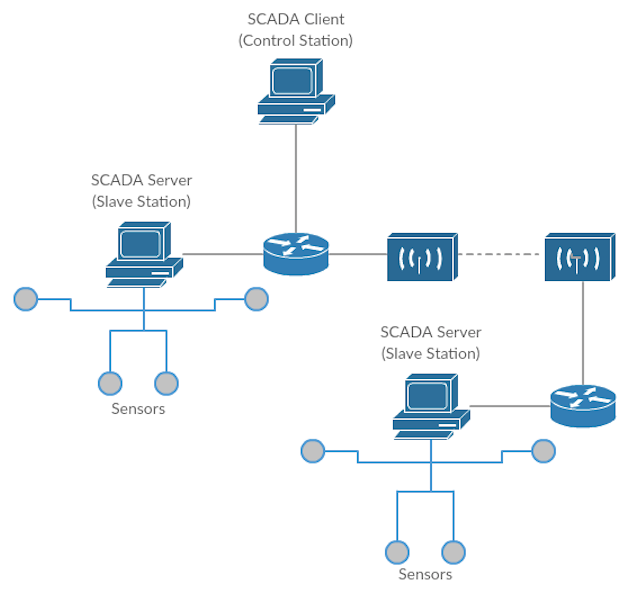
\includegraphics{scada}}
    \caption{Topológia SCADA systému}
\label{scada}
\end{figure}
Systémy slúžia na vzdialenú kontrolu a zber údajov. Využívajú sa v nich tzv. inteligentné merače - IED (Intelligent Electronic Devices). Jednotlivé zariadenia sú prepojené a vzájomne komunikujú cez aplikačnú zbernicu (fieldbus). Taktiež sú pripojené k riadiacemu centru, ktoré ich vzdialene kontroluje a ovláda. Ukážka prepojenia je na obrázku \ref{Fieldbus}. Vzdialenosť riadiach staníc (master) a koncových zariadení (slave) môže byť od niekoľkých metrov po tisíce kilometrov. Každé zariadenie môže obsahovať niekoľko rôznych senzorov, analógový vstup/výstup senzora, systém na komunikáciu s riadiacim počítačom a zariadeniami, a programovú pamäť\cite{SCADA}. \par
\begin{figure}[h]
    \centering
    \scalebox{0.6}{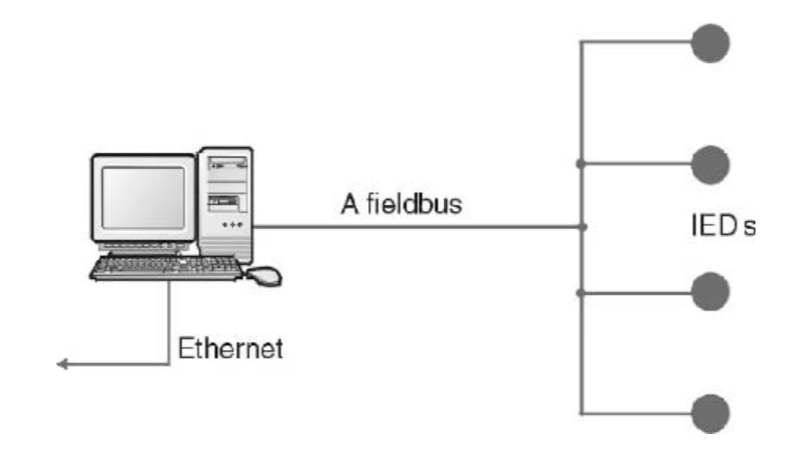
\includegraphics{Fieldbus}}
    \caption{Zapojenie zariadení v SCADA\cite{SCADA}}
\label{Fieldbus}
\end{figure}

\textbf{Výhody SCADA systémov sú:}
\begin{itemize}
\item Je potrebná minimálna kabeláž - oproti prvotným verziám SCADA systémov kedy sa nevyužívali IED zariadenia a každý senzor musel byť samostatne pripojený ku kontrolným staniciam
\item Prijímané dáta môžu obsahovať veľkú škálu informácií - seriové čísla, čísla modelu, informácie o inštalácií zariadenia (kedy bolo nainštalované a kým)
\item Zariadenia sú jednoduché na inštaláciu, prípadne výmenu
\item Celý systém potrebuje málo fyzického priestoru - jednotlivé koncové zariadenia sú relatívne malé
\end{itemize}
\textbf{Nevýhody sú:}
\begin{itemize}
\item Využívanie sofistikovanejších systémov je náročnejšie a vyžaduje lepšie vyškolený a kvalifikovaný personál
\item Ceny senzorov sú vyššie
\item Zariadenia sú závislé na komunikačnom systéme - je nutné aby podporovali rovnaký komunikačný protokol
\item Postupný prechod systémov nad IP vrstvu znižuje ich bezpečnosť\cite{SCADA}
\end{itemize}
\subsection{Komunikačné protokoly}
\tab Aby mohli medzi sebou koncové zariadenia a riadiaca stanica komunikovať, musia podporovať rovnaký spôsob komunikácie. Na to slúžia rôzne štandardizované protokoly, ktoré takúto komunikáciu popisujú. V tejto práci sa budem venovať dvom z nich. Konkrétne to sú protokoly IEC 60870-5-104 a DLMS/COSEM.
\subsubsection{IEC 60870-5-104}
\tab Protokol IEC 60870-5-104 je časť protokolu IEC 60870-5. IEC 60870-5 je komunikačný protokol a je súčasťou protokolu IEC 60870, ktorý je určený pre systémy diaľkového riadenia. IEC 60870-5 špecifikuje prenosové protokoly pre diaľkové ovládanie zariadení, ktoré slúžia k prenosu dát a riadeniu geograficky vzdialených procesov. Pozostáva z niekoľkých častí, z ktorých nás najviac zaujíma IEC 60870-5-104. Protokol IEC 60870-5-104 špecifikuje sieťový prístup pre IEC 60870-5-101. Protokol IEC 60870-5-101 je spoločná norma pre základné úlohy diaľkového ovládania. Jeho cieľom je zaistiť vzájomnú spoluprácu medzi jednotlivými (kompatibilnými) zariadeniami pre diaľkové riadenie. Tzn. že IEC 60870-5-101 špecifikuje mechanizmy prenosu a IEC 60870-5-104 stanovuje ich použitie v bežných komunikačných sieťach\cite{SCADA}\cite{Pekarek}.\par
Protokol IEC 60870-5-104 je umiestnený na aplikačnej vrstve modelu ISO/OSI. Špecifikácia IEC 60870-5-104 kombinuje aplikačnú časť protokolu IEC 60870-5-101 a prenosové funkcie poskytované TCP/IP. Protokol poskytuje funkcie pre prenos dat aplikačným funkciám užívateľského procesu. Prenášaná správa je vo formáte APDU (Application Protocol Data Unit). Je to tzv. aplikačná jednotka, ktorá pozostáva z dvoch častí - APCI (Application Protocol Control Information) a ASDU (Application Service Data Unit). APCI je záhlavie aplikačnej jednotky, ktoré určuje jej dĺžku, typ, sekvenčné čísla a pod. ASDU sú samotné prenášané dáta, tj. príkazy posielané medzi klientom a serverom. APDU správa môže mať pevnú alebo variabilnú dĺžku. Správa s pevnou dĺžkou neobsahuje ASDU časť. Formát rámca je ukázaný na obrázku \ref{APDU}.
\begin{figure}[h]
    \centering
    \scalebox{0.35}{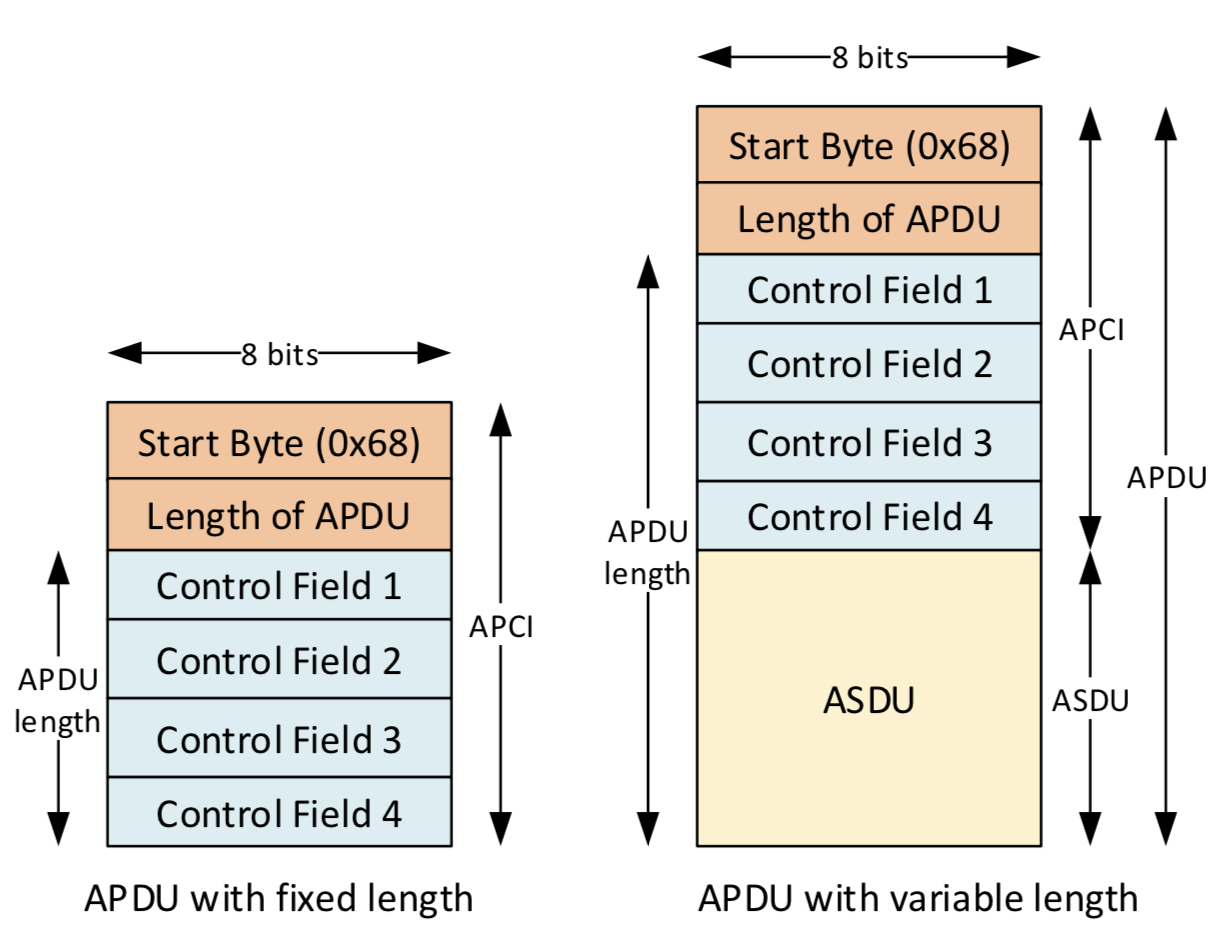
\includegraphics{APDU}}
    \caption{Formát APDU rámca\cite{iec}}
\label{APDU}
\end{figure}
Formát je určený poslednými dvoma bitmi prvého kontrolného poľa APCI časti (CF1). Štandard definuje tri typy rámcov, viď obrázok \ref{FrameFormat}.
\begin{figure}[h]
    \centering
    \scalebox{0.35}{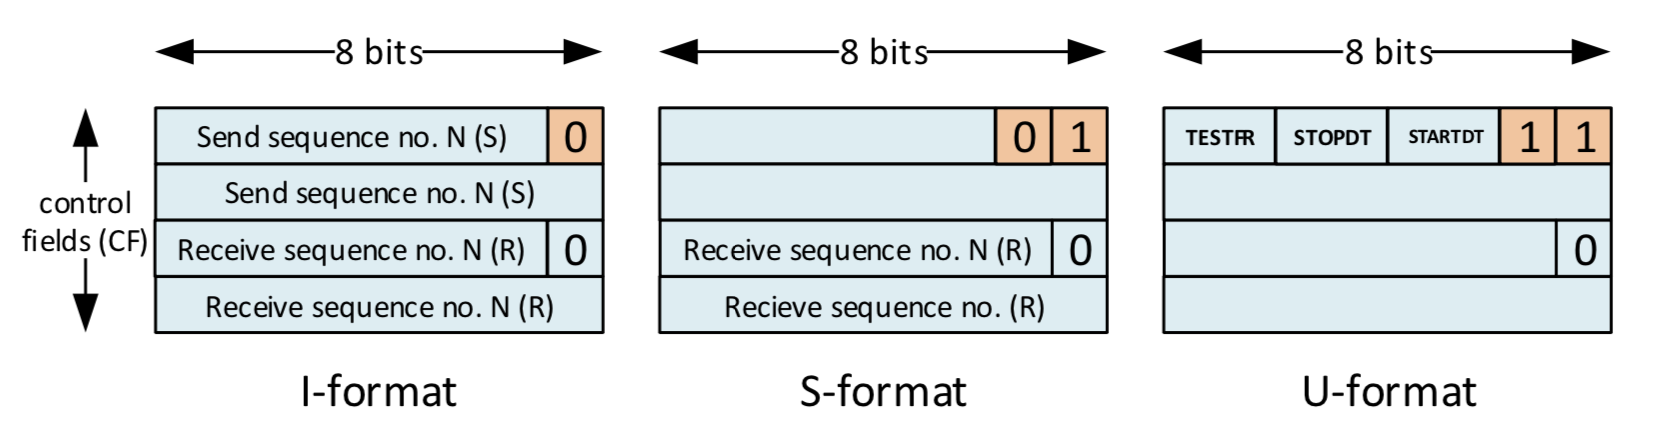
\includegraphics{FrameFormat}}
    \caption{Typy rámcov APDU\cite{iec}}
\label{FrameFormat}
\end{figure}
\begin{itemize}
\item I formát - je určený k bežnému prenosu dát medzi aplikačnými funkciami
\item S formát - je používaný pre dohľad nad prebiehajúcou komunikáciou
\item U formát - je určený k riadeniu samotnej komunikácie
\end{itemize}
\par
APCI vždy začína "štart bytom" s hodnotou 0x68. Za ňou nasleduje 8-bitové APDU a štyri 8-bitové kontrolné polia (CF). \par 
ASDU pozostáva z dvoch hlavných častí - identifikátor datovej jednotky (má vždy pevnú dĺžku šesť bytov) a dáta samotné, ktoré môžu pozostávať z jedného, alebo viacerých objektov. Identifikátor datovej jednotky definuje špecifický typ dát, poskytuje adresovanie na identifikáciu špecifickej identity dát a obsahuje dodatočné informácie ako napr. dôvod prenosu. Každé ASDU môže preniesť najviac 127 objektov. Na obrázku \ref{ASDU} je ukážka formátu ASDU\cite{iec}.
\begin{figure}[h]
    \centering
    \scalebox{0.4}{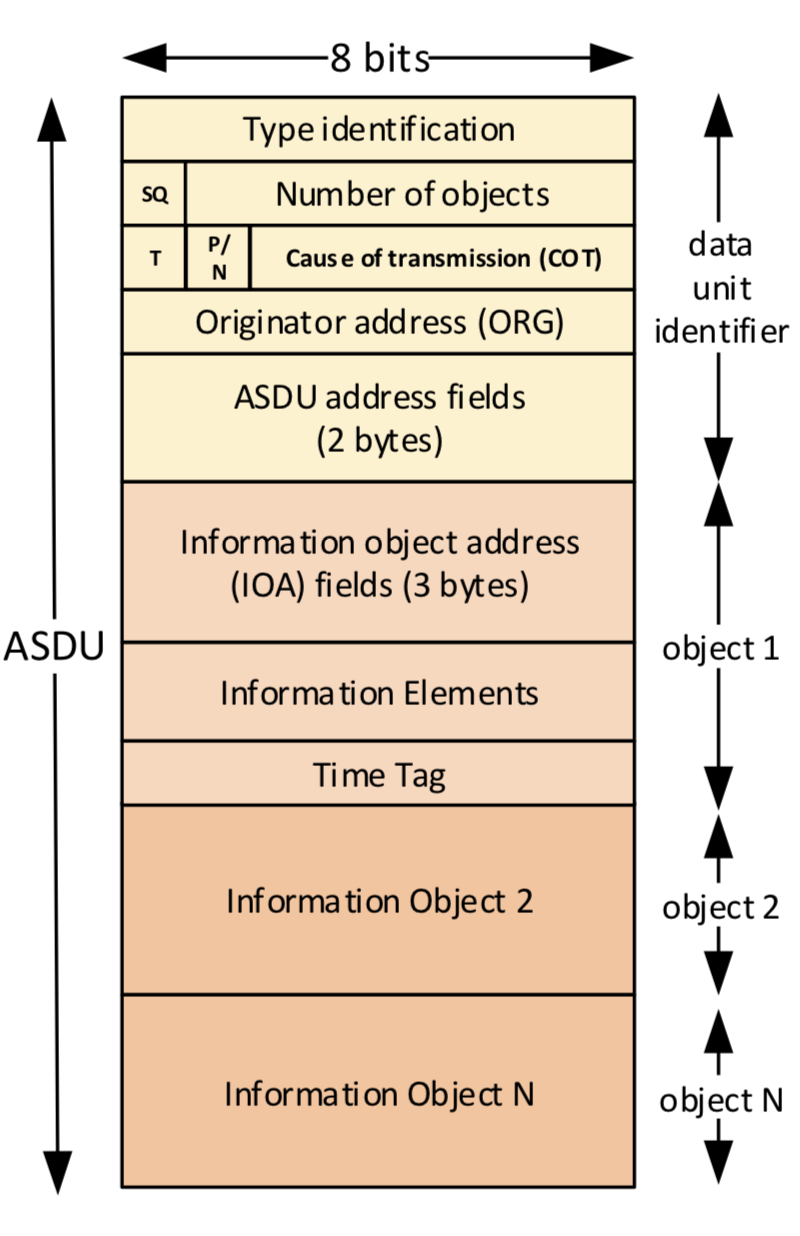
\includegraphics{ASDU}}
    \caption{Formát ASDU\cite{iec}}
\label{ASDU}
\end{figure}
\par
Riadenie prebieha pomocou niekoľkých príkazov - {\tt TESTFR}, {\tt STARTDT} a {\tt STOPDT}. {\tt STARDT} a {\tt STOPDT} sú príkazy používané riadiacimi stanicami na riadenie datového prenosu z riadenej stanice. Keď započne komunikácia, prenos dát nie je ešte povolený. Riadiaca stanica musí povoliť datový prenos odoslaním príkazu {\tt STARTDT act} (activate). Riadená stanica odpovie príkazom {\tt STARTDT con} (confirm). Ak nie je príkaz {\tt STARTDT} potvrdený, riadiaca stanica automaticky ukončí spojenie. Príkaz {\tt STARTDT} posiela iba riadiaca stanica a je odoslaný iba raz, po prvotnej inicializácií spojenia. Po povolení prenosu dát prebieha ľubovolná komunikácia medzi riadiacou a riadenou stanicou. Spojenie sa ukončuje príkazom {\tt STOPDT}.\par
Komunikácia vždy pozostáva medzi riadiacim (master) a riadeným (slave) systémom. Riadiaci systém inicializuje spojenie, začína a ukončuje výmenu aplikačných dát. Ukončenie komunikácie môže iniciovať riadiaca, ale aj riadená stanica. Riadená stanica (server) načúva na porte 2404 na príkazy od riadiacej stanice (klienta). Riadiaca stanica môže naraz komunikovať s viacerými riadenými stanicami\cite{iec}\cite{Pekarek}.
\subsubsection{DLMS/COSEM}
\tab Protokol DLMS/COSEM je, podobne ako protokol IEC 60870, súbor štandardov pre výmenu údajov o spotrebe v energetike. Protokol pozostáva z niekoľkých častí, pričom každá špecifikuje určitú časť problematiky, ktorú protokol rieši. Prvá časť, DLMS (Device Language Message Specification) je špecifikácia aplikačnej vrstvynezávislá od nižších vrstiev, vytvorená na podporu prenosu zpráv do a z vzdialených (energetických) zariadení. Cieľom je poskytnúť interoperabilné prostredie pre výmenu dát. Špecifikácia podporuje funkcie na vzdialené čítanie a nastavovanie hodnôt pre všetky odvetvia energetiky (elektrárne, vodárne, teplárne, atp.). DLMS je používané na popis rozhrania tried jednotlivých objektov spolu s ich atribútmi. Špecifikácia je podobná protokolu IEC 62056, ten je ale zameraný na meranie spotreby elektrickej energie na rozdiel od DLMS, ktorý je použiteľný na všetky energetické odvetvia. Druhá časť protokolu, COSEM (Companion Specification for Energy Metering) je rozhranie modelu komunikujúceho zariadenia na meranie energetickej spotreby, ktoré poskytuje pohľad na funkčnosť dostupnú cez komunikačné rozhranie. Poskytuje taktiež sémantiku na aplikáciu jednotlivých meraní. COSEM model je založený na objektovo-orientovanom prístupe. Instancia COSEM rozhrania sa nazýva {\tt COSEM interface object}. Sada jednotlivých objektov v logických zariadeniach fyzického zariadenia modeluje funkcionalitu meracích zariadení rovnako ako je to možné vidieť v jeho komunikačnom rozhraní\cite{dlmscosem}. \par
Model reprezentuje meracie zariadenie ako server využívaný aplikáciami klienta. Aplikácie slúžia na získavanie dát, poskytovanie riadiacich informácií a spušťanie funkcií objektu pomocou riadeného prístupu k jeho atribútom a špecifickým metódam jednotlivých typov objektov. \par
\begin{figure}[H]
    \centering
    \scalebox{0.3}{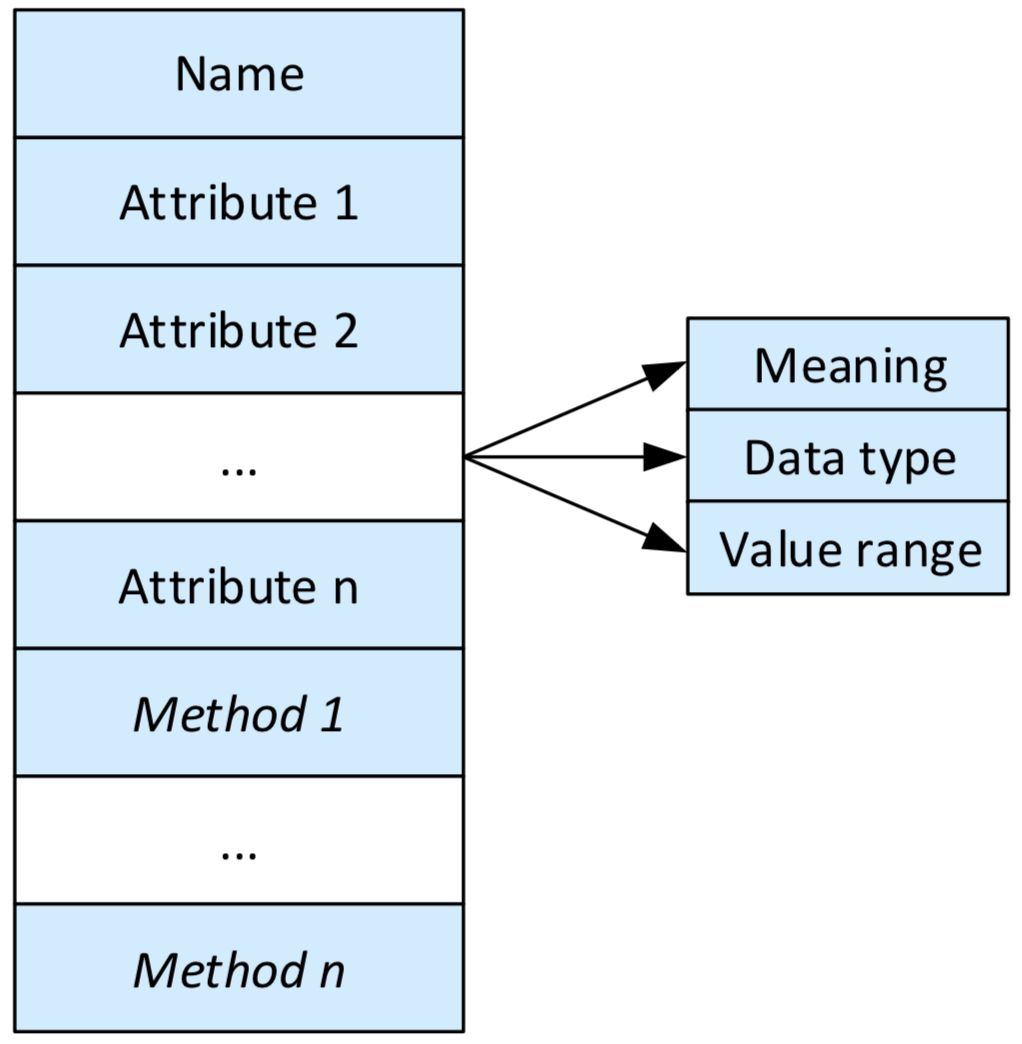
\includegraphics{dlmsattribute}}
    \caption{COSEM objekt\cite{dlmscosem}}
\label{dlmsattribute}
\end{figure}
COSEM modeluje fyzické zariadenie ako súbor logických zariadení, pričom každé má svoj jednoznačný identifikátor. Identifikátor určuje typ (funkcionalitu) daného zariadenia. Každé zariadenie môže byť jednoznačne identifikované pomocou jeho logického mena (OBIS kódom). Ide o šesť 8-bitových číslic. Informácie obsiahnuté v jednotlivých logických zariadeniach sú modelované objektami rozhrania. Objekty rozhrania sú špecifické pre danú doménu merania spolu s ich atribútmi a metódami. V atribútoch sú usporiadané informácie, ktoré daný objekt uchováva. Vlastnosti objektu sú určené pomocou hodnôt atribútov. Každý atribút pozostáva z typu, hodnoty a určenia. Ukážka objektu je na obrázku \ref{dlmsattribute}. \par
Prvý atribút každého objektu je jeho logické meno, ktoré slúži na identifikáciu objektu. Objekty, ktoré majú rovnakú charakteristiku sú generalizované a identifikované pomocou ID ich triedy (class\_id). Vzťah medzi šablónami a rozhraniami tried je ukázaný na obrázku \ref{dlmsobject}. Štandard protokolu definuje približne 70 rozhraní tried pričom každé je určené jeho menom, ID triedy a verziou.
\begin{figure}[H]
    \centering
    \scalebox{0.4}{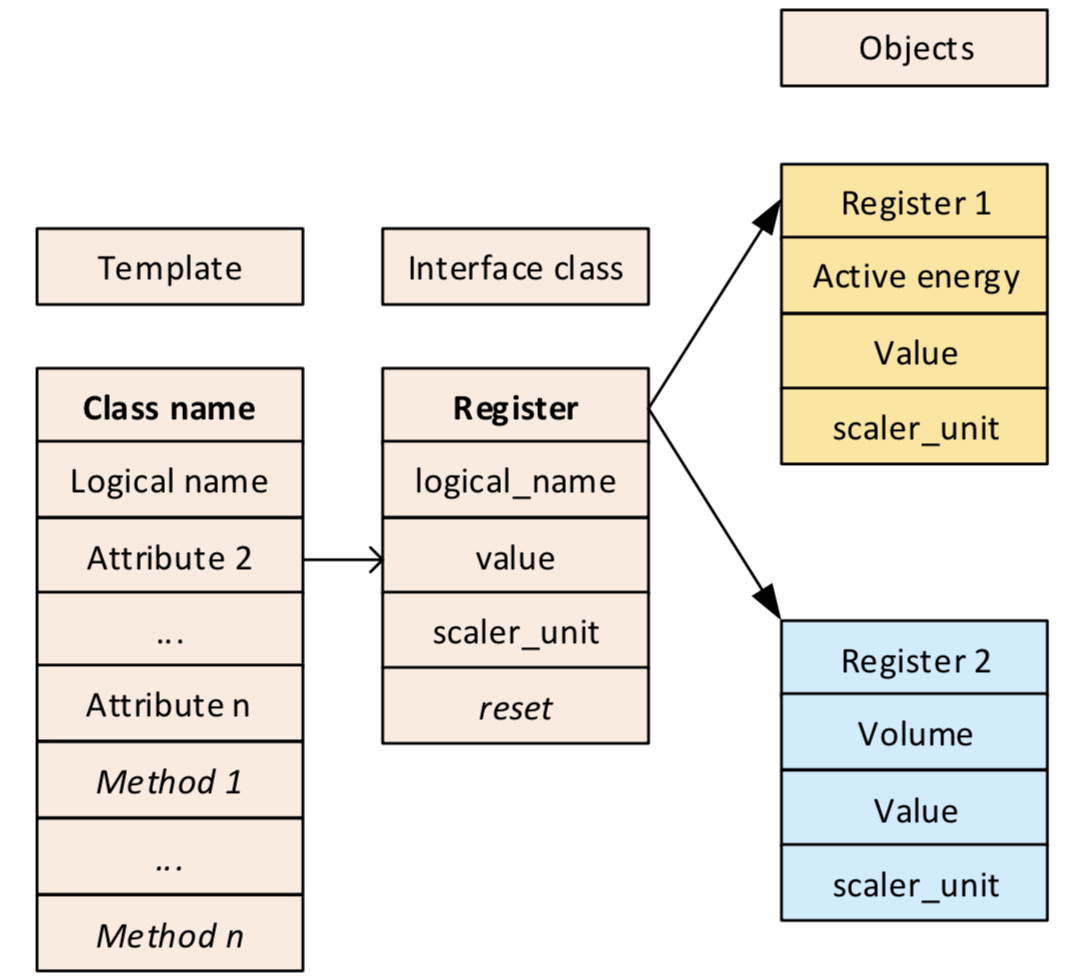
\includegraphics{dlmsobject}}
    \caption{Šablóny a rozhrania tried\cite{dlmscosem}}
\label{dlmsobject}
\end{figure}
Jednotlivé metódy umožňujú identifikáciu, vyhľadávanie a interpretáciu informácií uchovávaných v objektoch meracích zariadení\cite{dlmscosem}\cite{Horych}. \par
\begin{figure}[H]
    \centering
    \scalebox{0.6}{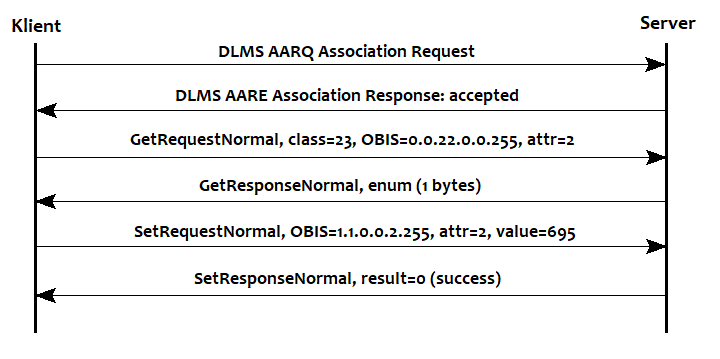
\includegraphics{comm.png}}
    \caption{Komunikácia protokolu DLMS/COSEM}
\label{dlmscom}
\end{figure}
Na obrázku \ref{dlmscom} je ukážka komunikácie protokolu DLMS/COSEM medzi klientom a serverom. Ukážka obsahuje niekoľko bežných príkazov. Ako prvé nnačítanie informácií o jednotlivých pripojených meračoch (Association Request/Response), tento príkaz je vždy zasielaný ako prvý na začiatku komunikácie. Druhá je žiadosť o navrátenie hodnoty druhého atribútu objektu s OBIS kódom 0.0.22.0.0.255. Ide o hodnotu prenosovej rýchlosti (baudrate) objektu typu {\tt IecHdlcSetup}. Nakoniec je zaslaný príkaz na nastavenie druhého atribútu objektu s OBIS kódom 1.1.0.0.2.255. Je to atribút nesúci údaje o spotrebe v objekte typu {\tt Data}. \par
Dáta prenášané protokolom DLMS/COSEM sú väčšinou zapúzdrené do tzv. HDLC rámca definovaného štandardom ISO/IEC 13239\cite{dlmscosem}. Štandard používa formát HDLC rámca typu 3, ukážka je na obrázku \ref{hdlc_frame}.
\begin{figure}[H]
    \centering
    \scalebox{0.6}{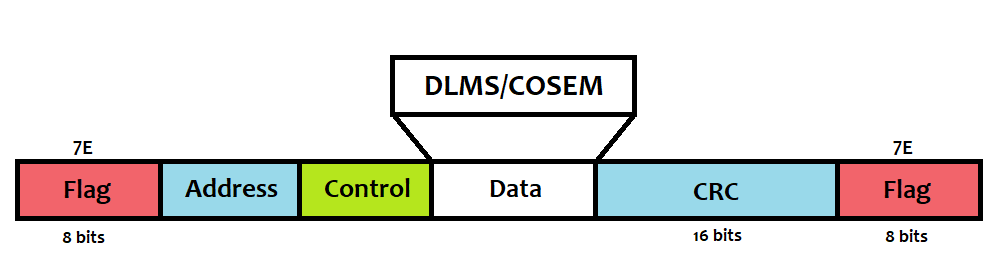
\includegraphics{hdlc_frame.png}}
    \caption{HDLC rámec}
\label{hdlc_frame}
\end{figure} \par
Rámec neobsahuje informačné pole, kontrolnú sekvenciu hlavičky (HCS) iba kontrolnú sekvenciu rámca. Prvé štyri bity slúžia na identifikáciu HDLC rámca. Pre DLMS je to 1010 (0xA). Kontrolné pole (CTRL) označuje typ príkazu alebo odpovede a obsahuje patričné sekvenčné číslo. Ukážka kontrolného poľa je na obrázku \ref{ctrl}.
\begin{figure}[H]
    \centering
    \scalebox{0.55}{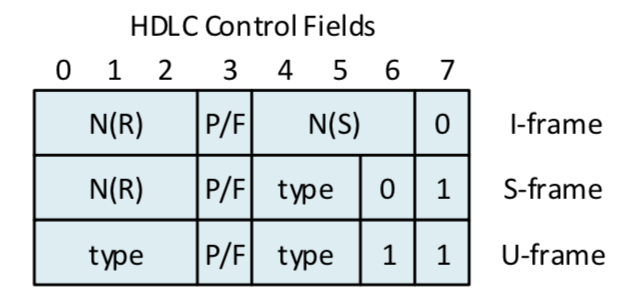
\includegraphics{ctrl}}
    \caption{Kontrolné pole HDLC rámca\cite{dlmscosem}}
\label{ctrl}
\end{figure} \par
Sú tri typy rámcov:
\begin{itemize}
\item I formát - informačný (information), prenáša užívateľské dáta zo sieťovej vrstvy 
\item S formát - kontrolný (supervisory), je používaný na kontrolu datového toku a chýb. Neobsahuje informačné polia. Používajú sa tri typy kontrolného rámca:
\begin{itemize}
\item 00: Pripravený na prijímanie, RR (Receive ready)
\item 01: Prijímanie, nie čítanie, RNR (Receive not read)
\item 10: Zamietnuté, REJ (Reject)
\item 11: Selektívne domietnutie, SREJ (Selective reject)
\end{itemize}
\item U formát - nečíslovaný (unnumbered) je používaný na správu odkazov (nastavenie režimu, zotavenie) a môže byť tiež použitý na prenos užívatľských dát
\end{itemize} \par
Pre DLMS/COSEM je potrebné parsovanie rámcov na identifikáciu vonkajšieho zapúzdrenia. HDLC môže byť identifikované začiatočným a koncovým príznakom (flag), ktorý má hodnotu 0x7e\cite{dlmscosem}.












  \chapter{Emulátory prevádzky SCADA systémov}
\label{porovnanie}
\tab V tejto kapitole uvediem základný prehľad a porovnanie bežne používanych monitorovacích a emulačných nástrojov pre protokoly IEC 60870-5-104 a IEC 60870-5-104. Programy, ktorým sa budem venovať, slúžia nielen na~monitorovanie komunikácie reálnych IEC 60870-5-104 a DLMS/COSEM meracích zariadení, ale aj na ich emuláciu. Popis inštalácie jednotlivých programov je uvedený v prílohe \ref{Ako}.
\section{IEC 60870-5-104 - DLMS/COSEM}
\subsection{DMLS Director}
\textbf{Výrobca:} Firma GuruX Ltd. je fínska spoločnosť špecializujúca sa na protokol DLMS využívaný v inteligentných meračoch\footnote{GuruX Ltd. \url{http://www.gurux.fi} [Online: Október 2017]}. Firma poskytuje produkty pre automatické zaznamenávanie hodnôt z meracích zariadení a umožnuje tým vytvorenie vlastných AMR systémov (systémov pre automatickú správu meracích zariadení). \par
\noindent \textbf{Popis produktu:} DLMS Director je open source software navrhnutý na DLMS komunikáciu a smart metering s DLMS/COSEM zariadeniami. \par 
\noindent \textbf{Protokoly:} Program DLMS Director pokrýva niekoľko komunikačných štandardov. Je zameraný na čítanie údajov a rozposielanie príkazov. Jednotlivé protokoly sú: 
\begin{itemize}
\item IEC 62056-21 Priama lokálna výmena dát
\item IEC 62056-42 Služby a procedúry pre asynchrónnu spojovú výmenu dát na fyzickej vrstve
\item IEC 62056-46 Linková vrstva využívajúca HDLC protokol
\item IEC 62056-47 COSEM transportná vrstva pre IPv4
\item IEC 62056-53 COSEM aplikačná vrstva
\item IEC 62056-61 OBIS systém na identifikáciu objektov
\item IEC 62056-62 Interface
\end{itemize} \par
\noindent \textbf{Zariadenia:} Program je schopný pracovať iba s reálnymi fyzickými zariadeniami, prípadne so zariadeniami emulovanými iným programom. Sám ich však emulovať nedokáže. So zariadeniami môže byť pripojený cez TCP/IP spojenie, terminál, alebo cez sériovú linku. \par
\noindent \textbf{Typ:} DLMS Director je open source software, ktorý je voľne dostupný na stránkach výrobcu. Zdrojové kódy sú taktiež voľne dotupné v pratričnom github repozitári\footnote{DLMS Director - zdrojové kódy \url{https://github.com/Gurux/GXDLMSDirector} [Online: Október 2017]}. \par
\noindent \textbf{Platforma:} Program je vytvorený pre OS Windows. Na iných platformách s ním nie je možné pracovať. \par
\noindent \textbf{Prípadová štúdia:} Program samotný slúži ako jedna klientská stanica umožňujúca pripojenie niekoľkých meracích zariadení. Pri pridávaní nového zariadenia je možnosť nastavenia jednotlivých parametrov spolu s preddefinovanými hodnotami. Ukážka pridania nového zariadenia je na obrázku \ref{DLMSConf}. 
\begin{figure}[h]
    \centering
    \scalebox{0.8}{\includegraphics{DLMSdirectorConf.png}}
    \caption{Konfigurácia nového zariadenia v programe DLMS Director}
\label{DLMSConf}
\end{figure}
Odkaz na popis konfigurácie rôznych zariadení je medzi prílohami, časť \ref{Ako_DLMS}. Po pripojení k serveru zobrazí program zoznam všetkých objektov, ktoré server obsahuje. Objekty sú rozdelené do množín podľa ich typu, napr. {\tt Data, Register, Clock, MacAddress Setup}. Ukážka je na obrázku \ref{DLMS_List}.
\begin{figure}[h]
    \centering
    \scalebox{0.55}{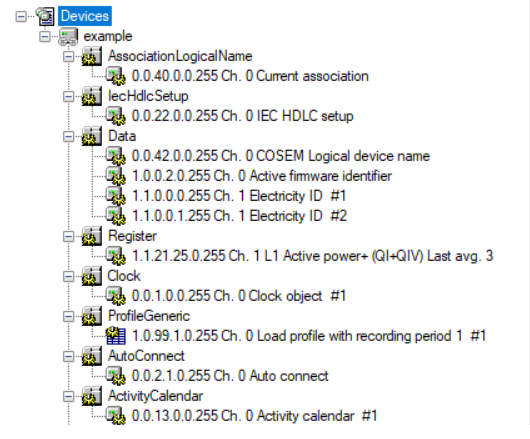
\includegraphics{DLMS_List.png}}
    \caption{Zoznam pripojených objektov}
\label{DLMS_List}
\end{figure}
Je možné čítať hodnoty atribútov jednotlivých objektov, avšak iba všetkých hodnôt naraz. Nie je možné odoslať samostatný príkaz na prečítanie napríklad logického mena objektu. Je tiež možné prečítať hodnoty celej skupiny objektov v jednom príkaze, ale iba v rámci jedného typu. Napríklad hodnoty objektov typu {\tt Data}. \par
Pri testovaní bola použitá knižnica v jazyku C++, ktorú poskytuje spoločnosť GuruX. Knižnica je voľne k dispozícií v Github repozitári\footnote{DLMS knižnica - Github \url{https://github.com/Gurux/Gurux.DLMS.cpp} [Online: Marec 2018]} a umožňuje vytvorenie vlastných aplikácií pre DLMS. Spolu s knižnicou sú k dispozícií vzorové programy pre klienta a server. Programy sú vytvorené pre OS Linux. Návod na inštaláciu knižnice je medzi prílohami \ref{kniznica}. Vzorový program servera vytvorí pri spustení štyri rôzne DLMS servery:
\begin{itemize}
\item port 4060 - DLMS server využívajúci krátke mená (Short Names - SN)
\item port 4061 - DLMS server využívajúci logické mená (Logical Names - LN) 
\item port 4062 - DLMS server využívajúci krátke mená spolu s protokolom IEC 62056-47
\item port 4063 - DLMS server využívajúci logické mená spolu s protokolom IEC 62056-47
\end{itemize} \par
Samotné testovanie pozostávalo vo vytvorení spojenia medzi programom DLMS Director a vzorovým programom pre server. Program bol ale čiastočne upravený aby bol užívateľsky o niečo prívetivejší a aby podporoval väčšiu škálu možností. Po spustení sa vytvorí iba jeden server na porte 4060 využívajúci logické mena. Bola pridaná možnosť hodnoty vzdialene meniť, nie iba čítať a bola pridaná možnosť využívať autentizáciu heslom typu {\tt low}. Zmenený program bol umiestnený na github repozitár\footnote{GitHub \url{https://github.com/janpristas/bakalarska-praca}}. Na jeho úspešnú kompiláciu a spustenie je potrebné mať nainštalovanú vyššie spomínanú knižnicu. \par
Vytvorenie spojenia a testovanie pozostávalo z niekoľkých krokov:
\begin{enumerate}
\item Bol spustený DLMS Director a program servera. Server nebolo nutné nijako ďalej konfigurovať. Bolo možné sa s ním priamo spojiť.
\item V DLMS Directore bolo potrebné nakonfigurovať server s ktorým sa ide program spojiť:
\begin{enumerate}
\item {\tt File} $\rightarrow$ {\tt Add Device}
\item Zvoliť meno pre server
\item Zvoliť výrobcu $\rightarrow$ {\tt Gurux}, 
\item Zvoliť autentizáciu $\rightarrow$ {\tt Low} a heslo $\rightarrow$ {\tt password} (nastavené v programe servera)
\item Nastaviť IP adresu servera a port 4060
\end{enumerate}
\item Po úspešnom nakonfigurovaní bolo možné vytvoriť spojenie so serverom. Spojenie inicializuje program DLMS Director. V ľavom paneli bolo potrebné rozkliknúť zoznam {\tt Devices} a kliknúť pravým tlačítkom na server, následne na {\tt Connect}.
\item Po vytvorení spojenia sa zobrazil zoznam pripojených zariadení, z ktorých bolo možné čítať a zapisovať hodnoty, príkazy {\tt Read} a {\tt Write}.
\end{enumerate} \par
Testovaciu topológiu je možné vidieť na obrázku \ref{dlmstopology}.
\begin{figure}[h]
    \centering
    \scalebox{0.8}{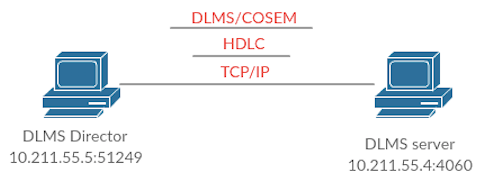
\includegraphics{dlms_topology}}
    \caption{Ukážka testovacej topológie pre program DLMS Director}
\label{dlmstopology}
\end{figure}
Testovací server obsahoval niekoľko rôznych objektov. Testovanie spočívalo v dotazovaní sa na hodnoty atribútov týchto objektov. Objekty boli napríklad typu {\tt Data, Clock, SapAssigment, ActivityCalendar}. Komunikácia bola zachytená pomocou nástroja Wireshark a bol vytvorený súbor DLMSDirector.pcap uložený v github repozitári. \footnote{GitHub \url{https://github.com/janpristas/bakalarska-praca}} \par
\noindent \textbf{Zhrnutie:} DLMS Director je dobre spracovaný program určený hlavne na čítanie údajov a riadenie meracích zariadení. Výhodou je, že je typu open source a možno s ním zdarma pracovať. Nevýhodou je chýbajúca možnosť emulovania koncových zariadení a tým aj prevádzky samotnej.

\subsection{XmlDemo}
\textbf{Výrobca:} iCube je švajčiarska softwarová firma zaoberajúca sa, podobne ako vyššie spomínaná firma GuruX, vývojom softwaru pre komunikačný protokol DLMS\footnote{iCube \url{https://www.icube.ch/index.html} [Online: Október 2017]}. Firma ponúka DLMS vývojové komunikačné balíky pre jazyky C++, C\# a Java, zjednodušujúce implementáciu DLMS/COSEM klientských aplikácií. Vo variante C++ sú jednotlivé komponenty implementované ako DLL, v C\# a Java variantách sú implementované ako triedy. Jednotlivé balíky ale nebudem bližšie rozoberať. \par
\noindent \textbf{Popis produktu:} XmlDemo je jednoduchý DLMS "čítač"\ hodnôt uložených v DLMS/COSEM meracích zariadeniach. Implementácia využíva vyššie spomenuté DLMS balíky, konkrétne komponenty {\tt xmlpdu} na výstup vo formáte xml, {\tt ezhdlc} pri vyžití HDLC spojenia a {\tt wrapper} pri spojení cez TCP/IP. Program XmlDemo je v úlohe klienta, ktorý zasiela žiadosti serveru (zariadeniam) a prijíma odpovede. Napríklad, klient pošle žiadosť {\tt read the object 1.0.1.8.0.255} a server odpovie {\tt 1789.8 kWh}. \par
\noindent \textbf{Protokoly:} Program je vytvorený na komunikáciu so zariadeniami pomocou protokolu DLMS/COSEM. \par
\noindent \textbf{Zariadenia:} Program je schopný pracovať iba s reálnymi fyzickými zariadeniami, prípadne so zariadeniami emulovanými iným programom. Sám ich emulovať nedokáže. Podporuje komunikáciu medzi zariadeniami a aplikáciou cez TCP/IP a HDLC. \par
\noindent \textbf{Typ:} XmlDemo je zdarma poskytovaný program spoločnosťou iCube, nakoľko sa jedná o ukážku programu vytvoreného vo vyššie spomínaných vývojových balíkoch. \par
\noindent \textbf{Platforma:} Obdobne ako predchádzajúci program je aj XmlDemo prispôsobený iba na OS Windows. Na obrázku \ref{XmlDemo} je ukážka užívateľského rozhrania. Spôsob prijímania správ a logovací záznam vo formáte xml je na obrázku \ref{XmlDemo-term}. \par
\begin{figure}[h]
	\centering
    \scalebox{0.48}{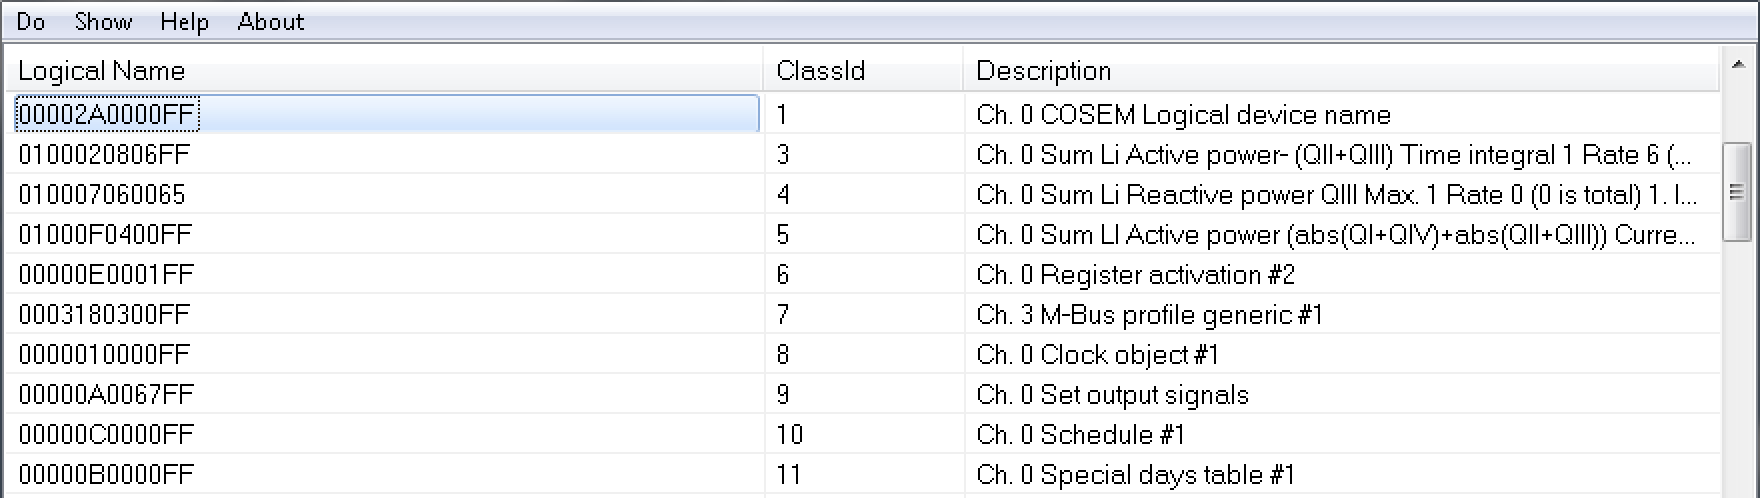
\includegraphics{XMLDemo}}
    \caption{Užívateľské rozhranie XmlDemo}
\label{XmlDemo}
\end{figure} \par

\begin{figure}[h]
    \centering
    \scalebox{0.6}{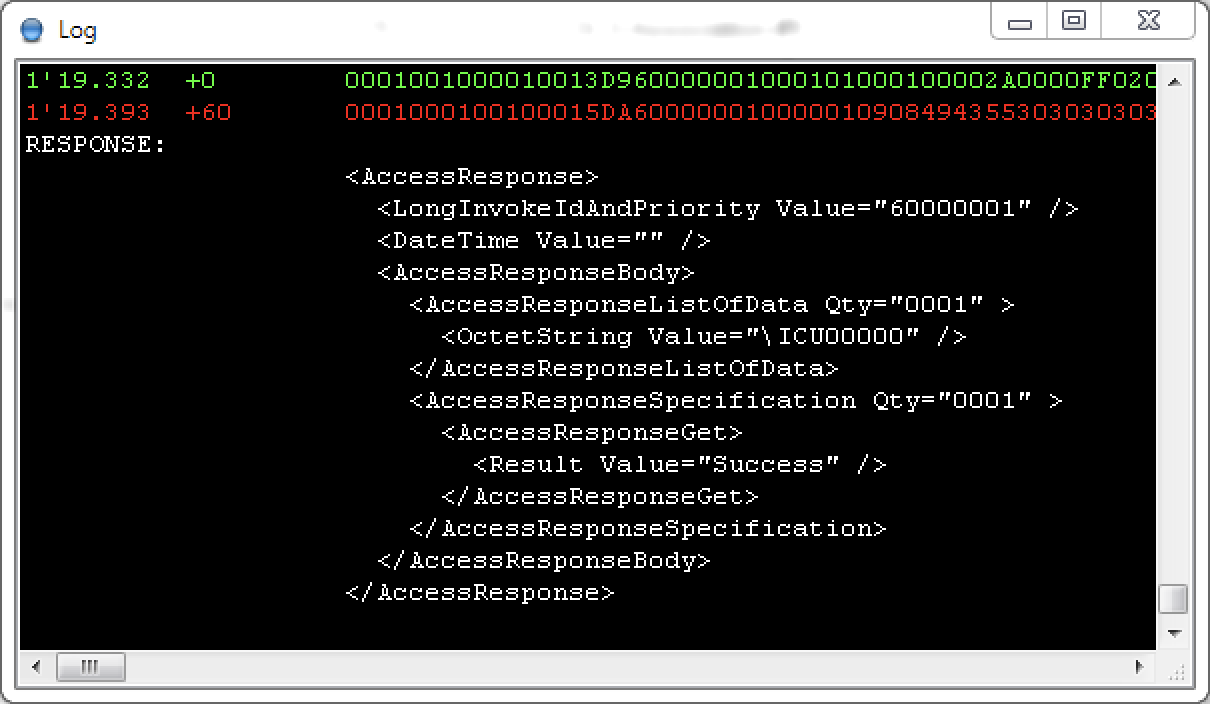
\includegraphics{XMLDemo-terminal}}
    \caption{Užívateľské rozhranie XmlDemo}
\label{XmlDemo-term}
\end{figure} \par
\noindent \textbf{Prípadová štúdia:} Čo sa topológie týka, program funguje ako vyššie popísaný DLMS Director. Program samotný slúži ako klientská stanica, ku ktorej je možné pripojiť jednotlivé monitorovacie zariadenia. \par
Pri testovaní bol použitý vzorový program pre server komunikujúci na porte 4063 využívajúc spojenie cez TcpUdp. Program XmlDemo síce umožňuje komunikáciu so serverom cez HDLC, avšak iba ak sú zariadenia prepojené cez sériovú linku. To som však nemal pri testovaní možnosť vyskúšať, nakoľko som nemal k dispozícií reálne fyzické zariadenie. \par
Vytvorenie spojenia medzi klientom a serverom opäť pozostávalo z niekoľkých krokov:
\begin{enumerate}
\item Bol spustený program XmlDemo a pôvodný vzorový program servera, neobsahújúci nijaké zmeny. 
\item Bolo potrebné nakonfigurovať program XmlDemo:
\begin{enumerate}
\item {\tt Show} $\rightarrow$ {\tt Settings}
\item {\tt Select TCP profile}
\item Nastaviť IP adresu servera a port 4063
\item Nastaviť referenčný model $\rightarrow$ {\tt LN}
\item Nastaviť timeout, obe hodnoty {\tt Connect} a {\tt Response} na prijateľné hodnoty v milisekundách, v našom prípade 1000
\item Nastaviť adresy pre klienta aj server, v našom prípade obe na 0
\end{enumerate}
\item Po nakonfigurovaní bolo možné vytvoriť spojenie. {\tt Do} $\rightarrow$ {\tt Connect} a {\tt Do} $\rightarrow$ {\tt Read object-list}.
\end{enumerate} \par
Testovacia topológia je obdobná ako pri testovaní programu DLMS Drector. Je možné ju vidieť na obrázku \ref{xmldemotopology}.
\begin{figure}[h]
    \centering
    \scalebox{0.8}{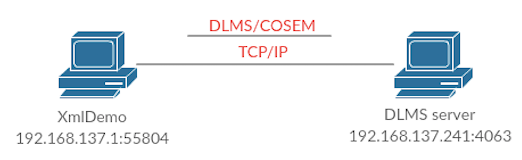
\includegraphics{xmldemo_topology}}
    \caption{Ukážka testovacej topológie pre program XmlDemo}
\label{xmldemotopology}
\end{figure}
 Po vytvorení spojenia medzi klientom a serverom, program (XmlDemo) automaticky zobrazí zoznam všetkých pripojených objektov. Objekty sú taktiež uložené do nového .txt súboru. Zoznam je zobrazený vo formáte - {\tt logické meno | id triedy | popis}. Zápis objektu vyzerá napríklad $\rightarrow$ {\tt 0000010000FF | 8 | Ch. 0 Clock object \#1}. Následne je možné z jednotlivých objektov čítať hodnoty atribútov. Je možné čítať hodnoty iba vybraných atribútov, na rozdiel od programu DLMS Director, ktorý umožňuje iba čítanie všetkých hodnôt daného objektu naraz. Po kliknutí na jednotlivé objekty sa zobrazí zoznam ich atribútov. Po kliknutí na jednotlivé atribúty sa prečíta ich hodnota. Testovanie prebiehalo obdobne ako pri programe DLMS Director. Komunikácia bola zachytená nástrojom Wireshark a bol vytvorený súbor XmlDemo.pcap uložený v github repozitári. \footnote{GitHub \url{https://github.com/janpristas/bakalarska-praca}} \par
\noindent \textbf{Zhrnutie:} Čo sa týka samotnej funkcionality, poskytuje program obdobné funkcie a možnosti ako program DLMS Director, avšak hlavnou nevýhodou je absencia komunikácie pomocou HDLC cez IP vrstvu. Je to možné iba na fyzickej vrstve. Na testovacie účely je preto vhodnejší program DLMS Director. XmlDemo taktiež ponúka o niečo horšie GUI, v ktorom sa nepracuje tak dobre a intuitívne ako v DLMS Directore.

\section{IEC 60870-5-104}
\subsection{WinPP104}
\textbf{Výrobca:} Firma Berthold Boeser Ingenieurbüro je nemecká spoločnosť, ktorá vyvíja a distribuje testovacie programy pre protokoly diaľkového riadenia\footnote{Berthold Boeser Ingenieurbüro \url{http://www.ppfink.de//} [Online: Október 2017]}. Jednotlivé protokoly sú: 
\begin{itemize}
\item IEC: 60870-5-101, 60870-5-102, 60870-5-103, 60870-5-104
\item AEG: GEADAT 81, GEATRANS F202, F203, F220, F202KC, SEAB 1-F/N, PMF234C
\item BBC: ZM20, I21
\item Landis\&Gyr: TELEGYR 800
\item Mauell: ME 8008, 8018 PDM
\item SAT: 1703 PCM
\item SEL: ZPC3600/SPC17
\item Siemens: SINAUT ST1, 4-FW, SINAUT 8-FW DPDM, SINAUT 8-FW PCM, FW 517/535/537, EFD 400, SAS/Z70
\end{itemize} \par
\noindent \textbf{Popis produktu:} WinPP104 je testovací a emulačný nástroj pracujúci nad protokolom IEC 60870-5-104. Okrem bežnej komunikácie tiež umožňuje odosielanie a prijímanie správ iba simulovať a tým sledovať rôzne faktory ako napr. oneskorenie príkazu. Výsledný záznam komunikácie sa dá exportovať do .csv súboru. Program rovnako umožňuje záznamy z .csv súborov aj nahrávať a následne ich spracovať. \par
\noindent \textbf{Protokoly:} Program je uspôsobený na komunikáciu výhradne nad protokolom IEC 60870-5-104. \par
\noindent \textbf{Zariadenia:} WinPP104 umožňuje sledovať reálne fyzické meracie zariadenia, ale aj vytvorenie vlastného klienta alebo servera pre simulačné účely. Prepojenie medzi zariadeniami je možné cez LAN alebo TCP/IP. \par
\begin{figure}[H]
    \centering
    \scalebox{0.35}{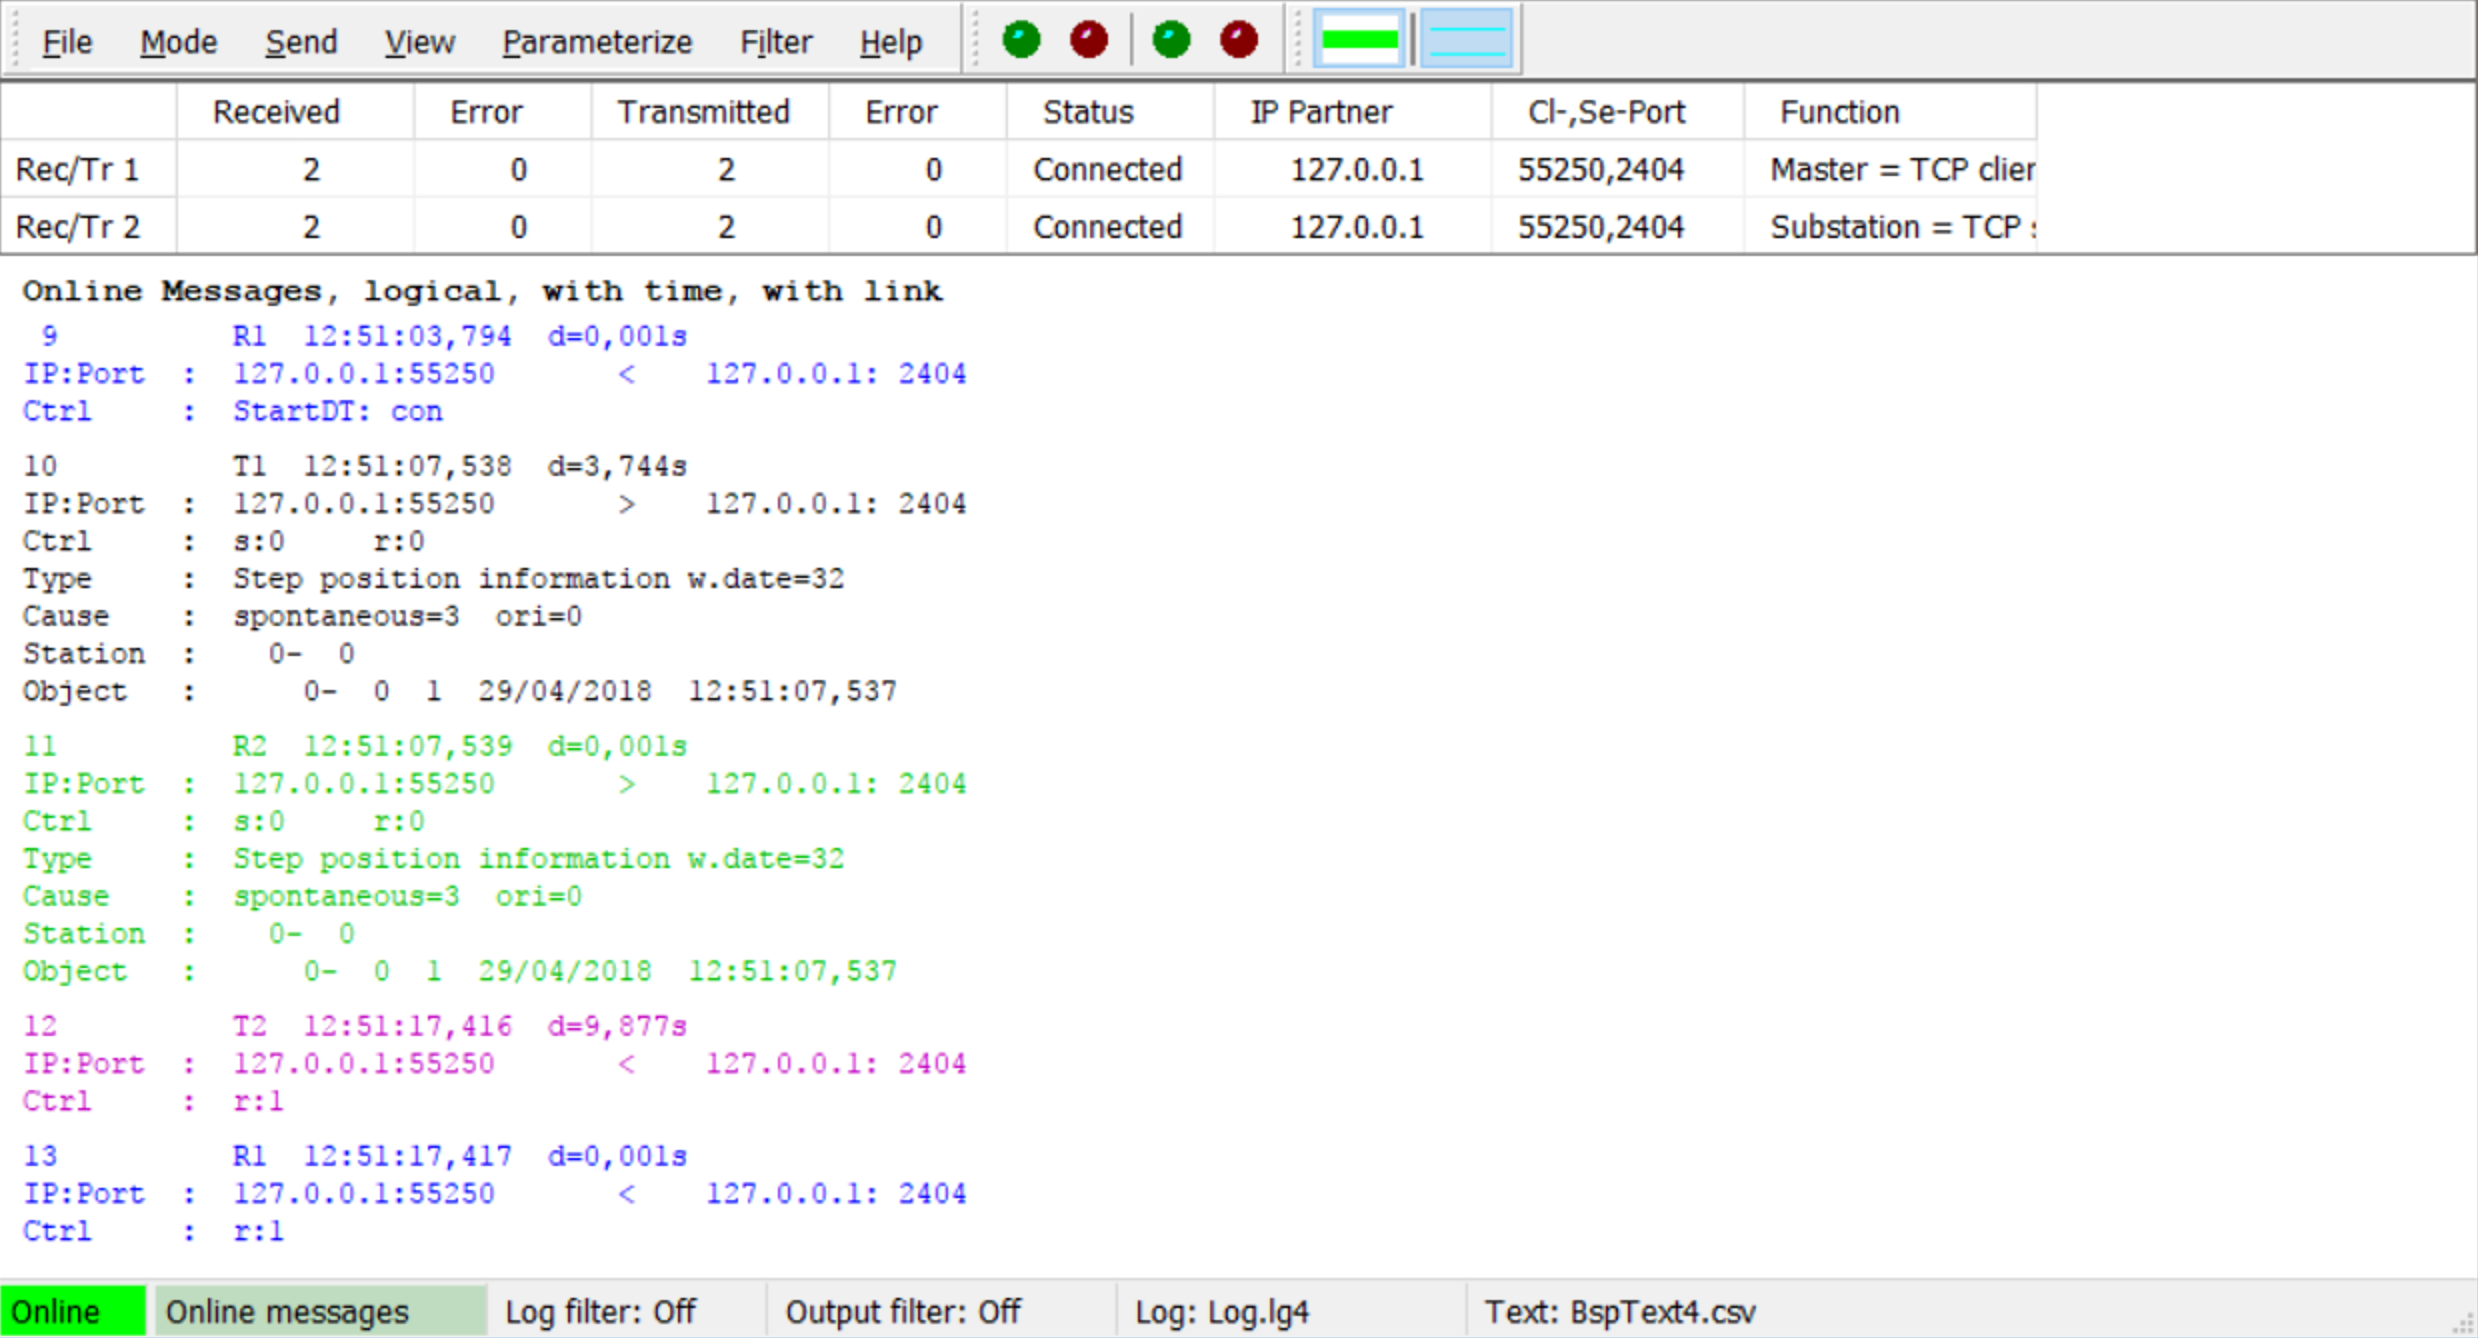
\includegraphics{WinPP104}}
    \caption{Užívateľské rozhranie WinPP104}
\label{WinPP104}
\end{figure}
\noindent \textbf{Typ:} Výrobca poskytuje zdarma demo verziu, ktorá má však určité obmedzenia. Pri každom spustení aplikácie je nutné si celý systém nanovo nastavovať, naše predošlé nastavenia nebudú uložené. Navyše je možné prijať a odoslať iba 20 správ, čo striktne zamedzí dlhodobému monitorovaniu systému. \par
\noindent \textbf{Platforma:} Program je vytvorený na platformu OS Windows. Na obrázku \ref{WinPP104} je ukážka užívateľského rozhrania programu WinPP104, konkrétne ide o ukážku pripojenia zariadení cez TCP/IP a o ich monitorovanie. \par
\noindent \textbf{Prípadová štúdia:} WinPP104 umožňuje v rámci jedného spustenia vytvorenie jednej stanice klienta a jednej stanice servera. Je ale možné program spustiť niekoľkokrát a emulovať niekoľko klient/server spojení. Pri vytváraní nového uzlu poskytuje program defaultné nastavenia, ktoré je možné vidieť na obrázku \ref{WinPP104Conf}.
\begin{figure}[h]
    \centering
    \scalebox{0.5}{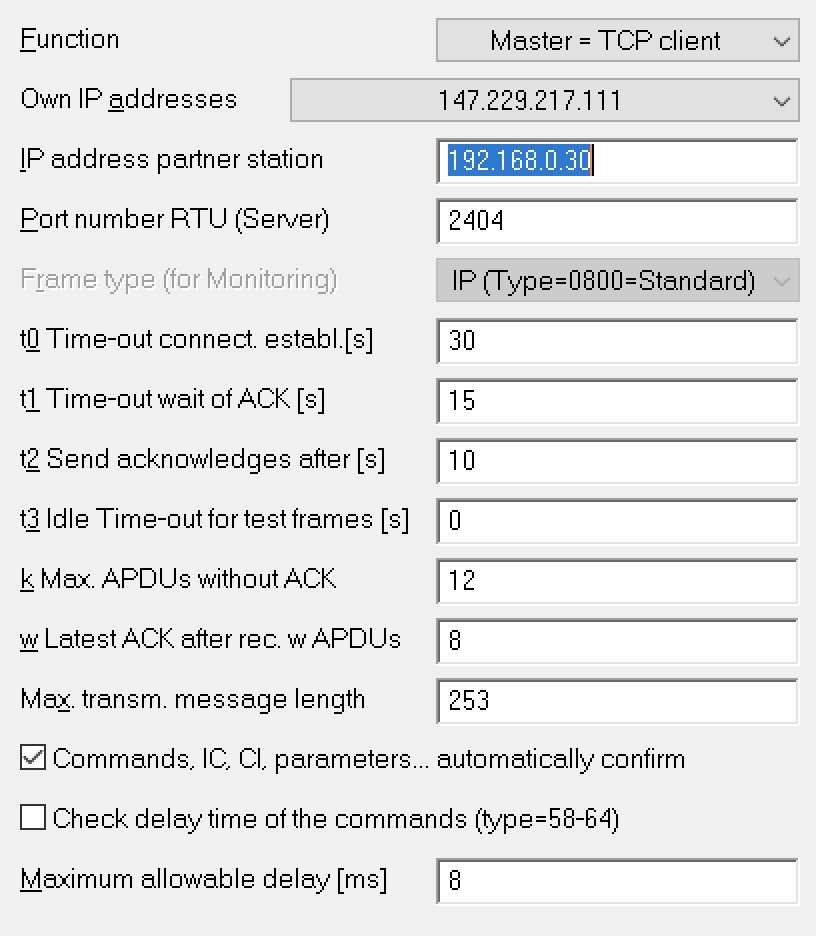
\includegraphics{WinPP104C}}
    \caption{Konfigurácia nového objektu}
\label{WinPP104Conf}
\end{figure} \par
Vytvorenie testovacieho prostredia pozostávalo z niekoľkých častí:
\begin{enumerate}
\item Spustenie programu WinPP104
\item Konfigurácia nového uzlu klienta:
\begin{enumerate}
\item {\tt Parameterize} $\rightarrow$ {\tt Receiver/Transmitter 1}
\item {\tt Function} = {\tt Master = TCP Client}
\item {\tt IP address partner station} = 127.0.0.1
\item {\tt Port number RTU (Server)} = 2404
\item Zvyšné parametre mali defaultné hodnoty
\item {\tt OK}
\end{enumerate}
\item Konfigurácia nového uzlu servera:
\begin{enumerate}
\item {\tt Parameterize} $\rightarrow$ {\tt Receiver/Transmitter 2}
\item {\tt Function} = {\tt Substation = TCP Server}
\item {\tt IP address partner station} = 127.0.0.1
\item {\tt Port number RTU (Server)} = 2404
\item Zvyšné parametre mali defaultné hodnoty
\item {\tt OK}
\end{enumerate}
\item {\tt Mode} $\rightarrow$ {\tt Online}, následné sa vytvorilo spojenie medzi jednotlivými uzlami a bolo možné zasielať príkazy
\end{enumerate}
Pri samotnej komunikácií poskytuje program 12 preddefinovaných správ a 12 zoznamov. Je možné ich dodatočne prekonfigurovať podľa potreby:
\begin{itemize}
\item {\tt Parameterize} $\rightarrow$ {\tt Messages} $\rightarrow$ 1,2,3,...
\item {\tt Parameterize} $\rightarrow$ {\tt Lists} $\rightarrow$ 1,2,3,...
\end{itemize}
Je možné nastaviť napr. typ správy, dôvod (cause) odoslania správy, zdrojovú, cieľovú adresu a pod. Ukážka konfigurácie správy je na obrázku \ref{WinPP104Mess}.
\begin{figure}[h]
    \centering
    \scalebox{0.5}{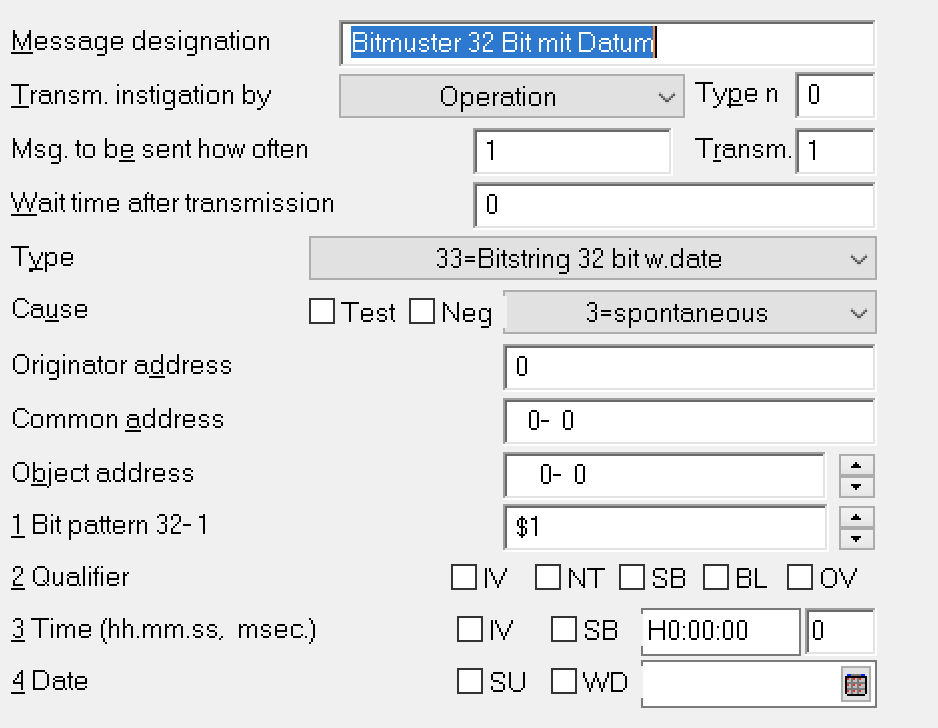
\includegraphics{WinPP104M}}
    \caption{Konfigurácia novej správy}
\label{WinPP104Mess}
\end{figure} \par
Zasielanie správ alebo zoznamov je možné cez {\tt Send} $\rightarrow$ {\tt Messages}/{\tt Lists} $\rightarrow$ 1,2,3,... \par
Testovanie pozostávalo vo vytvorení jednoduchej topológie a v zaslaní/prijatí niekoľkých preddefinovaných správ aby sa overilo, či komunikácia odpovedá štandardom protokolu IEC 60870-5-104. Ukážka testovacej topológie je na obrázku \ref{WinPP104-Topology}.
\begin{figure}[h]
    \centering
    \scalebox{0.8}{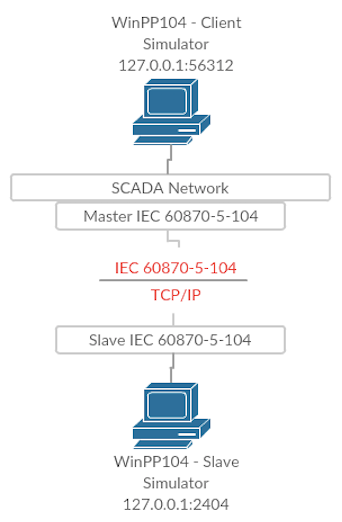
\includegraphics{WinPP104-Topology}}
    \caption{WinPP104 - Testovacia topológia}
\label{WinPP104-Topology}
\end{figure}
Program bol spustení na jednom zariadení a komunikácia bola zachytená nástrojom RawCap na rozhraní loopback. Z komunikácie bol vytvorený .pcap súbor WinPP104.pcap uložený v github repozitári \footnote{GitHub \url{https://github.com/janpristas/bakalarska-praca}}. Z následnej analýzy odchytených dát bolo overené, že komunikácia bola validná a odpovedala protokolu IEC 104.
\begin{figure}[H]
    \centering
    \scalebox{0.4}{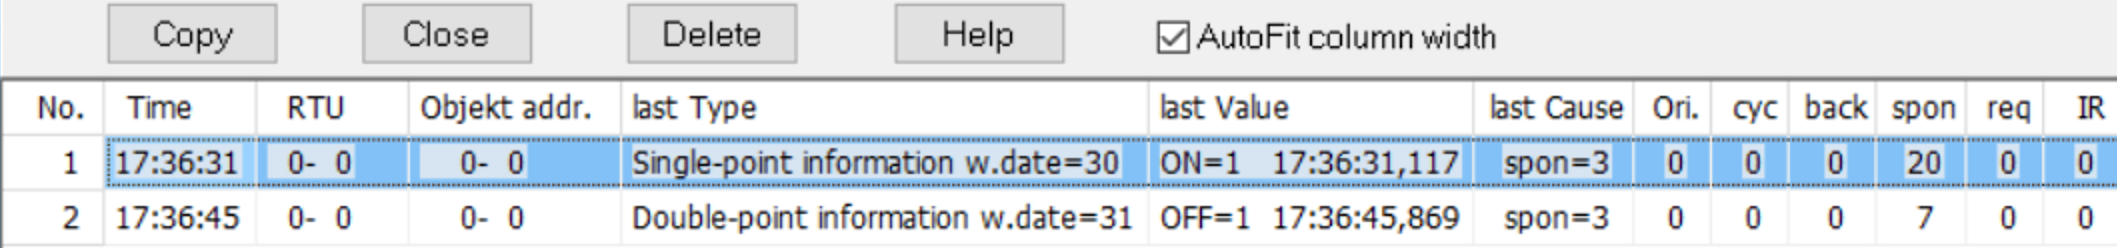
\includegraphics{WinPP104-PI}}
    \caption{Obraz procesov programu WinPP104}
\label{ProcessImage}
\end{figure} \par
\noindent \textbf{Zhrnutie:} WinPP104 je veľmi dobre vytvorený emulačný a monitorovací nástroj. Veľkou výhodou je, že dokáže jednotlivé zariadenia aj emulovať. 
Navyše pri monitorovaní alebo emulovaní zariadenia program automaticky vytvára tzv. obraz procesov (process image) o jednotlivých zariadeniach a komunikácii s nimi. Obraz procesov je dobrý na rýchly prehľad stavu jednotlivých objektov. Tiež je možné vyfiltrovať iba určitú komunikáciu podľa nami zadaného filtra. Ukážka je na obrázku \ref{ProcessImage}. Obraz procesov je možné zobraziť cez {\tt View} $\rightarrow$ {\tt Process image}. \par
\noindent Počas behu programu vytvára systém tabuľku jednotlivých komunikácií, nazývanú tiež tabuľka TCP 104, viď obrázok \ref{WinPP104-TCP}. TCP 104 tabuľka je vhodná na rýchly prehľad aktívnych spojení, na filtrovanie spojení a sledovanie napr. nezabezpečených spojení (cez WiFi) alebo zariadení, ktoré sa nechovajú podľa očakávaní. \par
\begin{figure}[h]
    \centering
    \scalebox{0.4}{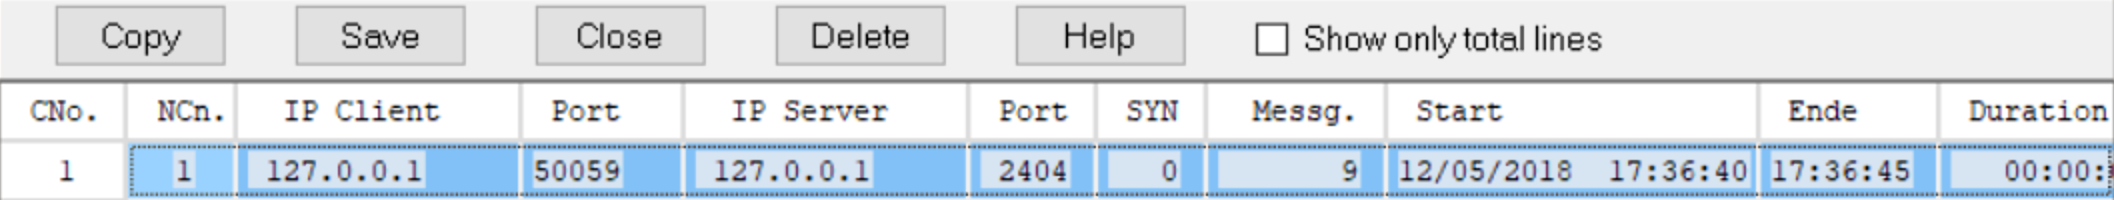
\includegraphics{WinPP104-TCP}}
    \caption{Prehľad TCP spojení programu WinPP104}
\label{WinPP104-TCP}
\end{figure}
\noindent Nevýhodou však zostáva, že program je voľne dostupný iba v rámci demoverzie, ktorá neumožňuje uloženie konfigurácií systému a je možné zaslanie a prijatie iba 20 správ medzi uzlami. Toto obmedzenie značne komplikuje konfiguráciu a dlhodobé sledovanie rozsiahlejších systémov. Taktiež je práca s programom relatívne komplikovaná a prvotné zorientovanie sa v systéme je o to náročnejšie. Pre porovnanie, nie je také intuitívne ako napr. v programoch Client/Server Simulator, ktoré budú popísané v predposlednej podkapitole.

\subsection{Knižnica OpenMUC - j60870}
\textbf{Výrobca:} OpenMUC je framework založený na jazyku Java a OSGi (špecifický interface pre jazyk Java), ktorý umožňuje jednoduchší vývoj špecifických monitorovacích, zaznamenávacích a riadiacich systémov. Framework bol vytvorený na Fraunhoferovom inštitúte pre solárne energetické systémy vo Freiburgu. Podporuje vývoj softwaru pre niekoľko komunikačných protokolov, napr.: \par
\begin{itemize}
\item M-Bus
\item IEC 61850 
\item IEC 62056-21
\item IEC 60870-5-104
\end{itemize} \par
\noindent \textbf{Popis produktu:} OpenMUC - j60870 je knižnica pre jazyk Java JDK\footnote{OpenMUC - j60870 \url{https://www.openmuc.org/openmuc/} [Online: Október 2017]}. Umožňuje vytvorenie (naprogramovanie) koncových staníc typu klient/server. Výsledný program môže slúžiť ako emulačný prostriedok ale aj ako reálne monitorovacie zariadenie. Vytvorené simulačné programy monitorovacích/meracích zariadení by podľa špecifikácie výrobcu mali byť schopné komunikovať s akýmkoľvek zariadením využívajúcim protokol IEC 60870-5-104. \par
\noindent \textbf{Protokoly:} Knižnica implementuje komunikačný štandard IEC 60870-5-104. \par
\noindent \textbf{Zariadenia:} Po naprogramovaní vlastného programu klient/server je možné pripojiť alebo sa pripojiť k reálnemu fyzickému IEC monitorovaciemu/meraciemu zariadeniu, prípadne k zariadeniam emulovaným iným programom. \par
\noindent \textbf{Typ:} Knižnica j60870 je licencovaná pod GPLv3. Je možné si od výrobcu zakúpiť proprietárnu licenciu. \par
\noindent \textbf{Platforma:} S knižnicou je možné pracovať pod OS Windows alebo pod akýmkoľvek UNIX-like OS. Ja osobne som s knižnicou pracoval pod Mac OSX. Bohužiaľ nie je k dispozící nijaké GUI, ani vývojové prostredie na vytvorenie vlastných zariadení, kedže ide iba o knižnicu rozširujúcu možnosti jazyka Java. \par
\noindent \textbf{Prípadová štúdia:} V rámci knižnice sú už predpripravené dva ukážkové programy, jeden pre klienta, druhý pre server. Programy sú uložené v zložke {\tt j60870/run-scripts}. Pomocou programov je ale možné vytvoriť iba jednoduché spojenie obsahujúce jedného klienta a server obsahujúci jedno koncové zariadenie. Počas testovania bola použitá rovnaká topológia ako pri programe WinPP104. Viď obrázok \ref{WinPP104-Topology}. Pre zložitejšie topológie je potrebné si naprogramovať vlastné stanice klient/server. Pri programovaní je možné využiť množstvo funkcí, ktoré knižnica poskytuje práve na takúto implementáciu. Documentáciu jednotlivých funkcií, ktoré knižnica obsahuje je možné nájsť na \footnote{JavaDoc \url{https://www.openmuc.org/iec-60870-5-104/javadoc/} [Online: Október 2017]}. V rámci testovania boli spustené oba predpripravené programy na jednom zariadení. Boli spustené v termináli (každý v samostatnom okne) daného zariadenia príkazom {\tt ./j60870-sample-server/j60870-console-client}. Program servera neumožňoval žiadnu interakciu od užívateľa, iba prijímal príkazy od klienta. V rámci programu klienta bolo možné posielať príkazy na synchronizáciu času a na čítanie hodnoty zo servera, posielať príkazy na zmenu hodnôt na servery nebolo možné. Testovanie slúžilo k preukázaniu, že programy naprogramované v knižnici j60870 sú schopné bežnej komunikacie pomocou protokolu IEC 60870-5-104. Na základe zachytenej komunikácie sa to preukázalo. Komunikácia bola zachytená pomocou nástroja Wireshark na rozhraní loopback. Bol vytvorený súbor j60870.pcap uložený v github repozitári \footnote{GitHub \url{https://github.com/janpristas/bakalarska-praca}}. \par
\noindent \textbf{Zhrnutie:} Výhodu v knižnici j60870 vidím v tom, že si užívateľ môže vytvoriť monitorovacie alebo meracie zariadenia presne na mieru, nakoľko si ich vytvorí priamo v zdrojovom kóde. Nevýhodou ale je, že práca s touto knižnicou už vyžaduje pokročilejšie znalosti a zručnosti s jazykom Java a s programovaním ako takým.

\subsection{IEC 60870-5-104 Client/Server Simulator}
\textbf{Výrobca:} FreyrSCADA \& Embedded Solution je indická spoločnosť so zameraním na vývoj softwaru pre rôzne komunikačné protokoly\footnote{FreyrSCADA \& Embedded Solution \url{http://freyrscada.com} [Online: November 2017]}. Mimo iné medzi ne patria:
\begin{itemize}
\item IEC 60870-5-101
\item IEC 60870-5-103
\item IEC 60870-5-104
\item DLMS/COSEM Client
\end{itemize}
\noindent \textbf{Popis produktu:} Vyššie uvedená spoločnosť ponúka hneď dva produkty pre protokol IEC-60870-5-104. Jeden na emuláciu klient (master) staníc a druhý na emuláciu server (slave) staníc. Každý program umožňuje emulovať až 50 uzlov klient/server a každý uzol navyše niekoľko koncových staníc. Jednotlivé nástroje umožňujú prenos dát a príkazov spolu s uložením .log správy s prehľadom aktuálnej komunikácie, ktorá na nich prebieha. Zdrojové kódy sú písané v jazyku C. \par
\noindent \textbf{Protokoly:} Oba programy sú určené na prácu výhradne nad protokolom IEC 60870-5-104. \par
\noindent \textbf{Zariadenia:} Programy si emulujú svoje vlastné koncové zariadenia, dokážu sa ale pripojiť aj k zariadeniam emulovaným iným programom, prípadne k reálnym fyzickým zariadeniam. \par
\noindent \textbf{Typ:} Program nie je open source, ale výrobca poskytuje zdarma demo verziu oboch programov. Demo verzia má však nevýhodu v tom, že po spustení má užívateľ iba 15 minút na prácu. Po uplynutí tohto času je nutné program vypnúť a spustiť znovu, spolu s opätovnou konfiguráciou klient/server staníc. Je to veľká nevýhoda, ak chcete testovať väčšiu sieť, kde iba samotné vytvorenie zaberie veľa času a na testovanie už nijaký nezostane. \par
\noindent \textbf{Platforma:} Samotné programy sú určené iba na OS Windows. Výrobca ale poskytuje aj tzv. SDK (Software Development Kit), pre klienta aj server, ktore obsahujú programy v jazyku C a umožňujú naprogramovanie koncových staníc s presnými špecifikáciami požadovanými zákazníkom. Programy SDK sú dostupné na OS Windows aj Linux. \par
\noindent \textbf{Prípadová štúdia:} Program klienta môže mať v rámci jedného uzlu pripojený iba jeden server, pričom server môže obsahovať niekoľko koncových zariadení. Je možné ale vytvoriť až 50 rôznych spojení klient/server. Pri vytváraní nového klienta/servera ponúka emulátor defaultné nastavenia, ktoré je možne vidieť na obrázku \ref{ClientConf} a \ref{ServerConf}. Prvotná konfigurácia je o niečo náročnejšia, nakoľko má program viac možností konfigurácie ako vyššie popisované programy. K dispozícií je ale niekoľko inštruktážnych videí\footnote{Tutoriály \url{http://freyrscada.com/iec-60870-5-104-Client-Simulator.php} [Online: November 2017]}, ktoré podrobne popisujú prácu s jednotlivými programami. Oba programy sú veľmi dobre spracované a umožňujú užívateľovi podrobnú konfiguráciu jednotlivých staníc podľa jeho potreby. V rámci klienta je možné nastaviť parametre ako ip adresu, port, počet pripojených staníc, adresy jednotlivých staníc a pod. V rámci servera takisto ip adresu, port, ip adresu klienta, dĺžku trvania jednotlivých typov príkazov a pod. Podrobnejšie je to možné vidieť na obrázku \ref{ClientConf} a \ref{ServerConf}.
\begin{figure}[h]
    \centering
    \begin{minipage}[b]{0.4\textwidth}
    \centering
    \scalebox{0.5}{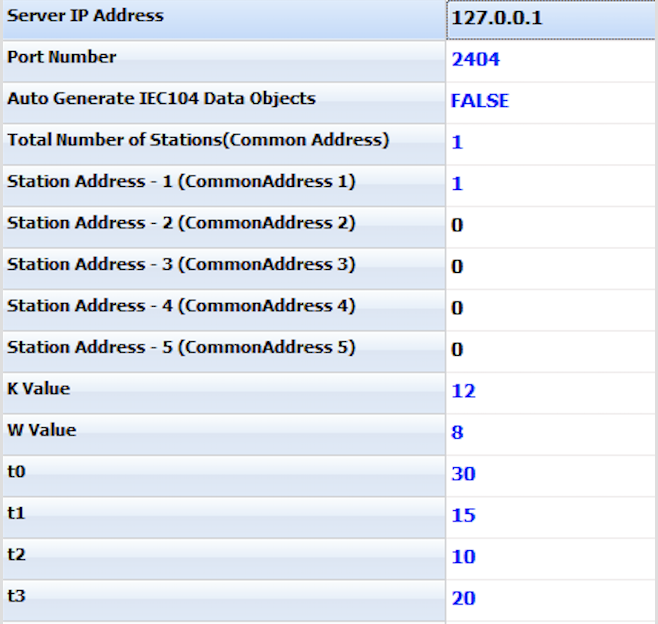
\includegraphics{IEC-Configuration}}
    \caption{Defaultná konfigurácia nového klienta}
    \label{ClientConf}
    \end{minipage}
    \begin{minipage}[b]{0.4\textwidth}
    \centering
    \scalebox{0.52}{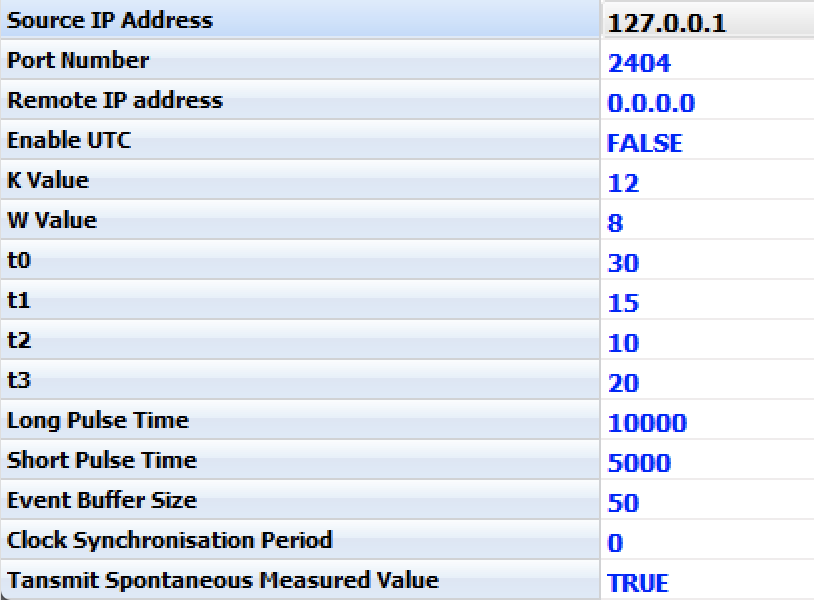
\includegraphics{IECS-Configuration}}
    \caption{Defaultná konfigurácia nového servera}
    \label{ServerConf}
    \end{minipage}
\end{figure} \par
Vytvorenie spojenia a testovanie programov pozostávalo z niekoľkých krokov:
\begin{enumerate}
\item Spustenie programu servera
\item Kliknutie na {\tt Add Server}
\item Komunikácia prebiehala na rozhraní loopback, nebolo treba nič nastavovať čo sa týka spojenia
\item {\tt Configuration} $\rightarrow$ {\tt Add Row}:
\begin{itemize}
\item {\tt Group} $\rightarrow$ {\tt Measured Short Float}
\item {\tt Type Id} $\rightarrow$ {\tt M\_ME\_NC\_1 = 13}
\item {\tt Starting IOA} $\rightarrow$ 1
\item {\tt Range} $\rightarrow$ 5
\end{itemize}
\item {\tt Add Row}
\begin{itemize}
\item {\tt Group} $\rightarrow$ {\tt Set Point Command - Float Value}
\item {\tt Type Id} $\rightarrow$ {\tt C\_SE\_NC\_1 = 50}
\item {\tt Starting IOA} $\rightarrow$ 10
\item {\tt Range} $\rightarrow$ 5
\end{itemize}
\item {\tt Load Configuration}
\item {\tt Data\_Objects}
\item Následne bolo potrebné všetky objekty typu {\tt Set Point} (začínajúce číslom 10) namapovať na objekty uchovávajúce namerané hodnoty:
\begin{enumerate}
\item Pravý klik na objekt
\item {\tt Map}
\item V zozname vybrať objekt na ktorý sa ide mapovať, ideálne 10 $\rightarrow$ 1, atp.
\end{enumerate}
\item {\tt Start Communication}
\item Spustenie programu klienta
\item {\tt Add Client}
\item Nebolo potrebné nastavovať IP adresu, ani port, komunikácia prebiehala na rozhraní loopback na štandardnom porte 2404
\item {\tt Data\_Objects} $\rightarrow$ {\tt Start Communication}
\item Klient sa pripojil k serveru a zobrazil pripojené objekty
\end{enumerate}
Po kliknutí pravým tlačítkom na jednotlivé objekty sa zobrazili príkazy, ktoré bolo možné zasielať serveru. {\tt Point Command} na vzdialené nastavenie hodnôt, {\tt Station Commands} na zaslanie štandardných príkazov typu {\tt General Interrogation}, {\tt Counter Interrogation}, {\tt Directory Read} atp. Priebeh komunikácie je možné vidieť v logovacej správe, ktorá je automaticky generovaná oboma programami. Správu je možné zobraziť po rozkliknutí záložky {\tt Log}. \par
Testovanie spočívalo v zaslaní niekoľkých štandardných príkazov medzi klientom a serverom na overenie, že komunikácia odpovedá štandardom protokolu IEC 60870-5-104. Zaslané príkazy boli zamerané hlavne na vzdialené čítanie a nastavenie hodnôt. Na obrázku \ref{iectopology} je ukázaná topológia použitá pri testovaní. 
\begin{figure}[h]
    \centering
    \scalebox{0.8}{\includegraphics{iec_topology}}
    \caption{Ukážka testovacej topológie programov Client/Server Simulator}
\label{iectopology}
\end{figure}
Programy boli spustené na jednom zariadení. Komunikácia bola zachytávaná pomocou nástroja RawCap na rozhraní loopback. Zachytená komunikácia je v súbore C/SSimulator.pcap, ktorý je uložený v github repozitári \footnote{GitHub \url{https://github.com/janpristas/bakalarska-praca}}. \par
\noindent \textbf{Zhrnutie:} Client/Server Simulator programy sú asi najprehladnejšie varianty s najväčšou škálou možností na emuláciu prevádzky SCADA systémov využívajúcich protokol IEC 60870-5-104. Veľkou nevýhodou ale zostáva, že demoverzie, s ktorými som pracoval, poskytujú iba 15 minút na prácu a následne sa vypnú. Celý systém je potom nutné konfigurovať odznova.

\subsection{QTester 104}
\textbf{Výrobca:} Autorom produktu je Ricardo Olsen, majiteľ spoločnosti DSC Systems. Jeho prácou je konfigurácia a vývoj riadiacich systémov pre komunikáciu klient/server. \par
\noindent \textbf{Popis produktu:} QTester 104 je open source software, ktorý slúži na získavanie dát z koncových staníc a ich riadenie. Je možné si ho zdarma stiahnuť na stránke {\tt sourceforge.net}\footnote{QTester 104 \url{https://sourceforge.net/projects/qtester104/} [Online: Október 2017]}. Umožňuje sledovať stav koncových zariadení, sťahovať z nich dáta a posielať príkazy. Pracuje iba ako klient(master). Je vytvorený v C++ za pomoci QT. Záznam komunikácie je možné uložiť vo forme textového dokumentu. Software je iba časťou väčšieho HMI projektu\footnote{OSHMI \url{https://sourceforge.net/projects/oshmiopensubstationhmi/} [Online: November 2017]} a slúži ako modul pre HMI. Môže byť ale použitý aj samostatne ako protokol tester. \par
\noindent \textbf{Protokoly:} Program využíva na komunikáciu protokol IEC 60870-5-104. \par
\noindent \textbf{Zariadenia:} Kedže QTester 104 funguje iba ako klient, nie je schopný emulovať koncové zariadenia. Je možné ale pripojiť reálne, alebo iným programom emulované zariadenia. Komunikácia prebieha cez TCP/IP spojenie. \par
\noindent \textbf{Typ:} Program je open source a je spolu so zdrojovými kódmi voľne k dispozíci. Taktiež ho je možné voľne distribuovať ďalej. \par
\noindent \textbf{Platforma:} S programom je možné pracovať pod OS Windows a Linux. Na obrázku \ref{QTester} je ukážka užívateľského rozhrania programu. \par
\begin{figure}[h]
	\centering
    \scalebox{0.35}{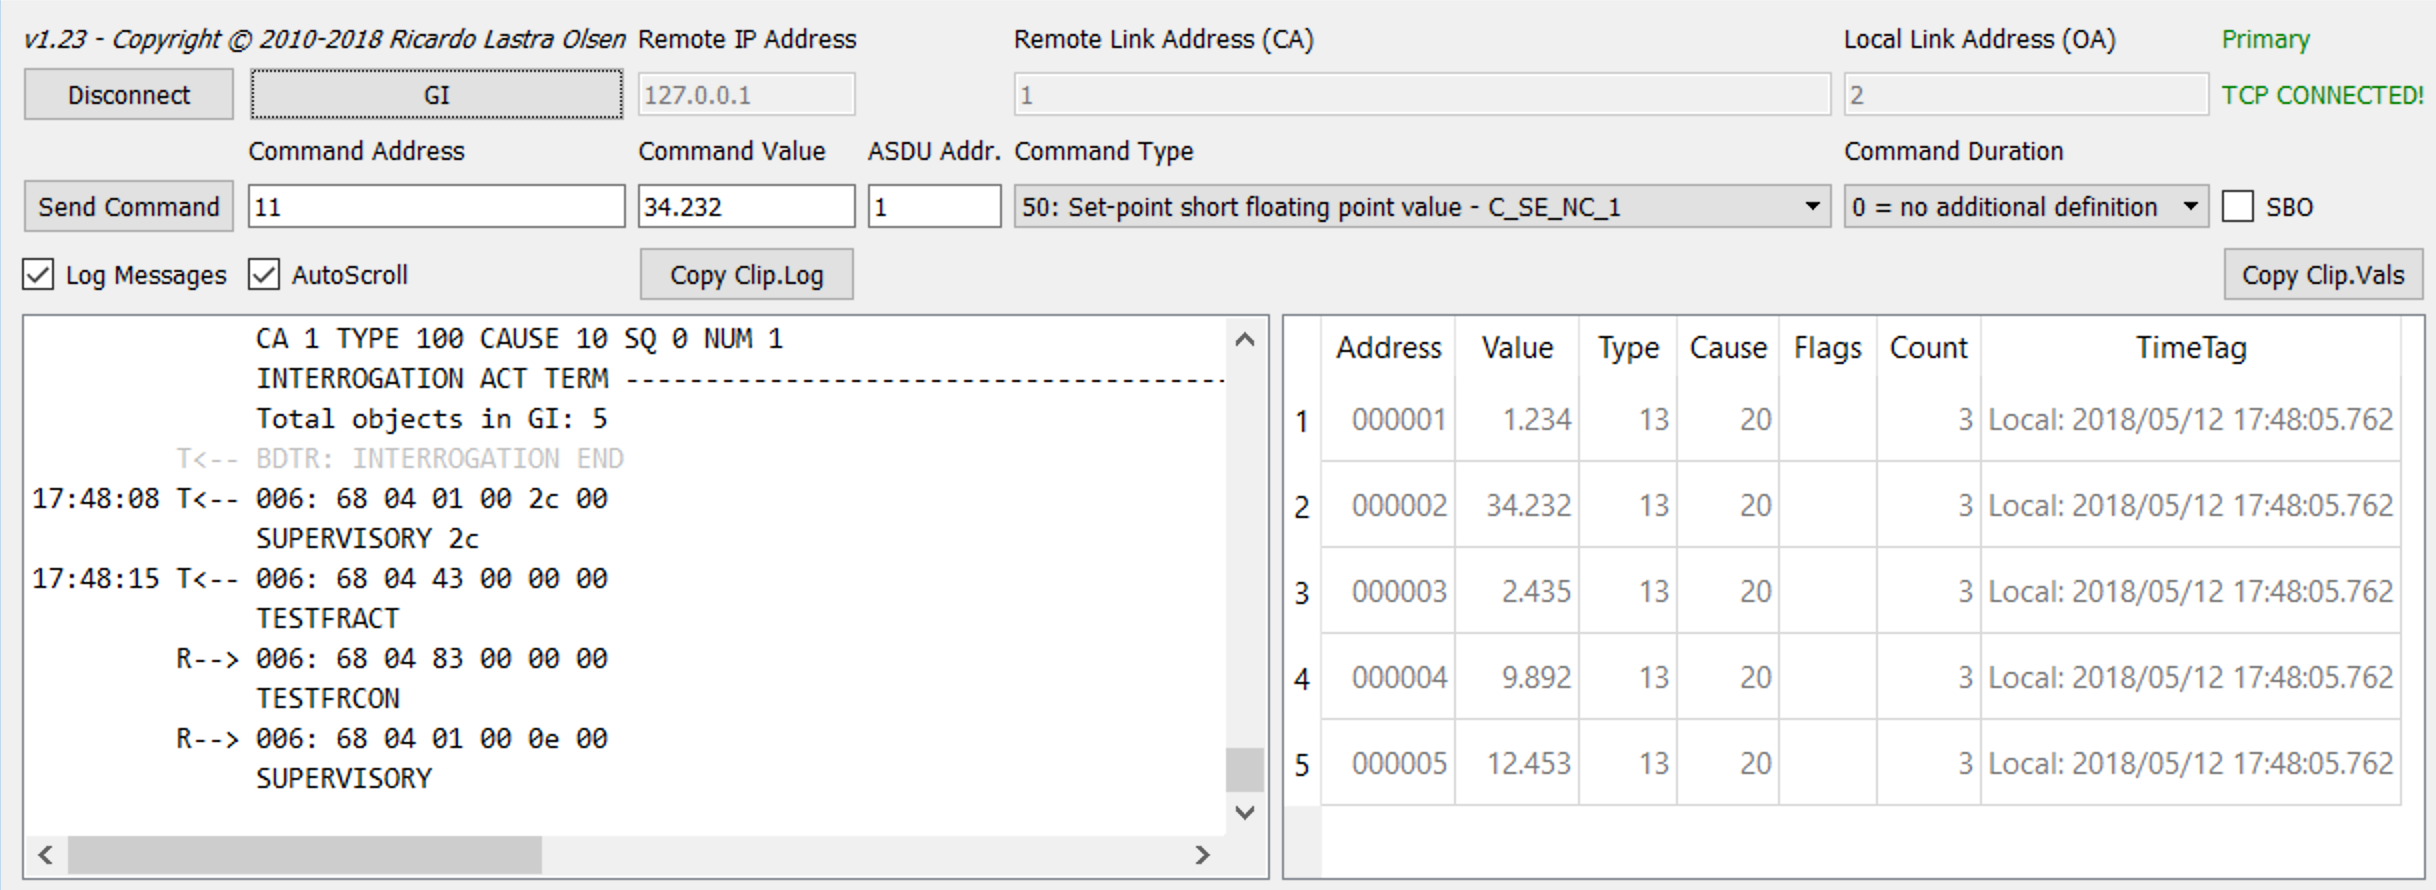
\includegraphics{QTester}}
    \caption{Ukážka užívateľského rozhrania programu QTester 104}
\label{QTester}
\end{figure}
\noindent \textbf{Prípadová štúdia:} QTester 104 umožňuje v rámci monitorovania mať vytvorenú iba jednú stanicu pre klienta, čo je vlastne program samotný, a umožňuje pripojenie jednej stanice servera. Testovanie prebiehalo pod OS Windows za pomoci programu IEC 104 Server Simulator, ktorý bol popísaný v predchádzajúcej podkapitole. \par
Vytvorenie testovacej topológie prebiehalo v niekoľkých krokoch:
\begin{enumerate}
\item Spustenie a konfigurácia servera, rovnako ako v predchádzajúcej podkapitole
\item Spustenie programu QTester 104: {\tt qtester104} $\rightarrow$ {\tt bin} $\rightarrow$ {\tt QTester104}
\item Pri testovaní bolo použité rozhranie loopback na ktorom sa program ihneď po spustení snažil spojiť so serverom, nebola potrebná dodatočná konfigurácia
\item Po úspešnom spojení, kliknúť na {\tt GI (General Interrogation)} aby sa načítali objekty pripojené k serveru
\item Zakliknúť {\tt Log Messages}, prípadne {\tt AutoScroll} na zobrazenie logovacej správy
\end{enumerate}
Po úspešnej konfigurácií a prepojení je možné zasielať serveru príkazy. Pre zaslanie príkazu je potrebné nastaviť niekoľko hodnôť:
\begin{itemize}
\item {\tt Command Address}, adresa {\tt Set-point} objektu namapovaného na objekt, ktorý chceme nastaviť, napr. 10
\item {\tt Command Value}, hodnota na ktorú chceme objekt nastaviť, musí byť typu čísla s pohyblivou rádovou čiarkou, napr 123.456
\item {\tt ASDU address}, hodnotu nastaviť na 1
\end{itemize} \par
Práca s programom je vo všeobecnosti veľmi intuitívna, po spustení stačí iba zadať IP adresu servera, program sa s ním automaticky spojí a je možné s ním ihneď pracovať. Na obrázku \ref{QTester104} je ukážka stavu programu ihneď po spustení.
\begin{figure}[h]
    \centering
    \scalebox{0.43}{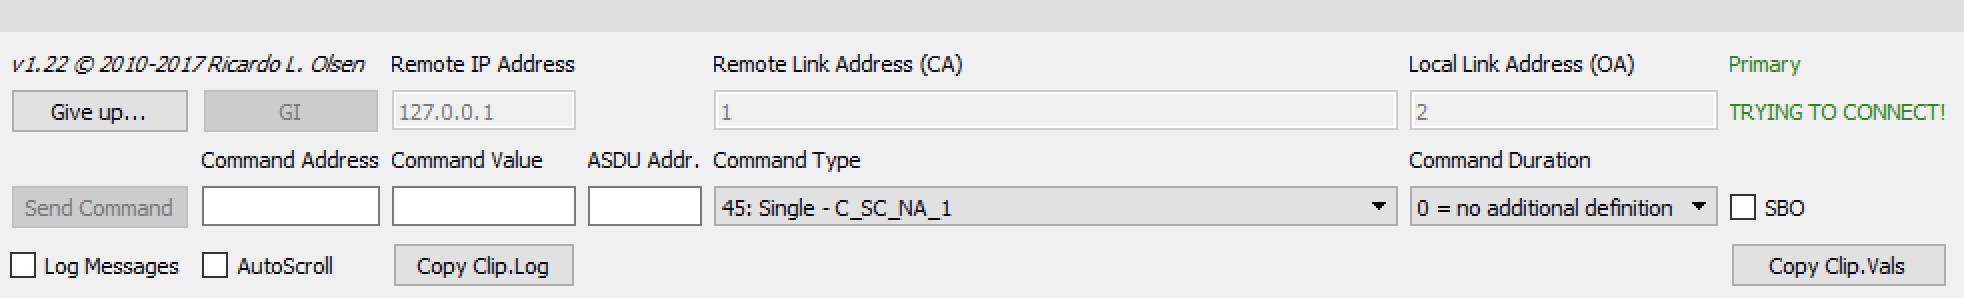
\includegraphics{QTester104}}
    \caption{Defaultné nastavenie programu pri spustení}
\label{QTester104}
\end{figure}
Pri každej zmene hodnôt na strane servera sú automaticky aktualizované v QTestery. Pri testovaní bolo vytvorených päť koncových zariadení typu {\tt M\_ME\_TF} na zaznamenávanie hodnôt s pohyblivou rádovou čiarkou. Topológiu je možné vidieť na obrázku \ref{QT-Topology}.
\begin{figure}[h]
    \centering
    \scalebox{0.8}{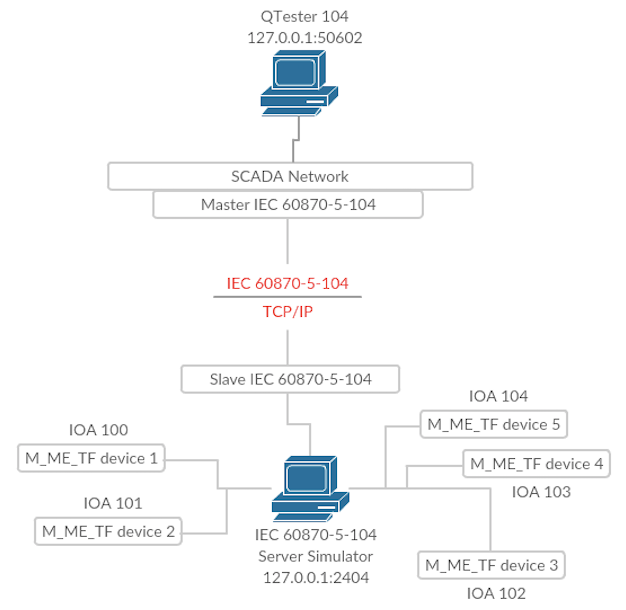
\includegraphics{QT-Topology}}
    \caption{QTester 104 - Testovacia topológia}
\label{QT-Topology}
\end{figure}
Oba programy boli spustené na jednom zariadení a komunikácia medzi nimi bola následne odchytávaná v nástroji RawCap na rozhraní loopback. Z komunikácie bol vygenerovaný súbor QTester104.pcap uložený v github repozitári \footnote{GitHub \url{https://github.com/janpristas/bakalarska-praca}}. \par
\noindent \textbf{Zhrnutie:} QTester 104 je celkom prepracovaný a užívateľsky prívetivý monitorovací nástroj. Výhodou je, že je open source a je možné s ním voľne pracovať a distribuovať ho. Ďalšiu výhodu vidím v jednoduchom a intuitívnom GUI v ktorom sa veľmi dobre pracuje. Nevýhodou je menšia škála možností oproti programu Client Simulator z predchádzajúcej kapitoly, na testovacie účely bol ale postačujúci.

\section{Zhrnutie}
\tab V tejto kapitole bol uvedený základný prehľad priemyselných monitorovacích a emulačných nástrojov pre SCADA systémy. Bola popísaná najmä ich základná funkcionalita a schopnosť komunikácie odpovedajúcej patričným štandardom. \par
\subsection{DLMS/COSEM}
\par
\begin{tcolorbox}[enhanced, title={Porovnanie emulátorov pre protokol DLMS/COSEM}, clip upper, fontupper=\sffamily,%
    tabularx={>{\cellcolor[gray]{.5}\color{white}}r%
              >{\centering\arraybackslash}X%
              >{\centering\arraybackslash}X}]
  &\cellcolor{black!80}\color{white} DLMS Director   &\cellcolor{black!80}\color{white} XmlDemo \\
Platforma       & OS Windows                         & OS Windows \\
Klient/Server   & Klient                             & Klient \\
Kom. protokoly  & TCP/IP, HDLC                       & TCP/IP, HDLC iba cez sériovú linku \\
Licencia        & Open Source                        & Open Source \\
Vlastná konfig. & Nie, iba objekty pripojené k serveru & Nie, iba objekty pripojené k serveru \\
GUI             & Veľmi dobré a intuitívne           & Veľmi jednoduché \\
Celkový dojem   & Dobre spracovaný program s veľkou škálou možností  & Dobre spracovaný program podporujúci základnú potrebnú funkčnosť
\end{tcolorbox} \par 
Pre protokol DLMS/COSEM boli popísané programy DLMS Director a XmlDemo. Oba programy sú dobre spracované a poskytujú potrebnú funkčnosť a umožňujú vytvoriť komunikáciu odpovedajúcu štandardu DLMS/COSEM, avšak program DLMS Director poskytuje navrch možnosť komunikácie pomocou HDLC, väčšiu škálu možných nastavení a taktiež má oveľa prívetivejšie a intuitívnejšie GUI. Pre protokol DLMS/COSEM budem ďalej využívať program DLMS Director.

\subsection{IEC 60870-5-104}
\par
\begin{tcolorbox}[enhanced, title={Porovnanie emulátorov pre protokol IEC 104, 1. časť}, clip upper, fontupper=\sffamily,%
    tabularx={>{\cellcolor[gray]{.5}\color{white}}r%
              >{\centering\arraybackslash}X%
              >{\centering\arraybackslash}X}]
  &\cellcolor{black!80}\color{white} WinPP104   &\cellcolor{black!80}\color{white} Knižnica OpenMUC - j60870 \\
Platforma               & OS Windows            & OS Windows/Unix like OS \\
Klient/Server           & Klient/Server         & Klient/Server \\
Kom. protokoly          & TCP/IP                & TCP/IP \\
Licencia                & Demoverzia           & Licencovaná pod GPLv3 \\
Vlastná konfig.         & Možnosť konfigurácie vlastných šablón správ & Možnosť vytvoriť si vlastný program klient/server podľa potreby užívateľa \\
GUI                     & Trochu komplikované   & Vzorové programy bez GUI, iba ako terminálové aplikácie \\
Celkový dojem           & Program je relatívne náročný na prvotné zorientovanie a pochopenie, taktiež je nevýhodou obmedzenie demoverzie na zaslanie/prijatie iba 20 správ & Vzorové programy jednoduché (slúžia iba na ilustráciu možností knižnice), knižnica je dobre spracovaná, umožňuje veľkú škálu možností na tvorbu vlastných staníc
\end{tcolorbox}

\begin{tcolorbox}[enhanced, title={Porovnanie emulátorov pre protokol IEC 104, 2. časť}, clip upper, fontupper=\sffamily,%
    tabularx={>{\cellcolor[gray]{.5}\color{white}}r%
              >{\centering\arraybackslash}X%
              >{\centering\arraybackslash}X}]
  &\cellcolor{black!80}\color{white} Client/Server Simulator &\cellcolor{black!80}\color{white} QTester 104 \\
Platforma   & OS Windows, možnosť získať SDK pre klienta a server od výrobcu na OS Windows/Linux & OS Windows/Linux \\
Klient/Server   & Klient/Server & Klient \\
Kom. protokoly    & TCP/IP & TCP/IP \\
Licencia & Demoverzia & Open Source \\
Vlastná konfig. & Nie, možnosť využívať iba štandardné objekty & Nie, iba objekty pripojené k serveru \\
GUI    & Dobre spracované, miestami trochu komplikované & Veľmi dobré, jednoduché a intuitívne \\
Celkový dojem   & Veľmi dobre spracované programy s veľkou škálou možností, nevýhodou je obmedzenie na 15 minút pri demoverzií & Veľmi dobre spracovaný program, veľmi jednoduchý, podporujúci základnú požadovanú funkcionalitu
\end{tcolorbox} \par
Pre protokol IEC 60870-5-104 boli popísané programy WinPP104, QTester 104, IEC 60870-5-104 Client/Server Simulator a knižnica pre jazyk Java OpenMUC - j60870. Každý z programov poskytuje inú funkcionalitu a škálu možností konfigurácie. Všetky programy umožňujú vytvoriť komunikáciu odpovedajúcu štandardu IEC 60870-5-104. Užívateľsky najprívetivejšie a pre ďalšie testovanie sú najvhodnejšie programy Client/Server Simulátor a QTester 104. Programy podporujú veľkú škálu možností na konfiguráciu staníc a špecifikáciu komunikácie. Taktiež poskytujú veľmi intuitívne prostredie a pracuje sa s nimi jednoducho. Oproti tomu je program WinPP104 oveľa komplikovanješí a práca s ním nie je jednoduchá. \par 
Rovnako komplikovaná je práca s knižnicou OpenMuc - j60870, ktorá síce umožňuje vytvorenie vlastného programu klient/server, vyžaduje však vyššiu znalosť programovacieho jazyka Java a problematiky samotnej. Výhodou programu QTester 104 je jeho voľná dostupnosť a kvalitné spracovanie. Nevýhodou ale zostáva možnosť vytvorenia spojenia iba medzi jedným klientom a serverom. Tento problém riešia programy IEC 60870-5-104 Client/Server Simulator, ktoré umožňujú vytvorenie väčšej~topológie. Avšak nevýhodou demoverzie je časové obmedzenie, ktoré umožňuje s programami pracovať maximálne 15 minút. \par
V praktickej časti svojej práce budem vychádzať z programov DLMS Director, QTester 104 a IEC 60870-5-104 Client/Server Simulator.
  \chapter{Bezpečnosť SCADA systémov}
\label{bezpecnost}
\tab Počítačové útoky sú v dnešnej dobe skutočnou hrozbou. Jedným z hlavných dôvodov ohrozenia SCADA systémov je ich postupný prechod na IP vrstvu. Systémy sa stále rozrastajú a vzdialenosť jednotlivých koncových staníc od riadiacej je čoraz väčšia, čo znemožňuje systému komunikovať na fyzickej vrstve. Je preto potrebné vytvoriť komunikačný kanál (napr. VPN spojenie), na vzdialené monitorovanie, medzi jednotlivými stanicami. Na jednej strane je to užívateľsky veľmi prívetivé, je možné vzdialene sledovať a riadiť veľmi veľké množstvo zariadení. Taktiež je možné centrálne vykonávať rôzne aktualizácie ap. Avšak vytvorenie komunikačného kanálu v značnej miere zjednodušuje útočníkom napadnúť a infikovať danú sieť, nakoľko komunikačný kanál môže byť použitý ako zadný vchod (backdoor) do systému. Preto je potrebné komunikáciu v sieti neustále monitorovať (flow monitorovanie) a mať k dispozícií nástroje (rôzne sondy ap.), ktoré sú schopné zachytiť neštandardnú komunikáciu v sieti a včas varovať pred bezpečnostným incidentom. Dôsledky jednotlivých incidentov sa môžu pohybovať od relatívne malých, ako je napríklad prerušenie prebiehajúcej operácie alebo zmena operačného procesu po veľké, ako úmyselné sabotáže s cieľom spôsobiť systému citeľnú ujmu. Jednotlivé útoky nemusia mať vplyv iba na systém samotný, ale aj na okolitú spoločnosť. Napríklad útoky na veľké komplexy ako elektrárne, rafinérie, čističky môžu mať veľký dopad aj na životné prostredie (únik ropy, uvoľnenie toxických látok). Niektoré útoky môžu mať dokonca za následok zranenia alebo straty na životoch, potencionálne katastrofické výbuchy ap\cite{Security}. \par
Úspešný útok môže mať mnoho rôznych následkov zahŕňajúc:
\begin{itemize}
\item zmeny alebo blokovanie zamýšlaného procesu, napr. zmeny v zamýšlanom množstve vyrobenej el. energie,
\item zmeny, oneskorenie alebo blokovanie v infomácií o nameraných hodnotách, veľký dôsledok môže mať napríklad pri obchodovaní s energiami,
\item neautorizované zmeny v inštrukciách, prípadné vypnutie jednotlivých zariadení ako generátory.
\end{itemize}
Konečným dôsledkom útoku môže byť čokoľvek od finančnej straty až po stratu fyzického zabezpečenia systému s dopadom na okolný ekosystém, miestnu komunitu, prípadne dokonca aj štát. Stručný prehľad dopadu útokov rôznych veľkostí je na obrázku \ref{attackcons}.
\begin{figure}[h]
    \centering
    \scalebox{0.55}{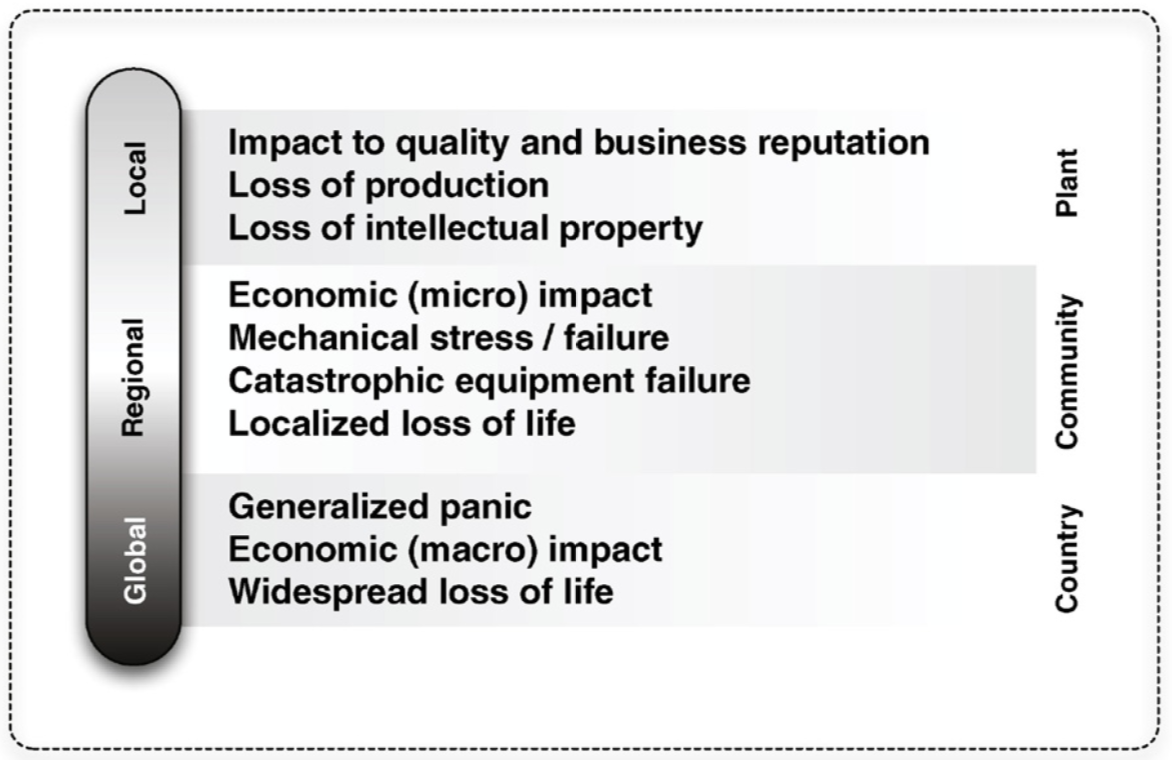
\includegraphics{security_impact}}
    \caption{Dopad rôznych druhov útokov\cite{Security}}
\label{attackcons}
\end{figure}

\section{Bezpečnostné riziká}
\tab Pri posudzovaní bezpečnosti a bezpečnostných rizík v SCADA systémoch sa rozlišuje medzi dvoma typmi útokov. Útoky cez SCADA kanále (SCADA channels) a útoky cez podporné kanále (maintenance channels)\cite{Security}. \par
SCADA kanále sú komponenty slúžiace na primárne účely SCADA systémov - zber a prenos dát, skladovanie a spracovanie údajov a informácií z komunikácie medzi jednotlivými komponentami systému. Medzi typické komponenty SCADA systémov patria:
\begin{itemize}
\item Systém riadenia distribúcie - súbor aplikácií na sledovanie a riadenie systému
\item SCADA servery
\item Vzdialené koncové zariadenia
\item Inteligentné meracie zariadenia
\item Ochranne články
\end{itemize}
Podporné kanále sú systémy slúžiace na inštaláciu a údržbu vyššie spomenutých súčastí systému. Taktiež slúžia na sprostredkovanie komunikácie medzi nimi. Typicky to sú:
\begin{itemize}
\item Inžinierske stanice
\item Spúšťacie (commissioning) servery
\item Servery na synchronizáciu času v systému
\item Monitorovacie a logovacie servery (SNMP, syslog)
\end{itemize} \par
Hlavným dôvodom rozlišovania medzi jednotlivými súčasťami systému je to, že každý so sebou nesie rozličné bezpečnostné riziká. Komunikácia cez SCADA kanály je väčšinou typu počítač-počítač a prenašajú sa iba prevádzkové data, nie konfiguračné zmeny alebo binárky. Narušenie alebo zneužitie sa v monitorovanej komunikácií dá ťažko skryť. To znamená, že je väčšina útokov relatívne rýchlo detekovateľná. Avšak pri podporných kanáloch je to o niečo komplikovanejšie. Autorizované zmeny na jednotlivých komponentoch vykonané pracovníkom spoločnosti sa moc nelíšia od neautorizovaných zmien vykonaných útočníkom. A pretože podporné služby vyžadujú privilegovaný prístup do systému, je to veľmi lákavé pre útočníkov, ktorí chcú získať permanentnú kontrolu nad systémom. Je ale možné spoľahlivo monitorovať aj túto časť siete, avšak iba ak sa všetky podporné procesy vykonávajú "disciplinovane". \par
V počítačových sieťach obecne existuje mnoho rôznych druhov útokov. Avšak pri SCADA systémoch sa väčšina z nich neberie do úvahy, nakoľko je pri nich predpoklad dostatočného zabezpečenia systému a dôkladná konfigurácia firewallov na prepúšťanie iba najdôležitejšej komunikácie. To znamená, že očividné "diery"\ do systému by mali byť uzavreté. Napriek tomu ale zostáva niekoľko typov útokov, ktorými sú SCADA systémy ohrozené\cite{Security}:
\begin{itemize}
\item Útok cez SCADA kanál
\item Útok cez podporu SCADA serverov
\item Útok cez podporu koncových zariadení
\item Útok "zvnútra"
\end{itemize}
Táto práca je zameraná najmä na útoky cez SCADA kanále a cez podporu koncových zariadení.

\subsection{Útoky cez SCADA kanále}
\tab Pri samotnom získavaní prístupu do riadiaceho systému SCADA siete existuje iba niekoľko možností ako ho infikovať. Nakoľko je na prístup do systému vyžadovaná autentizácia, útočníci sa môžu do systému dostať dvoma spôsobmi. Prvý je získanie prístupu cez platné autentizačné údaje niekoho iného. Rozhrania na výmenu údajov cez IT sieť by však mali byť obmedzené na export dát, takže dopad útoku na systém nie je taký veľký. Druhý spôsob je do systému rozšíriť malware cez servery prístupné z IT domén. Ak bude software využívať zraniteľnosti systému, umožní tak útočníkovi robiť veľké zmeny v jadre systému a môže výrazne ovplyvniť a ohroziť celý systém. Pravdepodobnosť úspechu takéhoto útoku výrazne závisí na zabezpečení a počte zraniteľných miest, ktoré systém má. \par
Ďalším vstupným bodom do SCADA systému je útok na koncové stanice. Nakoľko systém väčšinou využíva veľa koncových staníc, niektoré z nich dokonca na odľahlých miestach, ani dobrá fyzická ochrana nemôže plne zabrániť prieniku do zariadenia a následne do systému. Či už ide o fyzický alebo kybernetický útok, takéto útoky väčšinou nespravia v systéme veľké škody, nakoľko ide o napadnutie jedného zariadenia a na ovplyvnenie viacerých by bolo potrebné viesť útok cez riadiacu stanicu. Samozrejme to ale záleží aj od použitej topológie, ktorá je využívaná na prepojenie riadiacej stanice a koncových staníc. \par
Útočníci môžu využiť zariadenia na koncových staniciach na prístup do systému s platnými autentizačnými údajmi, avšak ak je systém dostatočne zabezpečený, môžu nanajvýš posielať nesprávne/podvrhnuté informácie o nameraných hodnotách. Aby boli schopný spraviť väčšie škody, museli by napr. rozšíriť po systéme software, ktorý bude schopný ovládať väčšie množstvo koncových staníc. \par
Ďalší typ útoku je pripojenie do systému cez spojenie s riadiacim strediskom. Sú dva typy hrozieb, ktoré môžu byť takýmto útokom napáchané. Prvý je pripojenie cez vlastnú riadiacu stanicu s jednotlivými koncovými zariadeniami s využitím platných autentizačných údajov. Útočník tak môže napr. posielať neautorizované príkazy jednotlivým staniciam. Druhý útok spočíva vo využití zraniteľnosti systému, čo môže byť zneužité napr. na rozšírenie rôznych typov malware do siete. \par
Keď už útočník prenikne do systému, je schopný využívať jeho plnú funkcionalitu a rôznymi spôsobmi ho tak poškodiť\cite{Security}.

\subsection{Útoky cez koncové zariadenia}
\tab Vybavenie koncových staníc ako RTU (Remote Terminal Units - mikroprocesorom riadené zariadenia) alebo IED (Intelligent Electronic Devices - inteligentné merače) môžu byť väčšinou spravované z jednej centrálnej stanice. Ak útočník dokáže získať prístup k týmto hostom, napr. cez platné autentizačné údaje, môže zmeniť konfiguráciu jednotlivých zariadení. Ak zariadenie nie je konfigurované lokálne, môže byť konfigurované cez nejaké externé zariadenie ako napr. laptop, USB kľúč, pamäťovú kartu ap. To je opäť riziko na rozšírenie malware po sieti. \par
Ďalšia cesta, ako je možné napadnúť systém, je využiť zraniteľnosti jednotlivých zariadení na stanici. Nakoľko väčšinou využívajú normálny IT software, poskytujú tým útočníkom jednoduchú cestu do SCADA systému. Koncové stanice môžu byť napadnuté zo sieťovej strany ale aj cez koncové zariadenia, ak do nich niekto vloží malware, ktorý sa môže ďalej šíriť do siete. \par
Riziko architektúry SCADA systému je aj v tom, že je možné si vytvoriť vstup do systému pripojením vlastného zariadenia. To sa týka najmä koncových staníc, ktoré sú menej chránené ako riadiaca stanica\cite{Security}.
\section{Typy útokov}
\tab Keď sa raz útočník dostane do systému a identifikuje svoj cieľ, existuje mnoho spôsobov, ako ho poškodiť. Medzi najbežnejšie útoky patria:
\begin{itemize}
\item Man-in-the-middle
\item Denial-of-Servise (DoS)
\item Replay útoky
\end{itemize}
Hlavným dôvodom je kombinácia rôznych protokolov a slabá úroveň autentizácie, napr. prenos nezašifrovaných kľúčov po sieti, ktoré sa dajú jednoducho odchytiť a použiť na získanie neoprávneného prístupu do systému. V systémoch, ktoré tvoria spojitosť medzi niekoľkými systémami, ako napr. SCADA server, môže byť trvalá prítomnosť útočníka v riadiacej časti použitá ako základ sekundárneho útoku proti iným častiam siete. Pri takomto útoku je veľmi dôležitý rozdiel medzi ovládnutím cieľa a útokom samotným. Ovládnutie cieľa znamená prístup alebo schopnosť vykonávať s objektom neznámu činnosť. Napríklad spustenie určitého procesu s parametrami nad prípustné medze a tým zariadenie fyzicky poškodiť, prípadne poškodiť viaceré zariadenia, ktoré sú na ovládanom závislé. Útok je na druhej strane schopnosť útočníka vykonávať s cieľovým objektom nežiadúce akcie. V tomto prípade môže zariadenie pracovať, tak ako má, avšak schopnosť napadnúť zariadenie a spôsobiť, že vykoná akciu, ktorú obsluhujúci personál nepožadoval, môže mať negatívne následky. Takéto útoky bývajú spojované s využívaním funkčnosti a zraniteľných miest zariadení. To znamená, že zaslanie riadiacemu zariadeniu príkaz na vypnutie nepredstavuje slabosť zariadenia ako takého, avšak nedostatok overovania a autentizácie umožňuje útočníkovi zaslať nežiadúci príkaz, a tým na istý čas ochromiť systém. Obdobné útoky sú tzv. replay útoky\cite{Security}. \par

\subsection{Man-in-the-middle útok}
\tab Vo svojej práci sa budem najviac zaoberať tzv. útokom man-in-the-middle, ktorý pozostáva z odchytenej a následne zmenej komunikácie medzi dvoma zariadeniami. \par
Pri útoku typu man-in-the-middle sa hovorí o útoku kedy útočník sleduje komunikáciu medzi zariadeniami, odchytáva zasielané správy, mení ich a opätovne zasiela pôvodnému adresátovi. Zariadeniam sa zdá, že medzi sebou komunikujú priamo, avšak v skutočnosti komunikujú cez tretie zariadenie, ktoré ich odpočúva a môže interagovať (zasahovať, meniť zasielané správy). Na obrázku \ref{mitm} je úkažka typickej komunikácie pri útoku man-in-the-middle, spolu so zmenou v zasielanom príkaze. \par
\begin{figure}[H]
    \centering
    \scalebox{0.35}{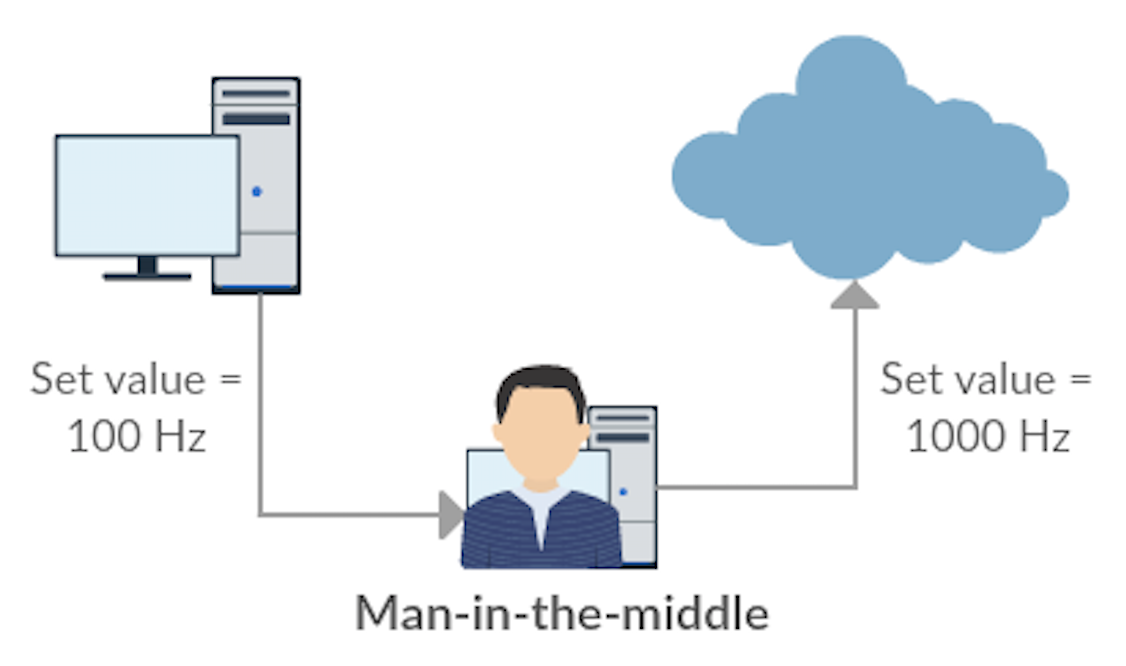
\includegraphics{mitm}}
    \caption{Man-in-the-middle útok}
\label{mitm}
\end{figure}
Ak chce útočník vykonávať man-in-the-middle útok, musí byť schopný zachytiť komunikáciu medzi oboma cieľovými systémami a vložiť do nej nové (upravené) správy. Ak spojenie nemá šifrovanie alebo dokonca ani overovanie autentizáciou, ako je častý prípad pri priemyselnej prevádzke, je man-in-the-middle útok veľmi jednoduchý proces. Avšak aj v komunikáciach, kde sa používa autentizácia, alebo šifrovanie, môže byť stále man-in-the-middle útok úspešný, napr. odpočúvaním kľúčových výmien a prenesením útočníkovho kľúča namiesto legitímneho. Tento spôsob útoku je ale v priemyselných sieťach trochu komplikovaný, nakoľko jednotlivé strany môžu spolu komunikovať dlhú dobu a útočník by musel zneužiť existujúce komunikačné spojenie. Najobtiažnejšou časťou úspešného man-in-the-middle útoku je úspešne prepojiť dátový tok a presvedčiť obe strany, že útočník je skutočne určeným príjemcom jednotlivých správ. Proti tomu je možné sa brániť autentizačnými kontrolami, avšak mnohé priemyselné komunikačné protokoly zasielajú autentizačné údaje v otvorenej podobe, čo uľahčuje útočníkovi prácu, nakoľko mu stačí odsledovať komunikáciu, prečítať autentizačný kľúč a úspešne sa pripojiť do systému\cite{Security}.

\subsection{Denial-of-Service útok}
\tab Denial-of-Service, čiže útok typu odoprenia služby, nastáva, keď sa nejaký útočník snaží odoprieť služby systému pre bežných užívateľov tým, že ho robí nedostupným (neschopným bežnej prevádzky). DoS útoky sú veľmi široká kategória útokov a môže zahŕňať čokoľvek od straty komunikácie so zariadením po narušenie alebo zablokovanie určitých služieb v rámci daného zariadenia (ukladanie, spracovanie I/O). DoS útoky v bežných systémoch väčšinou nemajú veľké následky, ak sú riešené včas. Avšak ak je DoS útok dobre cielený, môže prepnúť dôležité systémy do offline režimu, alebo ich dokonca vypnúť. \par
Automatizované systémy sa nasadzujú na monitorovanie a riadenie rôznych procesov. Tento proces môže ovplyvňovať tok ropy v potrubí, premenú vodnej pary na elektrinu alebo kontrolovať časovač zapaľovania v motore. Strata schopnosti správcu tieto procesy riadiť sa nazýva strata kontroly (Loss of Control - LOC) a zvyčajne vedie k prepnutiu fyzického procesu do "bezpečného"\ stavu vypnutia. To znamená, že aj jednoduché prerušenie kontrolných funkcií môže viesť k fyzickým poruchám na systéme, ktoré môžu pokračovať v odstavení systému, mechanickému zlyhaniu alebo iným katastrofickým scenárom. \par
Oproti DoS útokom na rôzne webové stránky môžu mať priemyselne cielené DoS útoky za následok napr. únik ropy, neplatné šarže výrobkov alebo dokonca explózie. DoS útok v priemyselnom prostredí je oveľa viac ako iba nepríjemnosť a môže viesť k veľmi nepríjemným následkom, ak nebude včas riešený\cite{Security}.

\section{Zaznamenané útoky}
\tab Na rozdiel od IT sietí boli OT siete a komunikácia v nich väčšinou izolované a mali iba minimálnu komunikáciu s inými sieťami. História útokov na priemyselné systémy je preto oveľa menšia ako na IT siete. Avšak útoky na priemyselné systémy môžu mať veľké následky, ktoré môžu spôsobiť stratu na životoch, fyzické poškodenie systému alebo znečistenie okolitého ekosystému. \par
Napríklad na jar roku 2000 sa bývalý zamestnanec istej austrálskej softvérovej spoločnosti uchádzal o zamestnanie v miestnej samospráve, avšak jeho žiadosť bola zamietnutá. Následne sa nespokojnému uchádzačovi podarilo pomocou rádiového vysielača vzdialene získať prístup do kontrolného systému čističky odpadných vôd a zmeniť elektronické údaje pre konkrétne kanalizačné čerpacie stanice. To malo za následok poruchy v prevádzke systému a následné vypustenie viac ako 950 000 litrov odpadných vôd do blízkych riek a parkov, čo malo veľký efekt na miestny ekosystém\cite[p.~3-20]{nist}. \par
V tejto podkapitole bude uvedený prehľad rôznych typov zdokumentovaných útokov na priemyselné IoT siete. 

\subsection{Vlakový signalizačný systém CSX (2003)}
\tab V auguste 2003 bol počítačový vírus Sobig vinený za vypnutie vlakových signalizačných systémov na celom východnom pobreží USA. Vírus infikoval počítačový systém v centrále spoločnosti CSX Corp. v Jacksonville v štáte Florida a vypol signalizáciu, dispečing a iné systémy. Podľa Dana Stessela, hovorcu spoločnosti Amtrak, bolo útokom postihnutých desať vlakov. Vlaky medzi Pittsburgom a Florenciou v Južnej Karolíne boli zastavené kvôli tmavým signálom a jeden regionálny vlak z Richmondu vo Virginií do Washingtonu a New Yorku bol odložený o viac ako dve hodiny. Diaľkové vlaky sa oneskorili o štyri až šesť hodín\cite[p.~3-20]{nist}.

\subsection{Výpadok prúdu v elektrárni v Northeast (2003)}
\tab V auguste 2003 zlyhanie procesoru alarmu v SCADA systéme spoločnosti First Energy zabránilo operátorom riadiacich staníc byť dostatočne informovaní o kritických prevádzkových zmenách v elektrickej sieti. Navyše neúplné informácie o zmenách topológií v systéme zabránili efektívnemu dohľadu nad jeho spoľahlivosťou. \par
Niekoľko kľúčových prenosových 345kV vedení v severnom Ohiu sa zastavilo kvôli kontaktu so stromami. To spustilo kaskádové preťaženie ďalších 345 kV a 138 kV vedení, čo viedlo k nekontrolovanému zlyhaniu celej siete. Celkovo bolo 61 800 MW stratených po zastavení 508 generátorov v 265 elektrárňach\cite[p.~3-20]{nist}.

\subsection{Stuxnet červ (2010)}
\tab Stuxnet bol počítačový červ pre OS Microsoft Windows objavený v júly 2010, ktorý špecificky útočil na priemyselný software a zariadenia\cite[p.~3-20]{nist}. Bol schopný infikovať počítače využívajúce Microsoft Windows od Win2000 po Windows 7 a Windows Server 2008 R2. \par
Ak infikovaný hostiteľ nebol cieľ útoku, ale iba "medzistanica", počiatočná infekcia mohla nahrať rootkit, ktorý automaticky načíta malware pri bootovaní zariadenia a ponechá ho neodhalený kým sa útočník nerozhodne zaútočiť na svoj cieľ z infikovaného zariadenia. \par
Ak infikované zariadenie obsahovalo software Siemens Simatic, existovali metódy využívajúce predvolené poverenia SQL servera, ktoré umožňovali inštaláciu malware do SQL (WinCC). Tiež mal schopnosť prepísať ovládač používaný na komunikáciu s PLC S7 (Programmable Logic Controller) a účinne vytvoriť man-in-the-middle útok, ktorý by umožnil zmenu kódu bežiaceho v PLC bez toho, aby to detekovali používatelia systému.
Stuxnet bol využívaný na prenos užitočnej záťaže nielen pre konkrétne riadiace systémy, ale tiež pre konkrétne konfigurácie riadiacich systémov zahŕňajúc jedinečné čísla modelov PLC a dodávateľov pripojených zariadení. Hľadal konfiguráciu cieľového systému (PLC S7-315-2 / S7-417) a keď bola nájdená, vložil bloky kódu do cieleného PLC, ktorý mohol prerušiť alebo zmeniť prebiehajúce procesy. Stuxnet používal infikované PLC na sledovanie špecifického správania monitorovaním zbernice. \par
Stuxnet mal dva hlavné ciele svojho útoku na užitočnú záťaž:
\begin{itemize}
\item Zvyšovanie a znižovanie rýchlosti centrifugy nad normálne hodnoty. \par
Normálne centrifugy rotujú pri rýchlosti 807-1210 Hz. Po nainštalovaní Stuxnetu, začal monitorovať rýchlosť a veľmi príležitostne zmenil rýchlosť na veľmi rýchlu (1410 Hz), hneď na to na veľmi pomalú (2 Hz) a opäť na rýchle (1064 Hz). To malo za následok fyzické poškodenie súčastí systému.
\item Zvyšovanie tlaku vo vnútri odstrediviek nad normálne hodnoty. \par
Stuxnet taktiež ovlyvňoval tlak vo vnútri odstrediviek. Tento proces zahŕňal uzatváranie tlakových spätných ventilov, ktoré boli počas prevádzky normálne otvorené, čo spôsobovalo nebezpečné zvyšovanie tlaku vo vnútri zariadení\cite{Security}\cite{IoTSec}.
\end{itemize}

\subsection{Útok na ukrajinskú elektráreň (2016)}
\tab Týždeň pred Vianocami v roku 2016 sa podarilo skupine útočníkov napadnúť elektrickú prenosovú stanicu Pivnichna severne od mesta Kyjev a zablokovať dodávku elektrickej energie do časti Kyjeva a priľahlého okolia na jednu hodinu. Útok začal chvíľu pred poľnocou 17. decembra a dodávka elektriny bola obnovená po jednej hodine ráno. \par
Vedúci výzkumu bezpečnosti informačných systémov na Ukrajine Oleksii Yasynskyi povedal, že \textit{útočníci zjavne testovali novú techniku útoku a ich cieľom bolo sabotovať systém.} \par
Pri útoku bol použitý nový nástroj na infikovanie a narušenie prevádzky SCADA systémov - Win32/Industroyer\cite{IoTSec}.
\subsubsection{Win32/Industroyer malware}
\tab Win32/Industroyer je sofistikovaný malware navrhnutý na narušenie prebiehajúceho procesu v zariadeniach SCADA systémov. \par
Industroyed je v súčasnosti veľmi nebezpečná hrozba, nakoľko je schopný priamo ovládať spínače a ističe na elektrických staniciach. Na tento účel používa priemyselné komunikačné protokoly, ktoré sa bežne využívajú v SCADA systémoch. Win32/Industroyer zahŕňa štyri komunikačné protokoly:
\begin{itemize}
\item IEC 60870-5-101
\item IEC 60870-5-104
\item IEC 61850 - Goose
\item OLE na riadenie procesov (Process Control Data Access - OPC DA)
\end{itemize}
Problém v týchto protokoloch je, že boli navrhnuté ešte v časoch, keď bola priemyselná IoT prevádzka izolovaná od bežnej a nebolo možné na ňu zaútočiť z verejnej IP siete. Protokoly preto neboli navrhnuté na podporu bezpečnosti a autentizácie, čo znamená, že útočník v súčasnosti nemusí hľadať zraniteľnosti protokolu, stačí mu vytvoriť malware, ktorý bude komunikovať v danom štandarde. Win32/Industroyer je modulárny malware. Jeho hlavnou zložkou je "zadný vchod"\ (backdoor) do systému, ktorý útočníci využívajú na riadenie útoku: inštaluje a riadi ostatné komponenty a pripája sa k vzdialenému serveru na prijímanie príkazov a reportovanie útočníkovi. \par
Okrem toho implementuje DDoS útok proti špecifickým skupinám ochranných relé, konkrétne sa zameriava na sériu Siemens SIPROTEC. \par
Všeobecne platí, že užitočné zaťaženie funguje v etapách, ktorých cieľom je mapovanie siete a následné prijímanie, a vydávanie príkazov pre konkrétne riadiace komponenty systému, viď obrázok \ref{payload}. \par
\begin{figure}[h]
    \centering
    \scalebox{0.6}{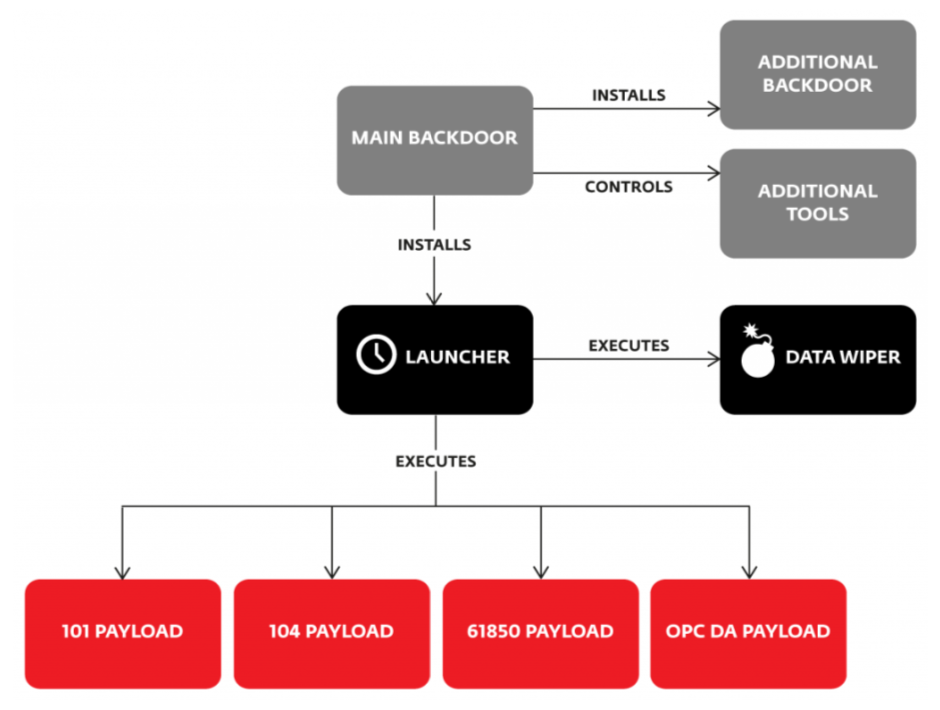
\includegraphics{payload}}
    \caption{Etapy užitočného zaťaženia\cite{IoTSec}}
\label{payload}
\end{figure}
Zadný vchod do systémov celkom priamočiaro spojuje malware so vzdialeným serverom využívajúc HTTPS protokol na zasielanie príkazov od útočníka. Zaujímavé je, že útočníci si môžu nadefinovať špecifickú hodinu, kedy bude tento vchod do systému aktívny, napríklad mimo pracovnej doby. Keď sa vytvorí spojenie so serverom, v {\tt POST} žiadosti sú zaslané jednotlivé údaje\cite{IoTSec}. \par
Je podporovaných niekoľko základných príkazov:
\begin{itemize}
\item 0: spustenie procesu
\item 1: spustenie procesu pod špecifickým užívateľom s patričnými autentizačnými údajmi
\item 2: stiahnutie súboru zo servera
\item 3: zkopírovanie súboru
\item 4: spustenie {\tt shell} príkazu
\item 5: spustenie {\tt shell} príkazu pod špecifickým užívateľom s patričnými autentizačnými údajmi
\item 6: zastavenie
\item 7: zastavenie služby
\item 8: zastavenie služby pod špecifickým užívateľom s patričnými autentizačnými údajmi
\item 9: spustenie služby pod špecifickým užívateľom s patričnými autentizačnými údajmi
\item 10: nahradenie hodnoty registra {\tt image path} pre danú službu
\end{itemize} \par
Pri užitočnom zaťažení komponent protokolu IEC 104 obsahuje konfiguračný súbor pre jednotlivé komponenty IP adresu stanice, cieľový port, ASDU adresu, hodnotu prepínača (zap./vyp.), hodnotu zmeny (0/1) a operáciu (iteračný typ pre IOA: rozsah, sekvenciu alebo posunutie). \par
Po spustení vytvorí vlákno pre každú sekciu staníc definovaných v konfiguračnom súbore. V každom vlákne komunikuje s konkrétnou adresou využívajúc protokol IEC 104. Po vytvorení spojenia s daným zariadením začne zasielať príkazy s ASDU adresou definovanou v súbore kde interaguje s IOA využívajúc SCO (Single command) typ\cite{IoTSec}. \par
Iteračné typy IOA:
\begin{itemize}
\item Rozsah - využívajúc mód rozsahu môže útočník odhaliť všetky dostupné IOA v cielenom zariadení. Protokol IEC 104 štandardne neposkytuje žiadnu obdobnú metódu na získanie takých údajov. \par 
Keď útočník získa potrebný rozsah IOA, môže cez ne začať iterovať a zasielať príkazy {\tt select and execute}, aby mohol zmeniť typ daného IOA a potvrdiť, že patrí do typu SCO. \par
Keď je preiterované cez všetky potrebné IOA, malware začne rozposielať príkazy {\tt select and execute} v nekonečnom cykle, kde postupne zapína a vypína zariadenia.
\item Sekvencia - tento mód môže byť použitý jedine ak útočník vie hodnoty všetkých IOA, ktoré využívajú SCO typ. Malware môže hneď začať nekonečný cyklus v ktorom bude posielať {\tt select and execute} príkazy IOA definovaným v konfiguračnom súbore.
\item Posunutie - je veľmi podobné módu rozsahu. Iteruje sa cez celý rozsah IOA, kde nový rozsah je vypočítaný pridaním hodnoty posunutia k pôvodnej hodnote rozsahu\cite{IoTSec}.
\end{itemize}
\section{Zhrnutie}
SCADA systémy v súčasnosti čelia mnohým rizikám. Je to veľký problém najmä z dôvodu, že systémy sú väčšinou súčasťou kritickej infraštruktúry a útoky na ne môžu mať veľký dopad aj na bežných obyvateľov alebo ekosystém ako taký. Je preto potrebné vedieť útoky včas detekovať a vedieť sa im efektívne brániť. \par
V tejto kapitole bol uvedený základný prehľad bezpečnostných rizík na SCADA systémy spolu s popisom jednotlivých typov útokov. Taktiež bolo uvedených niekoľko príkladov zaznamenaných útokov spolu s dôsledkami, ktoré spôsobili. \par
V ďalšej časti mojej práce budem vychádzať z popisu jednotlivých rizík, ktorým SCADA systémy čelia a vytvorím simulačné prostredie na ich testovanie a sledovanie reakcií systému na ne.





  \chapter{Implementácia}
\label{implementacia}
\tab V kapitole \ref{porovnanie} boli uvedené rôzne premyselne využívané programy a nástroje na simuláciu a riadenie prevádzky SCADA systémov. V kapitole \ref{bezpecnost} bola popísaná bezpečnosť týchto systémov spolu s rôznymi typmi útokov, ktoré sú pre ne hrozbou. Z nadobudnutých informácií bolo navrhnuté a implementované simulačné prostredie pre protokoly DLMS/COSEM a IEC 104 na testovanie rôznych typov útokov a sledovanie reakcií systému na ne. V nasledujúcej časti bude podrobne popísaná implementácia prostredia spolu s testovaním. \par
\section{Návrh prostredia}
\tab Prvý návrh prostredia pre protokol DLMS/COSEM spočíval vo vytvorení vlastného objektu za pomoci C++ knižnice od spoločnosti GuruX, ktorý sa pripojí do existujúcej siete a bude slúžiť ako zadný vchod (backdoor) do systému. Útoky tohto typu boli popísané v kapitole \ref{bezpecnost}. Avšak s novo-vytvoreným objektom nechcel program DLMS Director spolupracovať a nebolo možné vykonávať testy. Po komunikácií so spoločnosťou GuruX som zistil, že program nepodporuje komunikáciu so špecifickými objektami a v čase písania tejto práce nebol program aktualizovaný o túto funkcionalitu. \par
Druhý návrh, ktorý bol spoločný pre oba skúmané protokoly (DLMS/COSEM a IEC 104) pozostával z vytvorenia programu, ktorý bude simulovať stranu klienta, a bude serveru zasielať nevalidné alebo zmenené príkazy, a budú sa sledovať reakcie systémov. Komunikáciu program nevytvára, iba ďalej zasiela príkazy z odchytenej a následne zmenenej komunikácie. Výhodou je, že pracuje na štvrtej (transportnej) vrstve TCP/IP modelu a vďaka tomu nemusí rozlišovať, s akým protokolom komunikuje. Iba posiela ďalej príkazy ktoré dostane na vstupe, a čaká na odpoveď. Na obrázku \ref{orig} je ukážka validného prostredia, z ktorého sa vychádzalo pri testovaní zmien v príkazoch, ako je možné vidieť na obrázku \ref{test}. Validácia vzorových systémov preukázala, že programy sú schopné simulovať komunikáciu odpovedajúcu štandardom protokolov a je preto možné ich použiť na testovacie účely a očakávať obdobné reakcie aj od reálnych zariadení.
\begin{figure}[h]
    \centering
    \scalebox{0.7}{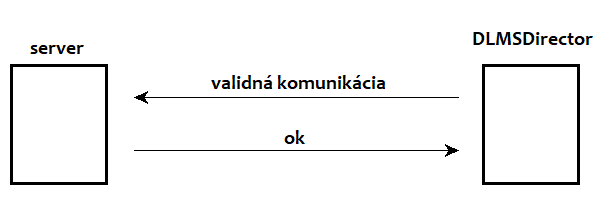
\includegraphics{orig.png}}
    \caption{Vzorový systém}
\label{orig}
\end{figure}
\begin{figure}[h]
    \centering
    \scalebox{0.7}{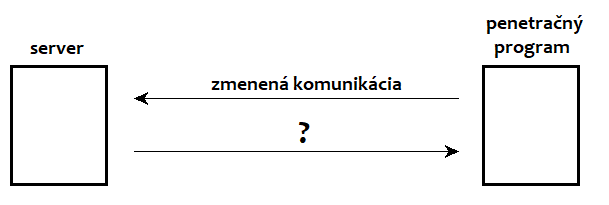
\includegraphics{test.png}}
    \caption{Testovací systém}
\label{test}
\end{figure}
\section{Implementácia simulačného prostredia}
\tab Ako bolo spomenuté vyššie, pre účely simulácie útokov bol vytvorený program klienta, ktorý je schopný zasielať strane servera rôzne zmenené alebo nevalidné príkazy. Program je implementovaný v jazyku C++ a funguje ako TCP klient, ktorý sa pripojí na server. Na vstup dostáva binárny súbor obsahujúci jednotlivé príkazy, ktoré sa budú serveru odosielať. Príkazy boli získané analýzou zachytenej komunikácie medzi reálnymi stanicami klient a server. Analýza prebiehala pomocou nástroja {\tt Wireshark\footnote{Wireshark \url{https://www.wireshark.org}}}. V nástroji bol zobrazený {\tt TCP stream} zachytenej komunikácie a následne odfiltrovaný iba na správy zasielané stranou klienta. Analýza však nemusí prebiehať výhradne pomocou nástroja {\tt Wireshark}. Je možné použiť akýkoľvek obdobný nástroj. Napríklad pre analýzu priamo z príkazovej riadky je možné použiť nástroj {\tt tshark\footnote{TShark \url{https://www.wireshark.org/docs/man-pages/tshark.html}}}, príkazom {\tt tshark -r input.pcap -q -z follow,tcp,raw,0 > output}. Príkaz zobrazí do zadaného súboru binárnu podobu zachytenej komunikácie, ktorú je možné ďalej upravovať. \par
Odfiltrované príkazy boli uložené do binárneho súboru, ktorý sa ďalej posiela ako vstup simulačnému programu. Vďaka tomu, že program pracuje priamo s binárnou podobou príkazov, je možné ich ľubovolne upraviť, a vytvárať so serverom neštandardnú komunikáciu. Odchytenú komunikáciu je možné ďalej analyzovať a zisťovať reakcie systému na rôzne typy útokov. \par
Pri načítavaní jednotlivých príkazov zo súboru je potrebné, aby boli od seba oddelené špecifikým znakom, aby program rozoznal koniec jedného a začiatok druhého. Pôvodne bola zvolená hexadecimálna hodnota {\tt 0x0a}, čo je hodnota pre nový riadok. Túto hodnotu však bolo nutné zmeniť, pretože {\tt 0x0a} sa v jednotlivých príkazoch často vyskytuje aj ako hodnota 10 označujúca objekt alebo namerané dáta. Pri načítavaní to spôsobovalo rozdelenie jedného príkazu na dva. Po tomto zistení som sa pokúšal nájsť inú hexadecimálnu hodnotu ktorá sa nevyskytuje v príkazoch ani jedného z protokolov. Spoločnú hodnotu sa mi nepodarilo nájsť a preto za príkazy protokolu DLMS bola pridaná hodnota {\tt 0x3f} a za príkazy protokolu IEC 104 hodnota {\tt 0x7e}. Príkazy boli upravované v nástroji {\tt Sublime Text 3\footnote{Sublime Text \url{https://www.sublimetext.com}}} po zobrazení hexadecimálneho kódovania. \par 
\subsection{Popis behu programu}
\tab Program pri spustení načíta vstupné argumenty, skontroluje správnosť ich kombinácie a validitu zadaných hodnôt. Keď je všetko v poriadku, zo vstupu sa načítajú jednotlivé príkazy, ktoré sa budú odosielať. Pri spustení programu je potrebné zadať, s akým protokolom má program pracovať, DLMS alebo IEC 104. Je to nutné z dôvodu, že program rozlišuje podľa akého znaku má jednotlivé príkazy od seba odlíšiť, ako už bolo spomínané vyššie. Protokol DLMS/COSEM taktiež využíva na prenos príkazov protokol HDLC, ktorý slúži na spoľahlivý prenos dát po sieti. Súčasťou dátového rámca protokolu sú dva byty vyhradené na tzv. kontrolný súčet CCITT-CRC16. Ukážka rámca je na obrázku \ref{hdlc}. Príkazy protokolu DLMS obsahujú prvý a posledný byte režijný, označujúci začiatok a koniec príkazu, hodnota je {\tt 0x7e}. Následuje adresa, typ príkazu, samotné data a dva byty s hodnotou spomínaného kontrolného súčtu. 
\begin{figure}[h]
    \centering
    \scalebox{0.5}{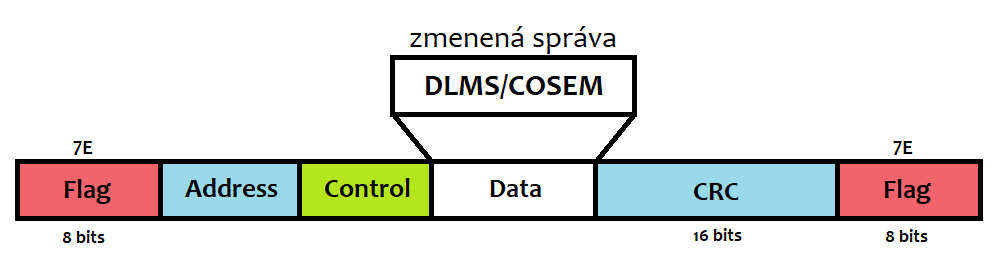
\includegraphics{hdlc.png}}
    \caption{HDLC zapúzdrenie}
\label{hdlc}
\end{figure}
Pre každý zmenený príkaz je potrebné nanovo vypočítať jeho kontrolný súčet. Ten sa počíta z celého rámca, okrem prvého a posledného (režijného bytu). Ak by totiž súčet nesúhlasil s dátami, strana príjemcu (servera) by správu zahodila a prestala by ďalej komunikovať. Implementácia funkcií na výpočet súčtu bola prevzatá zo stránok {\tt stackoverflow.com}\footnote{Stackoverflow \url{https://stackoverflow.com/questions/7983862/calculating-fcscrc-for-hdlc-frame} [Online: Marec 2018]} a {\tt www.zorc.breitbandkatze.de}\footnote{CRC \url{http://www.zorc.breitbandkatze.de/crc.html} [Online: Marec 2018]}. Program načítava jednotlivé príkazy do pomocnej premennej {\tt message} typu {\tt std::vector<std::string>}. Do premennej {\tt answer}, ktorá je rovnakého typu sa ukladajú odpovede od servera. \par
Po načítaní jednotlivých príkazov sa vytvorí TCP spojenie a začína komunikácia. Príkazy sa odosielajú v cykle. Pre protokol DLMS sa vždy odošle jeden príkaz a očakáva sa jedna odpoveď, nakoľko protokol komunikuje synchrónne. Protokol IEC104 je o niečo komplikovanejší. Oproti protokolu DLMS, kde ide o synchrónnu komunikáciu 1:1 (jedna správa : jedna odpoveď), to tak pri protokole IEC 104 nefunguje, komunikácia prebieha asynchrónne. Niekedy je potrebné odoslať niekoľko správ bez odpovedi, alebo očakávať niekoľko odpovedí po jednej správe. Problém bol vyriešený využitím funkcie {\tt select()} spolu s {\tt timeoutom}. Funkcia je volaná v cykle. Ak sa podarí prijať správu, cyklus prijímania sa opakuje, ak vyprší timeout, z cyklu sa vyskočí a odosiela sa nová správa.
Komunikácia je implementovaná pomocou {\tt bsd schránok}. Odosielanie a prijímanie správ zabezpečujú funkcie {\tt send()} a {\tt recv()}. 
\subsection{Návod na použitie}
\subsubsection{Preloženie a spustenie programu}
Program je nutné pred prvým spustením preložiť príkazom {\tt make} v koreňovom adresári projektu. Keď je program preložený, môžeme ho spustiť. Spúšťa sa nasledovným príkazom: \newline
{\tt ./client [-h] [a <adresa serveru>] [-p port] [-i vstupný súbor] [-o výstupný súbor] [--dlms] [--iec]}
\subsubsection{Parametre programu}
Program {\tt client} je možné spustiť s niekoľkými parametrami:
\begin{description}
\item {\tt -h \textendash\textendash help} - zobrazí nápovedu
\item {\tt -a \textendash\textendash address} - IP adresa serveru, s ktorým bude klient komunikovať
\item {\tt -p \textendash\textendash port} - port, na ktorom komunikuje server
\item {\tt -i \textendash\textendash input} - vstupný binárny súbor s jednotlivými príkazmi
\item {\tt -o \textendash\textendash output} - súbor, kam sa budú ukladať odpovede od serveru
\item {\tt -1 \textendash\textendash iec} - komunikácia s iec 104 serverom
\item {\tt -2 \textendash\textendash dlms} - komunikácia s dlms serverom
\end{description}
Vždy musí byť zadaný aspoň jeden z parametrov {\tt -h \textendash\textendash help}, {\tt -a \textendash\textendash address} | {\tt \textendash\textendash dlms}, {\tt -o \textendash\textendash output}. Nemôžu byť zadané oba naraz, ani z jednej kombinácie. Navyše parameter {\tt -h \textendash\textendash help} nemôže byť kombinovaný so žiadnym ďalším parametrom. Pri absencií parametra {\tt -p \textendash\textendash port} sa nastaví predvolená hodnota podľa zadaného protokolu. {\tt 2404} pre IEC 104 a {\tt 4059} pre DLMS. V prípade nezadanie parametrov {\tt -i \textendash\textendash input} a {\tt -o \textendash\textendash output} sa využije štandardný vstup a výstup.
\subsubsection{Príklady použitia}
\begin{description}
\item {\tt ./client -h} - vypíše nápovedu
\item {\tt ./client -a 192.168.137.189 -p 4060 \textendash\textendash dlms -i data1 -o output1} - program bude komunikovať s DLMS serverom na porte 4060 pomocou protokolu TCP. Príkazy si načíta zo súboru {\tt data1} a odpovede od servera zapíše do súboru {\tt output1}. Ak takýto súbor neexistuje, vytvorí ho.
\end{description}
\section{Testovanie}
\tab Pri validácií programu klienta a simulačného prostredia ako takého boli využívané zachytené komunikácie medzi jednotlivými simulátormi SCADA prevádzky. Zachytená komunikácia bola v simulačnom prostredí opätovne vytvorená a zachytená. Po overení, že všetky dvojice komunikácií sú totožné, bol program prehlásený za validný. \par
\begin{figure}[h]
    \centering
    \scalebox{0.5}{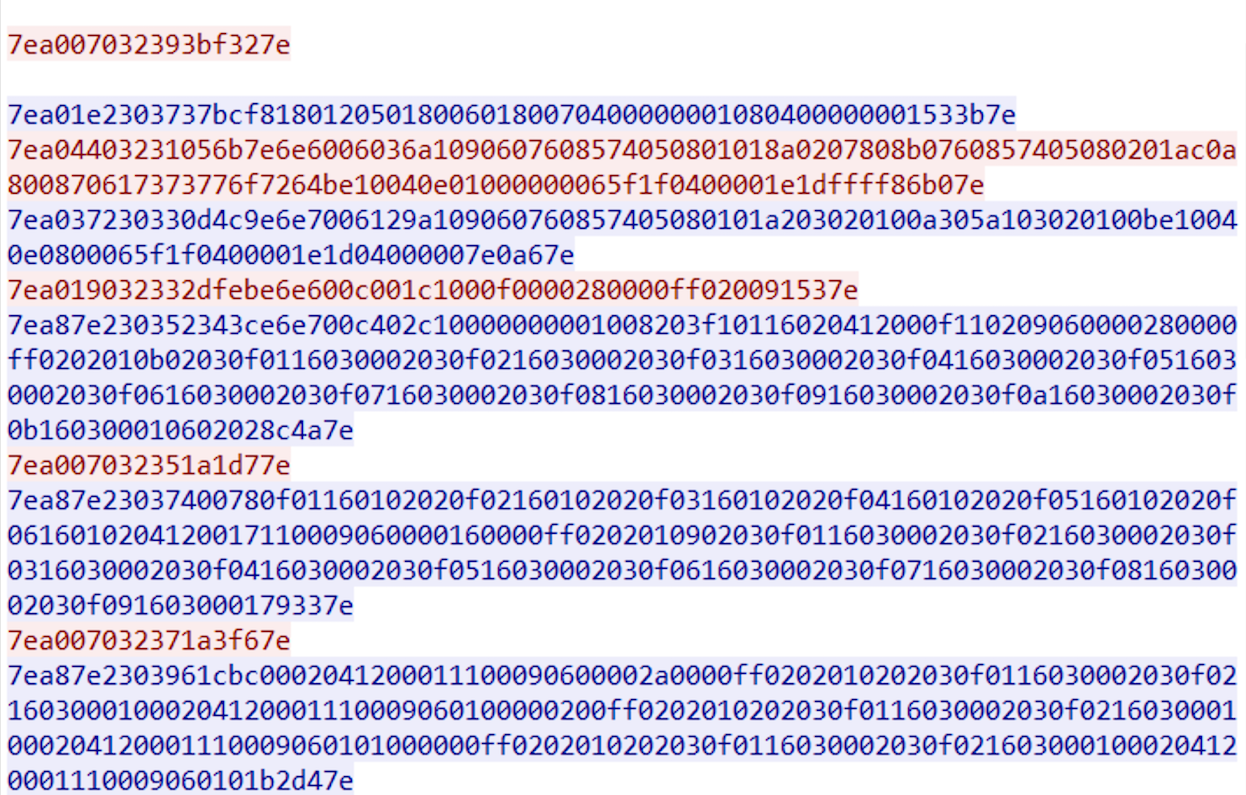
\includegraphics{original}}
    \caption{Originálna komunikácia medzi klientom a serverom}
    \label{original}
\end{figure}
Na obrázku \ref{original} je ukážka časti zachytenej originálnej komunikácie medzi simulačnými nástrojmi pre klienta a server, konkrétne ide o protokol DLMS/COSEM. Na obrázku \ref{testing} je možné vidieť tú istú komunikáciu vygenerovanú pomocou simulačného programu klienta. Obe komunikácie boli následne porovnané programom {\tt diffchecker\footnote{Diffchecker \url{https://www.diffchecker.com} [Online: Marec 2018]}} a bolo overené, že komunikácie sú totožné. \par
\begin{figure}[h]
    \centering
    \scalebox{0.5}{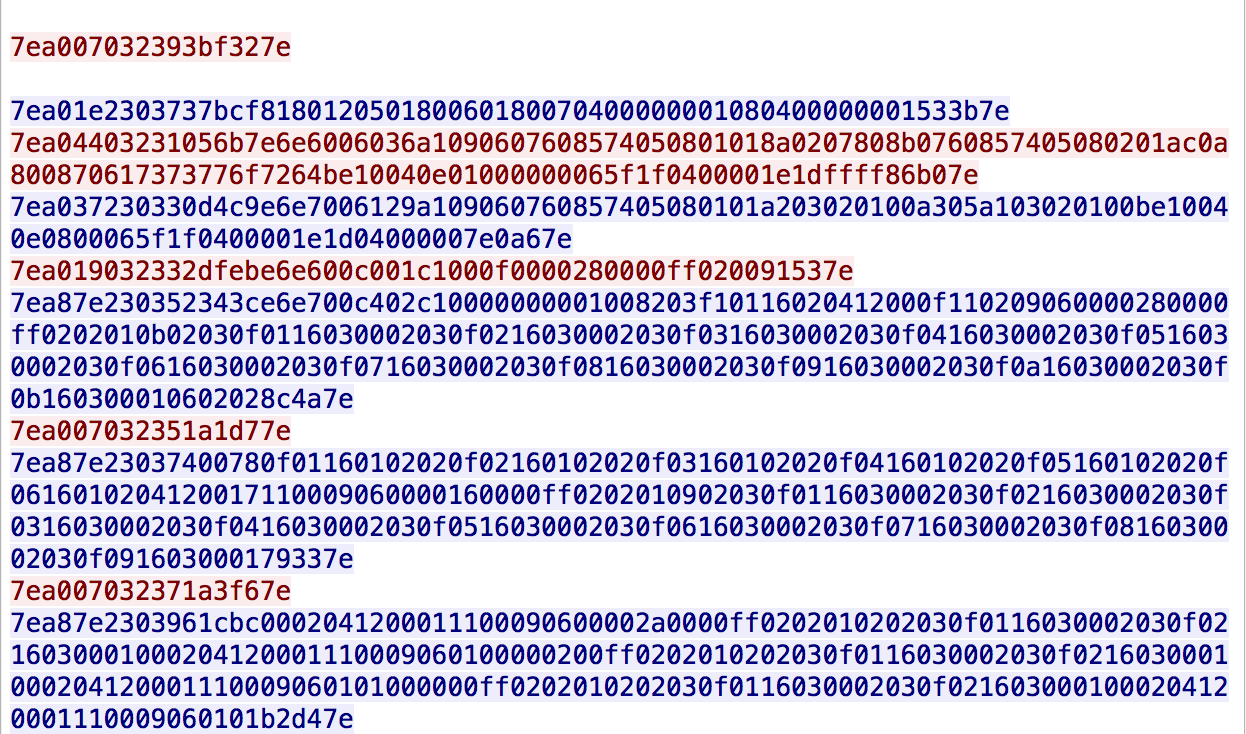
\includegraphics{testing}}
    \caption{Opätovne vygenerovaná komunikácia pomocou programu klienta}
    \label{testing}
\end{figure}
Pri testovaní protokolov bola vždy vytvorená testovacia topológia so vzorovou komunikáciou. Komunikácia bola pri každom teste čiastočne zmenená a boli sledované reakcie systému, ako je možné vidieť na obrázku \ref{monitoring}. \par
\begin{figure}[h]
    \centering
    \scalebox{0.8}{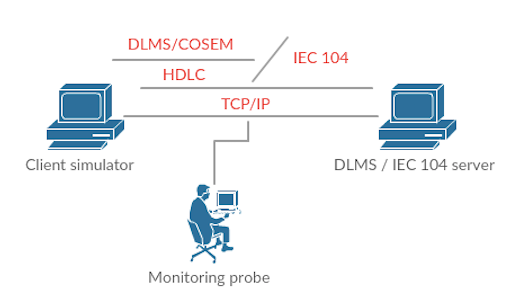
\includegraphics{monitoring}}
    \caption{Sledovanie reakcií systému zo zachytenej komunikácie}
    \label{monitoring}
\end{figure}
Pri testovaní bezpečnostných incidentov na systémy komunikujúce pomocou protokolov DLMS/COSEM a IEC 104 som postupoval v niekoľkých krokoch:
\begin{enumerate}
\item Vytvorenie simulačného prostredia, ktoré sa chová ako reálny systém.
\item Vygenerovanie validnej komunikácie, ktorá bude slúžiť ako vzorová.
\item Pozmenenie príkazov z ochytenej vzorovej komunikácie.
\item Opätovné vygenerovanie s patričnými zmenami.
\item Sledovanie reakcií systému.
\end{enumerate}

\subsection{DLMS/COSEM}
\tab Pri testovaní protokolu DLMS bola využívaná open source knižnica pre jazyk C++ poskytovaná spoločnosťou GuruX. Knižnica je voľne dostupná v Github repozitári\footnote{DLMS knižnica - Github \url{https://github.com/Gurux/Gurux.DLMS.cpp} [Online: Marec 2018]}. Podrobná inštalácia knižnice je popísaná medzi prílohami v časti \ref{kniznica}. Knižnica obsahuje vzorový program pre server, ktorý bol následné upravený pre potreby testovania. Pôvodná implementácia zahŕňa štyry rôzne typy DLMS serverov, pričom každý komunikuje na inom porte. \par
Pri testovaní bol ponechaný iba jeden server využívajúci logické mená (Logical Names), komunikujúci na porte 4060. Taktiež bola povolená možnosť hodnoty v atribútoch jednotlivých objektov aj nastavovať. Pôvodne ich bolo možné iba vzdialene čítať. Čo sa týka knižnice samotnej, implementácia dátových objektov nepodporovala dynamickú zmenu nameraných hodnôt za behu programu. Aby to viac odpovedalo reálnemu systému, v súbore {\tt GXDLMSData.cpp} bola zmenená implementácia {\tt CGXDLMSData::GetValue} metódy, ktorá vracala nameranú hodnotu. Do metódy bola pridaná podmienka, ktorá vráti novú hodnotu ak od predošlého dotazu uplynulo aspoň 10 sekúnd. Uplynutý čas od posledného dotazu sa počíta pomocou premennej typu {\tt std::time\_t}, pričom sa počíta rozdiel jej hodnoty (od posledného dotazu) k aktuálnemu času {\tt std::time(nullptr)}. Nové hodnoty sa získavajú dvoma spôsobmi. Sú generované náhodne funkciou {\tt rand()} alebo sú načítavané zo súboru. Voľba konkrétneho spôsobu je na základe konfiguračného súboru, ktorý je uložený v {\tt Gurux.DLMS.cpp-master/conf}. Obsah konfiguračného súboru môže byť napríklad:
\begin{itemize}
\item {\tt file = ../../values} - nastavenie čítania zo súboru {\tt values} spolu s cestou k nemu
\item {\tt rand = 1000} - nastavenie náhodného generovania hodnôt z rozsahu 0..1000
\end{itemize} \par
\begin{figure}[h]
    \centering
    \scalebox{0.4}{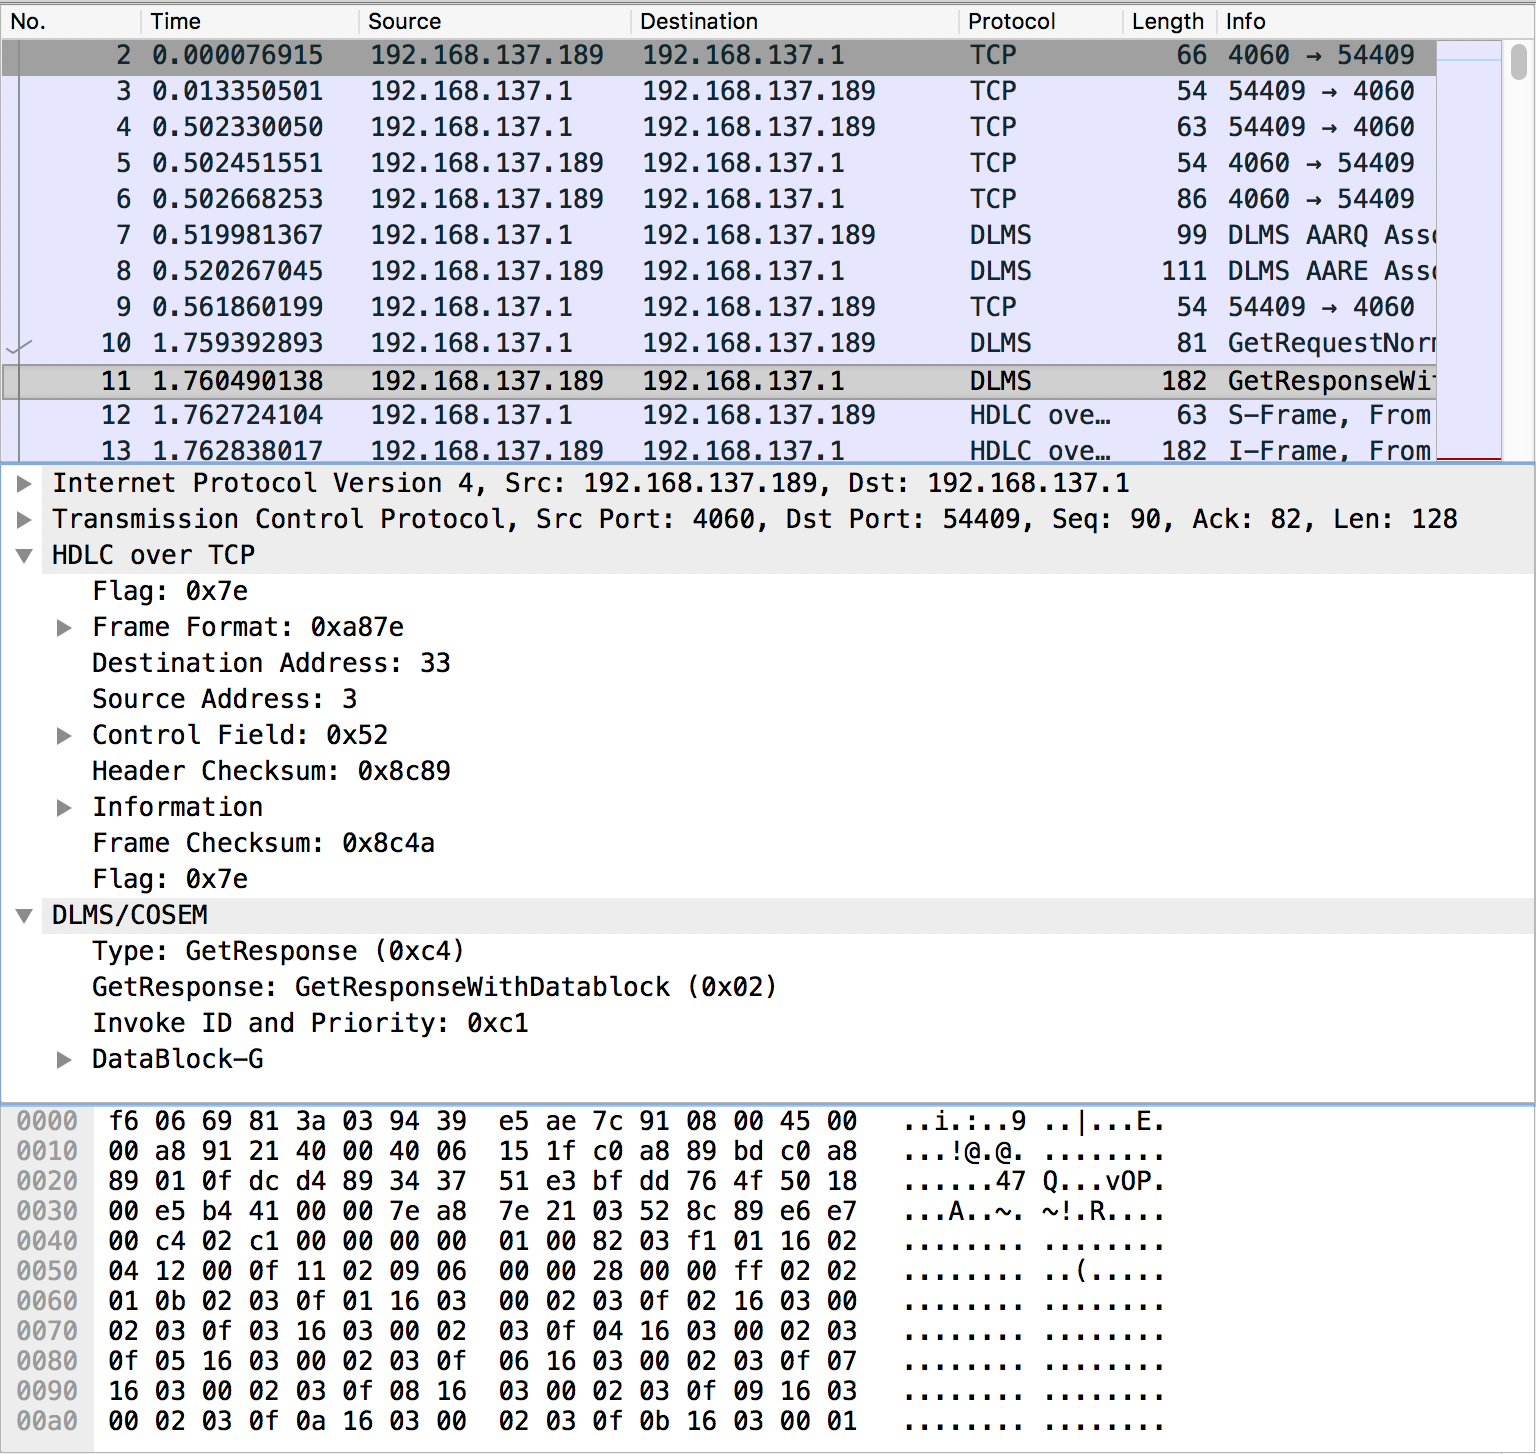
\includegraphics{dissector}}
    \caption{Analýza zachytenej komunikácie}
    \label{dissector}
\end{figure}
Pri analýze zachytených .pcap súborov bol použitý dissector pre program Wireshark vytvorený pánom Ing. Petrom Matouškom, Ph.D., M.A.\footnote{DLMS Dissector \url{https://github.com/matousp/dlms-analysis} [Online: Apríl 2018]} Dissector z načítanej binárnej postupnosti vyberie časti pre HDLC zapúzdrenie a pre samotné dáta protokolu DLMS/COSEM. Ukážku je možné vidieť na obrázku \ref{dissector}.
\subsubsection{Testy}
\subsubsection{Validná komunikácia:} 
Na začiatku testovania bol vytvorený vzorový .pcap súbor obsahujúci validnú (vzorovú) komunikáciu protokolu DLMS/COSEM. Zasielané príkazy boli následne systematicky menené a boli sledované reakcie systému. \par
\noindent \textbf{Zachytenie komunikácie:} dlms.pcap
\subsubsection{Test č. 1:}
\textbf{Zmena:} Data obsahovali zlú veľkosť pri otváraní asociácie v príkaze {\tt AARQ - Association Request}. 11 bytov namiesto 9 bytov: 0x09 $\rightarrow$ 0x0b. \newline
\textbf{Reakcia:} Server si zmenu vôbec nevšímal a zaslal spätne potvrdzovaciu správu o zistení deviatich pripojených zariadení. \par
\noindent \textbf{Zachytenie komunikácie:} data1.pcap
\subsubsection{Test č. 2:}
\textbf{Zmena:} Dĺžka OID prvého požiadavku bola zle zadaná v príkaze {\tt AARQ - Association Request}. 9 bytov namiesto 7 bytov: 0x07 $\rightarrow$ 0x09. \newline
\textbf{Reakcia:} Server si opäť zmenu nevšimol. Žiadosť o asociáciu prijal a odpoveď obsahovala OID zmenené na správne. \par
\noindent \textbf{Zachytenie komunikácie:} data2.pcap
\subsubsection{Test č. 3:}
\textbf{Zmena:} Dĺžka OID prvého požiadavku bola zle zadaná v príkaze {\tt AARQ - Association Request}. 3 byty namiesto 7 bytov: 0x07 $\rightarrow$ 0x03. \newline
\textbf{Reakcia:} Reakcia bola rovnaká ako pri predchádzajúcom teste. \par
\noindent \textbf{Zachytenie komunikácie:} data3.pcap
\subsubsection{Test č. 4:}
\textbf{Zmena:} Zlý typ paketu. Pôvodná správa bola typu {\tt Get-Request} a bola následne zmenená na {\tt Set\--Request}: 0xc0 $\rightarrow$ 0xc1. Zmena bola vykonaná iba v poli obsahujúcom typ. Zvyšok paketu ostal pôvodný pre {\tt Get-Request}. \newline
\textbf{Reakcia:} Server prijal žiadosť na nastavenie hodnoty, vykonal zmenu a odpovedal potvrdzovacou správou o úspešnom nastavení. \par
\noindent \textbf{Zachytenie komunikácie:} data4.pcap
\subsubsection{Test č. 5:}
\textbf{Zmena:} Zlý typ paketu. Namiesto {\tt Get-Request} sa poslalo {\tt Set-Response}: 0xc0 $\rightarrow$ 0xc5. \newline
\textbf{Reakcia:} Server nevedel, ako má zareagovať a na správu neodpovedal. \par
\noindent \textbf{Zachytenie komunikácie:} data5.pcap
\subsubsection{Test č. 6:}
\textbf{Zmena:} Chybný OBIS kód požadovaného objektu. Požaduje sa 0.0.40.0.0.1 namiesto 0.0.40.0.0.255: 0xff $\rightarrow$ 0x01. \newline
\textbf{Reakcia:} Server žiadosť prijal a pokúsil sa vrátiť požadovanú odpoveď. Odoslal ale prázdnu správu, nakoľko požadovaný objekt nepoznal. \par
\noindent \textbf{Zachytenie komunikácie:} data6.pcap
\subsubsection{Test č. 7:}
\textbf{Zmena:} Zmena požadovaného atribútu objektu. Požaduje sa atribút 10 namiesto 1: 0x02 $\rightarrow$ 0x0a. \newline
\textbf{Reakcia:} Server na zmenu reagoval štandardnou odpoveďou a vrátil hodnotu požadovaného atribútu. Tento test bol zameraný skôr na typ útoku, kedy útočník zachytí prebiehajúcu komunikáciu, čiastočne zmení obsah príkazu, ale ponechá ho validný a pošle pô\-vod\-né\-mu adresátovi. Server správu príjme a odpovie, ale riadiacej stanici príde iná odpoveď akú požadovala. Ak nie je odpoveď dostatočne overená, že je to naozaj tá, ktorá bola očakávaná, môže to znamenať napríklad zlú informovanosť o nameraných hodnotách. \par
\noindent \textbf{Zachytenie komunikácie:} data7.pcap
\subsubsection{Test č. 8:}
\textbf{Zmena:} Zasielané správy odpovedali správam z testovacej komunikácie pre protokol DLMSDirector (DLMSDirector.pcap). Test sa zameriaval na sledovanie otvorenia spojenia a testovanie autentizácie. Komunikácia bola analyzovaná v nástroji {\tt Wireshark}, kde bolo sledované v akej podobe sa prenášajú autentizačné údaje po sieti. \newline
\textbf{Reakcia:} Testovanie autentizácie bolo zamerané hlavne na sledovanie prebiehajúcej komunikácie. Bolo overené, že autentizačné kľúče sa prenášajú v otvorenej podobe. Útočník si tak môže jednoducho ochytiť komunikáciu, prečítať si kľúč a vytvoriť svoje vlastné spojenie so systémom. \par
\noindent \textbf{Zachytenie komunikácie:} auth.pcap \newline \par
Testovanie preukázalo, že server sa pokúša na príkaz vždy odpovedať nehľadiac na to, či požadovaný objekt alebo atribút pozná. Spojenie ukončuje iba v prípade nevalidného príkazu. Veľmi nebezpečný je tiež nešifrovaný prenos hesla po sieti, čo umožňuje útočníkom jednoduchý prístup k autentizačným údajom systému.
\subsection{IEC 104}
\tab Pri testovaní protokolu IEC 104 bol využívaný program QTester 104 a IEC 60870-5-104 Server Simulator. Testovacia topológia pozostávala z jedného klienta a jedného servera, ku ktorému bolo pripojených päť objektov typu {\tt Measured Short Float}. Objekty slúžia na ukladanie nameraných hodnôt s pohyblivou rádovou čiarkou. Testovaciu topológiu je možné vidieť na obrázku \ref{iec-testing}.
\begin{figure}[h]
    \centering
    \scalebox{0.8}{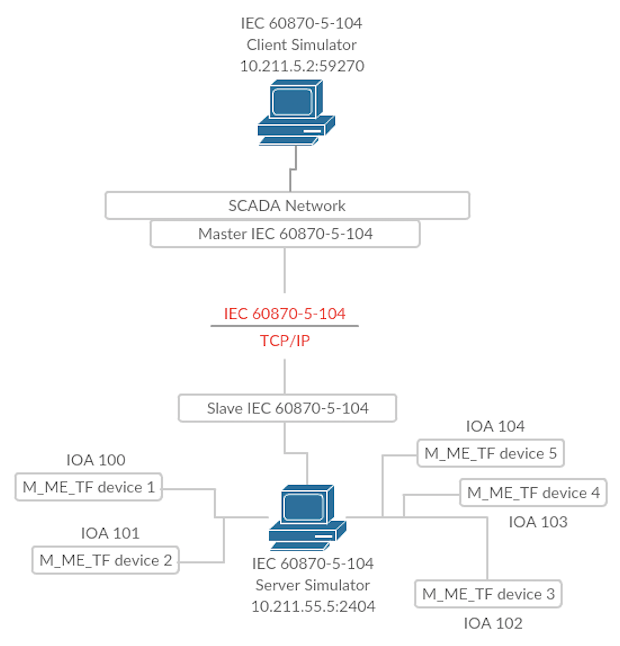
\includegraphics{iec-testing}}
    \caption{Testovacia topológia pre protokol IEC 104}
\label{iec-testing}
\end{figure}
Testovanie protokolu IEC 104 bolo o niečo náročnejšie ako pri protokole DLMS/COSEM z niekoľkých dôvodov. Simulačné programy neumožňovali pridať automatizáciu zmien nameraných hodnôt, a tak bolo potrebné všetky zmeny vykonávať ručne. Z rovnakého dôvodu simulačné prostredie neodpovedalo reálnemu systému do takej miery ako pri DLMS/COSEM. Asynchrónny charakter protokolu tiež trochu skomplikoval opätovné generovanie komunikácie z už odchytenej, ako bolo spomínané vyššie. Posledný problém, ktorý som mal oproti protokolu DLMS/COSEM, bol, že nebolo možné pridať autentizáciu na server a preto ju nebolo možné ani testovať.
\subsubsection{Testy}
\subsubsection{Validná komunikácia:} 
Na začiatku testovania bol vytvorený vzorový .pcap súbor obsahujúci validnú (vzorovú) komunikáciu protokolu IEC 104. Zasielané príkazy boli následne systematicky menené a boli sledované reakcie systému. \par
\noindent \textbf{Zachytenie komunikácie:} iec104.pcap
\subsubsection{Test č. 1:}
\textbf{Zmena:} Test na buffer overflow. Pri nastavovaní hodnoty príkazom {\tt Set point command} bola v poli {\tt Value} zmenená hodnota z 2 na NaN: 0x40 $\rightarrow$ 0xff ffff fff. \newline
\textbf{Reakcia:} Hodnota bola nad rámec povoleného maxima a spôsobila, že dĺžka príkazu bola väčšia ako je štandard, čo spôsobilo, že príkaz bol nevalidný. Server odpovedal hláškou {\tt ERR prefix 1 bytes} spolu s informáciou, že hodnota bola nastavovaná na {\tt nan - Not-A-Number} hodnotu. \par
\noindent \textbf{Zachytenie komunikácie:} data\_buffer\_overflow.pcap
\subsubsection{Test č. 2:}
\textbf{Zmena:} Test na zmenu adresy objektu. Pri nastavovaní hodnoty príkazom {\tt Set point command} bola v poli {\tt Addr} zmenená hodnota adresy cieleného objektu z 1 na 65281: 0x0100 $\rightarrow$ 0x01ff. \newline
\textbf{Reakcia:} Server si zmenu všimol a nevedel nájsť dotazovaný objekt. Odpovedal správou {\tt UkComAdrASDU\_NEGA}. \par
\noindent \textbf{Zachytenie komunikácie:} data\_wrong\_addr.pcap
\subsubsection{Test č. 3:}
\textbf{Zmena:} Test na zmenu dôvodu prenosu. Pri nastavovaní hodnoty príkazom {\tt Set point command} bola v poli {\tt CauseTx} zmenená hodnota z 6 na 10: 0x06 $\rightarrow$ 0x0a (Act (6) na ActTerm (10)). \newline
\textbf{Reakcia:} Server si zmenu všimol a odpovedal správou {\tt UkCauseTx\_NEGA}. \par
\noindent \textbf{Zachytenie komunikácie:} data\_wrong\_cause.pcap
\subsubsection{Test č. 4:}
\textbf{Zmena:} Test na zmenu IOA adresy. Pri nastavovaní hodnoty príkazom {\tt Set point command} bola v poli {\tt IOA} zmenená hodnota z 11 na 15: 0x0b $\rightarrow$ 0x0f. \newline
\textbf{Reakcia:} Server si zmenu všimol a dotazovaný objekt nepoznal. Odpovedal správou {\tt UkIOA\_NEGA}. \par
\noindent \textbf{Zachytenie komunikácie:} data\_wrong\_ioa15.pcap
\subsubsection{Test č. 5:}
\textbf{Zmena:} Test na zmenu OA adresy. Pri nastavovaní hodnoty príkazom {\tt Set point command} bola v poli {\tt OA} zmenená hodnota z 2 na 5: 0x02 $\rightarrow$ 0x05. \newline
\textbf{Reakcia:} Server si zmenu nevšímal a odpovedal potvrdzovacou správou o úspešnom nastavení hodnoty. \par
\noindent \textbf{Zachytenie komunikácie:} data\_wrong\_oa.pcap
\subsubsection{Test č. 6:}
\textbf{Zmena:} Test na zmenu typu id príkazu. Pôvodný príkaz na nastavenie hodnoty - {\tt Set point command} typu {\tt C\_SE\_NC\_1} bol zmenený na typ {\tt C\_BO\_NA\_1 - Bitstring of 32 bits}. Zmena bola vykonaná v poli {\tt TypeId} z hodnoty 50 na hodnotu 51: 0x32 $\rightarrow$ 0x33. Zvyšok príkazu zostal pôvodný pre príkaz typu {\tt C\_SE\_NC\_1}. \newline
\textbf{Reakcia:} Server si zmenu všimol a odpovedal správou {\tt UkIOA\_NEGA}. \par
\noindent \textbf{Zachytenie komunikácie:} data\_wrong\_type\_id.pcap
\subsubsection{Test č. 7:}
\textbf{Zmena:} Posledný test bol opäť nameraný na zmenu hodnoty IOA adresy. Pri nastavovaní hodnoty príkazom {\tt Set point command} bola v poli {\tt IOA} zmenená hodnota z 11 na 12: 0x0b $\rightarrow$ 0x0c. \newline
\textbf{Reakcia:} Server zmenu prijal, cielený objekt našiel medzi pripojenými a odpovedal potvrdzovacou správou o úspešnom nastavení hodnoty. \par
\noindent \textbf{Zachytenie komunikácie:} different\_ioa.pcap \newline










  \chapter{Detekcia útokov na SCADA systémy}
\tab V nasledujúcej kapitole sa zameriam na možnosti detekcie rôznych typov útokov popísaných v kapitole \ref{bezpecnost} spolu s popisom ochrany systémov a sietí pred nimi. \par
Na obrázku \ref{attack} je možné vidieť model jednoduchého kybernetického útoku.
\begin{figure}[h]
    \centering
    \scalebox{0.7}{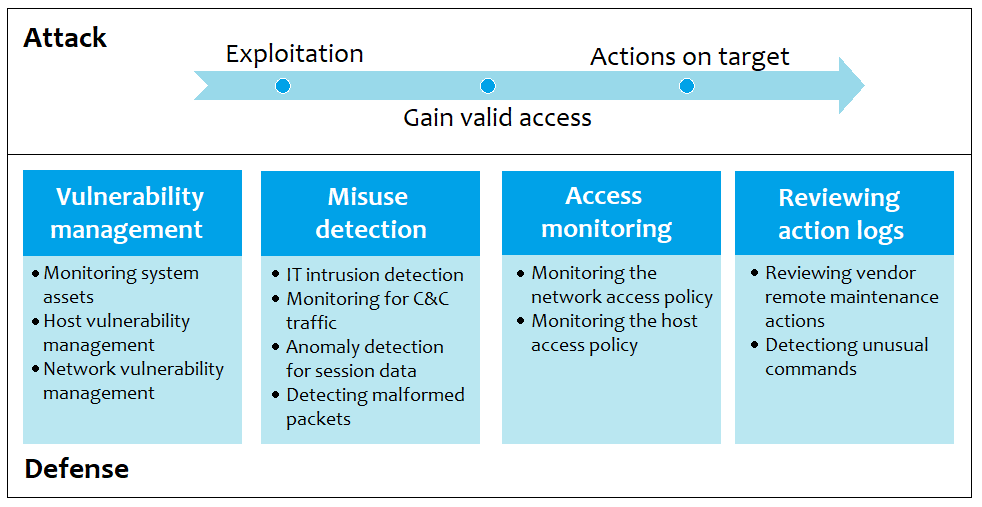
\includegraphics{attack}}
    \caption{Model jednoduchého kyber-útoku}
\label{attack}
\end{figure}
Myšlienka za týmto modelom je, že väčšina útokov začína s využitím zraniteľností danej siete kvôli získaniu prístupu do systému. Keď sa raz útočník dostane "dnu", snaží sa získať oprávnenia na získanie platného prístupu k jednotlivým prvkom systému. Akonáhle má čo potreboval, vykoná kroky potrebné na dosiahnutie svojho cieľa, napríklad na prepnutie alebo vypnutie rôznych častí siete. \par
Stratégia detekcie pozostáva zo štyroch častí:
\begin{itemize}
\item Kontrola a riadenie zraniteľností systému - nájdenie a odstránenie zraniteľných miest skôr ako môžu byť využité útočníkom.
\item Detekcia zneužitia - detekovanie napadnutia systému.
\item Monitorovanie prístupu - detekovanie neoprávnených alebo škodlivých akcií s platnými povereniami.
\item Kontrola logovacích záznamov - zisťovanie akcií s platnými povereniami, ktoré sú škodlivé alebo proti bezpečnostným pravidlám.
\end{itemize}
Model na obrázku \ref{attack} je veľmi zjednodušený. Skutočný útok nemusí byť takto priamočiarý. Útočníci môžu napríklad potrebovať nájsť niekoľko zraniteľných miest v systéme, kým sa im ich podarí využiť a získať platný prístup. Môžu tiež vykonávať rôzne akcie na preskúmanie vlastností danej siete alebo môžu úplne preskočiť fázu hľadania zraniteľných miest, ak už majú k dispozícií platne autentizačné údaje\cite{Security}\cite{IoTSec}.

\section{Kontrola a riadenie zraniteľností systému}
\tab Aktivity kontroly a riadenia zraniteľností sú iba preventívne opatrenia pre systém. Pokúšajú sa nájsť a opraviť zraniteľné miesta a zadné vchody (backdoor) do systému, skôr ako sú odhalené útočníkmi. Ako také zmierňujú väčšinu hrozieb s výnimkou vnútorných, ktoré sa využívajú iba s platnými povereniami. \par
Sú zamerané na hľadanie chýb v systéme a na ich opravu. V OT sieťach je zabezpečenie veľmi závislé od architektúry daného systému. Ak sa v sieti využívajú staršie zariadenia, je potrebné hľadať zraniteľné miesta priamo v architektúre, nakoľko nie je možné sa spoliehať iba na zabezpečenie daného zariadenia. \par
Na efektívnu kontrolu je potrebné mať podrobný prehľad o pripojených zariadeniach a o ich konfigurácií. Tieto informácie uľahčujú nájsť a opravit slabé miesta a zadné vchody do systému. Základné aktivity na kontrolu systému sú:
\begin{itemize}
\item Sledovať/reagovať na novo-pripojené zariadenia do siete
\item Monitorovať prístupy k portom a MAC adresy na jednotlivých prepínačoch
\item Použiť alarm pri pripojení nového zariadenia
\item Odstrániť neautorizovaných hostov
\end{itemize}
Alarmy na nové zariadenia môžu byť využívané za pomoci aktívneho alebo pasívneho skenovania siete. Aktívne skenovanie môže byť vykonávané za pomoci nástrojov ako {\tt nmap} a pasívne sledovaním sieťovej prevádzky. \par
Avšak vykonávanie takejto aktivity vyžaduje zoznam povolených zariadení, ktoré majú oprávnenie sa pripojiť do SCADA systému, aby mohli byť neoprávnené jednoduchšie detekovateľné. Na začiatku monitorovania ale väčšinou obdobný zoznam nie je plne k dispozícií a tak je potrebné aby sa postupne vytváral spolu s monitorovacou aktivitou. \par
Okrem zoznamu je tiež potrebné dodržiavať isté pravidlá pri pripájaní nového zariadenia. To môže byť riešené podrobným registračným procesom, ktorý pomože analytikom overiť, že zariadenie má oprávnenie na vstup do systému\cite{Security}.

\section{Detekcia zneužitia}
\tab Aktivity na detekovanie zneužitia hľadajú v komunikácií znaky známych útokov. V IT sfére bolo za týmto účelom vyvinutých veľa senzorov a sónd. Môžu byť naviazané na hostiteľa, ako napríklad rôzne antivírové programy, alebo priamo na sieť, ako napríklad rôzne systémy na detekciu narušenia siete. \par
Pôvodne boli senzory využívané na detekciu správnosti autentizačných údajov a podpisov. Používané pravidlá boli spisované priamo výrobcom daného senzoru na základe poznatkov o zaznamenaných útokoch. Na dosiahnutie spoľahlivej úrovne detekcie boli potrebné desaťtisíce pravidiel, ktoré museli byť pravidelne aktualizované. Moderné systémy na detekciu narušení doplňujú tento prístup o využitie inteligentných algoritmov, pomocou ktorých je možné odhaliť niekoľko rôznych tried útokov. Ide o IDS (Intrusion Detection System)/IPS (Intrusion Prevention System) zariadenia, ktoré sa bežne využívajú na detekciu podozrivých aktivít v systéme. \par
Aktivity detekcie zneužitia aktívne hľadajú znaky známych útokov alebo porušenia pravidiel systému. Toto môže byť vykonávané pomocou detekčných systémov naviazaných na hostiteľa alebo na sieť samotnú. Tradične to bolo riešené pomocou znakov útoku (užitočné zaťaženie, porušenie pravidiel), ktoré spustili určitú preddefinovanú udalosť detekčného systému. Moderné systémy využívajú o niečo sofistikovanejšie postupy. Štandardné monitorovanie ich komunikácie sa tiež považuje za časť detekčného postupu, nakoľko sa priamo hľadajú útoky, namiesto odchýlok od bežnej komunikácie, ako to robia systémy na detekciu anomálií. \par
Za účelom detekcie znakov útokov v IT sfére bolo vyvinutých mnoho rôznych senzorov a zariadení, ako napríklad rôzne antivírové programy, systémy na detekciu prieniku ap. Kedže sú OT systémy stále viac a viac založené na IT technológiach ako je TCP/IP prenos, využívanie operačných systémov na báze UNIXu, využívanie webových rozhraní ap., tak sa stali tiež zraniteľnými voči útokom vyvinutým pre IT a je možné pre ne využívať pôvodné detekčné IT senzory. \par
Pri samotnom detekovaní dostávajú analytici rôzne alarmy od jednotlivých senzorov, ktoré musia postupne overovať čo daný alarm spôsobilo a či bola daná aktivita relevantná útoku. \par
Detekčné systémy neustále hľadajú špecifické znaky útokov a tak musia byť stále údržiavané aktuálne kvôli neustále sa meniacej inteligencií útokov. To môže byť vykonávané pomocou automatických aktualizácií a rozširovaní systému o nové znaky útokov\cite{Security}.

\section{Monitorovanie prístupu}
\tab Väčšina systémov, ktoré implementujú kontrolu prístupu taktiež uchovávajú logovacie záznamy o úspešných a neúspešných pokusoch o vstup (prihlásenie) do systému. Monitorovanie takéhoto typu informácií môže pomôcť detekovať veľa rôznych útokov. Monitorovanie kontroly prístupu je v OT systémoch pravdepodobne oveľa dôležitejšie ako v IT systémoch, nakoľko sú OT systémy relatívne otvorené. Ak sa útočníkovi podarí získať platné autentizačné údaje, môže sa voľne pohybovať po systéme a vykonávať validné zmeny. Napríklad kybernetické útoky na Ukrajine využívali iba zraniteľnosti IT sietí, v OT sieťach bolo všetko vykonané s platnými povereniami. Toto je pravdepodobne najjednoduchšia cesta do SCADA systémov, kým nebude bezpečnosť a overovanie autentizácie výrazne zlepšené. \par
Monitorovanie je však efektívne iba vtedy, ak je v systéme jasne daná a dodržiavaná prístupová politika. Jednotlivé procesy by mali mať nadefinované, ktorí užívatelia majú právo na vstup do systému a spúšťanie operácií. Navyše by sa mali presne dodržiavať rôzne rozvrhy na údržbu a aktualizáciu systému, aby analytici vedeli, kto môže kedy pristupovať do systému. \par
Bez takýchto pravidiel a rozvrhov môžu byť analýzy vykonávané iba na základe hrubých heuristík, ako je napríklad hľadanie prístupu do systému v neobvyklých hodinách alebo mnoho po sebe neúspešných pokusov o prihlásenie. Analýza možného incidentu by tak mohla trvať oveľa dlhšie. \par
V SCADA systémoch by mala byť komunikácia a prístupy do siete obzvlášť dôkladne monitorované. Taktiež by mali byť vytvorené pravidlá o povolenom prístupe k jednotlivým sieťovým službám a používaným komunikačným protokolom. Monitorovanie prístupu je jedna z variánt ako tieto pravidlá presadzovať. Je to obzvlášť dôležité pri službách, ktoré nepoužívaniu overovanie autentizáciou. \par
Monitorovanie prístupu a dodržiavanie jednotlivých pravidiel nie je užitočné iba pre bezpečnosť. Môže tiež zlepšiť robustnosť siete tým, že zachytí jej nesprávne konfigurácie. Napríklad ak je nesprávne nakonfigurovaná ip adresa pre sieťové servery ako DNS, SNMP alebo NTP. \par
Najefektívnejší spôsob ako monitorovať prístup do siete je s využitím firewallov, nakoľko sa pomocou nich najlepšie presadzujú prístupové pravidlá. Firewally by mali byť monitorované tak, že sa pravidelne kontrolujú a aktualizujú použité pravidlá, a sledujú sa zachytené upozornenia. Pri monitorovaní by sa mali brať do úvahy všetky firewally v danej doméne:
\begin{itemize}
\item firewally  použité na IT/OT rozhrania
\item firewally použité na poskytovanie vzdialeného prístupu na údržbu
\item firewally použité na spojenie riadiacej stanice s WAN (Wide Area Network) sieťou
\item firewally na koncových staniciach\cite{Security}
\end{itemize}

\section{Kontrola logovacích záznamov}
\tab Kontrola logovacích záznamov znamená analýzu toho, čo všetko bolo v systéme (a so systémom) vykonané. Aplikačný software ako aplikácie pre SCADA systémy udržujú záznamy o operáciach vykonaných jednotlivými užívateľmi. Taktiež môže byť prevádzka v SCADA systéme rozdelená na extrakciu iba špecifických príkazov (záleží od analýzy). Všetky tieto informácie môžu byť použité na nájdenie rôznych príznakov útoku na systém. \par
Aktivity na kontrolu záznamov monitorujú, čo bolo kým v systéme vykonané. Sú definované podľa rôznych skupín užívateľov: dodávatelia, ktorí vykonávajú údržbu koncových zariadení na diaľku, zamestnanci, ktorí vykonávají údržbu v rámci spoločnosti a operátori SCADA systému, ktorí vysielajú príkazy do koncových staníc. Samozrejme, keď útočník získa platné autentizačné údaje z jednej z týchto skupín, má prístup ku všetkým operáciam, ktoré môže daná skupina vykonávať. \par
Pri kontrole vzdialeného prístupu do OT systému by mali byť zavedené jednoznačné pravidlá a na rôzne technické opatrenia (údržba ap.) by mal byť stanovený a dodržiavaný presný harmonogram aby analytici mohli rozpoznať prienik do systému od bežnej (plánovanej) údržby. Avšak stále je tu riziko povoliť externým pracovníkom vstup do kritického systému. Aby bolo toto riziko zredukované, je možné pravideľne sledovať a zhodnocovať ich úkony v systéme. \par
Na detekciu útokov zvnútra je užitočné analyzovať logovacie záznamy obsluhy systému. Vykonané akcie môžu byť zaznamenávané operačným systémom, ktorý ukladá kritické príkazy, alebo príkazy spustené s právami administrátora. Od tohto bodu môžu byť detekované zmeny v systémových konfiguráciach\cite{Security}. \par
Pri monitorovaní a analýze komunikácie v sieti sa taktiež často využíva flow monitorovanie. S tým súvisí aj pojem IPFIX (IP Flow Information Export), ktorý označuje export informácií z flow záznamov. IPFIX je veľmi podobný Netflow v tom zmysle, že umožňuje sieťovým administrátorom zbierať informácie o komunikácií zo smerovačov, prepínačov a z akéhokoľvek zariadenia podporujúceho daný protokol. IPFIX má však oproti Netflow niekoľko výhod. Za prvé, informácie, ktoré by za normálnych okolností boli zasielané nástrojmi Syslog alebo SNMP má IPFIX schopnosť integrovať a exportovať priamo v IPFIX paketoch. Tým sa eliminuje potreba týchto dodatočných služieb na zber dát. To v podstate výrobcom hardvéru umožňuje špecifikovať ID výrobcu a vložiť do flow záznamu akúkoľvek proprietárnu informáciu a vyexportovať ho z kolektoru na ďalšiu analýzu a monitorovanie. IPFIX taktiež povoluje polia o premenlivej dĺžke, čo umožňuje uložiť informácie ako URL adresy, správy, HTTP stanice a pod. Pracuje na porte 4739.




  \chapter{Záver}
\section*{Zhodnotenie práce}
SCADA systémy sú v dnešnej dobe veľmi rozšírené a stále pribúdajú nové spoločnosti, ktoré ich využívajú. Avšak rovnako narastá aj počet útočníkov a hrozba, ktorej musia čeliť. Je preto veľmi potrebné a dôležité vedieť jednotlivé útoky včas detekovať a systém pred nimi chrániť. Táto práca sa zameriava na komunikačné protokoly DLMS/COSEM a IEC 104, ktoré sú využívané najmä v energetických odvetviach priemyslu. \par
Práca môže pomocť pri skúmaní reakcií systému na jednotlivé typy útokov a tiež pri vývoji rôznych typov monitorovacích zariadení a sónd, ktoré budú schopné útoky včas odhaliť pri sledovaní prebiehajúcej komunikácie. Súčasťou práce je zhodnotenie rôznych simulačných nástrojov na prevádzku SCADA systémov využívajúcich komunikačný protokol DLMS/COSEM a IEC 104. Pomocou nástrojov a novo-vytvoreného simulačného programu klienta pre jazyk C++ bolo vytvorené simulačné prostredie, umožňujúce testovať jednotlivé útoky a sledovať reakcie systému na ne. \par
Pri jednotlivých testovaniach bola vždy vytvorená jedna vzorová komunikácia a v nej následne niekoľko zmien (jedna v rámci testu). Výsledky testov a zaznamenaná komunikácia bola porovnávaná so vzorovou a následne bolo vyhodnotené chovanie systému na zmeny. \par
Posledná kapitola práce je venovaná popisu rôznych spôsobov detekcie útokov a prevencie pred nimi.
\section*{Výstup práce}
Výstupom práce sú programy a postup vytvorenia simulačného prostredia na testovanie rôznych typov útokov. Vďaka simulačnému programu klienta, ktorý pracuje na štvrtej (transportnej) vrstve TCP/IP modelu je postup aplikovateľný na širokú škálu komunikačných protokolov pracujúcich nad TCP/IP. Výstupom jednotlivých testovaní je datová sada vo formáte .pcap obsahujúca jednotlivé útoky spolu s popisom reakcií systému na ne. Všetky zdrojové kódy a zachytené komunikácie sú k dispozícií na priloženom médiu a v github repozitári\footnote{Github \url{https://github.com/janpristas/bakalarska-praca}}. \par
Práca bola taktiež prezentovaná na študentskej konferencií Excel@FIT a je súčasťou projektu IRONSTONE\footnote{Projekt Ironstone \url{http://www.fit.vutbr.cz/units/UIFS/grants/index.php.cs?id=1101}} vo fakultnej výzkumnej skupine NES@FIT.

  % Pouzita literatura / Bibliography
  % ----------------------------------------------
\ifslovak
  \makeatletter
  \def\@openbib@code{\addcontentsline{toc}{chapter}{Literatúra}}
  \makeatother
  \bibliographystyle{bib-styles/czechiso}
\else
  \ifczech
    \makeatletter
    \def\@openbib@code{\addcontentsline{toc}{chapter}{Literatura}}
    \makeatother
    \bibliographystyle{bib-styles/czechiso}
  \else 
    \makeatletter
    \def\@openbib@code{\addcontentsline{toc}{chapter}{Bibliography}}
    \makeatother
    \bibliographystyle{bib-styles/englishiso}
  %  \bibliographystyle{alpha}
  \fi
\fi
  \begin{flushleft}
  \bibliography{projekt-20-literatura-bibliography}
  \end{flushleft}

  % vynechani stranky v oboustrannem rezimu
  % Skip the page in the two-sided mode
  \iftwoside
    \cleardoublepage
  \fi

  % Prilohy / Appendices
  % ---------------------------------------------
  \appendix
\ifczech
  \renewcommand{\appendixpagename}{Přílohy}
  \renewcommand{\appendixtocname}{Přílohy}
  \renewcommand{\appendixname}{Příloha}
\fi
\ifslovak
  \renewcommand{\appendixpagename}{Prílohy}
  \renewcommand{\appendixtocname}{Prílohy}
  \renewcommand{\appendixname}{Príloha}
\fi
%  \appendixpage

% vynechani stranky v oboustrannem rezimu
% Skip the page in the two-sided mode
%\iftwoside
%  \cleardoublepage
%\fi
  
\ifslovak
%  \section*{Zoznam príloh}
%  \addcontentsline{toc}{section}{Zoznam príloh}
\else
  \ifczech
%    \section*{Seznam příloh}
%    \addcontentsline{toc}{section}{Seznam příloh}
  \else
%    \section*{List of Appendices}
%    \addcontentsline{toc}{section}{List of Appendices}
  \fi
\fi
  \startcontents[chapters]
  \setlength{\parskip}{0pt}
  % seznam příloh / list of appendices
  % \printcontents[chapters]{l}{0}{\setcounter{tocdepth}{2}}
  
  \ifODSAZ
    \setlength{\parskip}{0.5\bigskipamount}
  \else
    \setlength{\parskip}{0pt}
  \fi
  
  % vynechani stranky v oboustrannem rezimu
  \iftwoside
    \cleardoublepage
  \fi
  \chapter{Inštalácia monitorovacích nástrojov}
\label{Ako}

\tab V tejto kapitole je uvedený popis práce s jednotlivými monitorovacími nástrojmi popísanými v kapitole \ref{porovnanie} Jedná sa o popis, kde jednotlivé nástroje nájsť na internete, postup inštalácie a konfiguráciu koncových zariadení na simuláciu.

\section{DMLS Director}
\label{Ako_DLMS}
\tab Kedže je program DLMS Director typu open source, je možné ho zdarma stiahnuť priamo zo stránky výrobcu\footnote{DLMS Director \url{http://www.gurux.fi/Download} [Online: Október 2017]}. Na stránke je rovnako odkaz na GitHub repozitár v ktorom je možné nájsť zdrojové kódy programu. Po stiahnutí inštalačného súboru, ho stačí spustiť a program sa automaticky nainštaluje. K programu je od výrobcu poskytovaný online manuál \footnote{DLMS Director manuál \url{https://www.gurux.fi/GXDLMSDirectorHelp} [Online: Október 2017]}, ktorý veľmi prehľadne popisuje prácu s programom. Práca s nástrojom je ale aj bez návodu veľmi jednoduchá. Pri pridávaní nového zariadenia postupujeme v niekoľkých krokoch:
\begin{enumerate}
\item Spustiť DLMS Director
\item V DLMS Directore nakonfigurovať server s ktorým sa ide program spojiť:
\begin{enumerate}
\item {\tt File} $\rightarrow$ {\tt Add Device}
\item Zvoliť meno pre server
\item Zvoliť výrobcu $\rightarrow$ {\tt Gurux}, 
\item Zvoliť typ autentizácie a heslo (ak server využíva autentizáciu)
\item Nastaviť IP adresu servera a port
\end{enumerate}
\item Po úspešnom nakonfigurovaní vytvoriť spojenie so serverom. Spojenie inicializuje program DLMS Director. V ľavom paneli je potrebné rozkliknúť zoznam {\tt Devices} a kliknúť pravým tlačítkom na server, následne na {\tt Connect}.
\item Po vytvorení spojenia sa zobrazí zoznam pripojených zariadení, z ktorých je možné čítať a zapisovať hodnoty, príkazy {\tt Read} a {\tt Write}.
\end{enumerate} \par
Na stránke programu je podrobný postup ako nakonfigurovať jednotlivé zariadenia, ktoré k programu pripájame\footnote{DLMS Director konfigurácia \url{http://www.gurux.fi/GXDLMSDirectorExample} [Online: Október 2017]}.

\section{XmlDemo}
\label{Ako_XML}
\tab XmlDemo je zdarma poskytovaný nástroj spoločnosti iCube. Je možné ho opäť stiahnuť na stránke výrobcu\footnote{XmlDemo \url{https://icube.ch/xmldemo/xmldemo.html} [Online: Október 2017]}. Jednotlivé vývojové balíky v ktorých je program napísaný však nie sú voľne k dispozíci. Je ale možné napísať priamo spoločnosti so žiadosťou o ne. Odkaz na inštalačný súbor je na konci vyššie odkazovanej stránky, predtým je celkom podrobný návod ako s programom pracovať, ako pripájať jednotlivé zariadenia, čítať z nich hodnoty a pod. 
Inštalácia prebieha v niekoľkých krokoch:
\begin{enumerate}
\item Spustiť stiahnutý súbor a vyskočí nám sprievodca inštaláciou
\item {\tt Next} $\rightarrow$ Vybrať zložku, kam sa program nainštaluje $\rightarrow$ {\tt Next} $\rightarrow$ {\tt Install}
\item Program sa nainštaluje a môžme ho spustiť
\end{enumerate} \par
Pri pridávaní nového zariadenia postupujeme nasledovane:
\begin{enumerate}
\item Spustiť XmlDemo
\begin{enumerate}
\item {\tt Show} $\rightarrow$ {\tt Settings}
\item {\tt Select profile (TCP/HDLC)}
\item Nastaviť IP adresu servera a port
\item Nastaviť referenčný model a prípadne heslo
\item Nastaviť timeout, obe hodnoty {\tt Connect} a {\tt Response} na prijateľné hodnoty v milisekundách
\item Nastaviť adresy pre klienta aj server
\end{enumerate}
\item Po nakonfigurovaní je možné vytvoriť spojenie. {\tt Do} $\rightarrow$ {\tt Connect} a {\tt Do} $\rightarrow$ {\tt Read object-list}.
\end{enumerate} \par

\section{WinPP104}
\label{Ako_Win}
\tab WinPP104 sa dá stiahnuť na stránke spoločnosti, ktorá program vytvorila\footnote{WinPP104 \url{http://www.ppfink.de//} [Online: Október 2017]}. 
Inštalácia prebieha v niekoľkých krokoch:
\begin{enumerate}
\item Spustiť stiahnutý súbor a vyskočí nám sprievodca inštaláciou
\item Vybrať jazyk inštalácie (angličtina/nemčina) $\rightarrow$ {\tt OK} $\rightarrow$ {\tt Next}
\item Vybrať zložku, kam sa program nainštaluje $\rightarrow$ {\tt Next}
\item Vybrať názov zložky, ktorý sa vytvorí v Štart menu $\rightarrow$ {\tt Next}
\item Zvoliť, či chceme zástupcu na ploche $\rightarrow$ {\tt Next} $\rightarrow$ {\tt Install}
\end{enumerate} \par
Po inštalácií je možné program spustiť. Výrobca k programu tiež poskytuje podrobný manuál ako s programom pracovať\footnote{WinPP104 - manuál \url{http://www.ppfink.de//downloads/Bed104Usa.pdf} [Online: Október 2017]}.

\section{Knižnica OpenMUC - j60870}
\label{Ako_Open}
\tab Knižnica j60870 je na stiahnutie priamo na stránke výrobcu\footnote{j60870 \url{https://www.openmuc.org/iec-60870-5-104/download/} [Online: Október 2017]}. Priamo v stiahnutej zložke sú už dva preložené binárne súbory, v zložke {\tt run-scripts}. Konkrétne sa jedná o jednoduchú aplikáciu klienta a servera. Na aplikáciach je pekne vidieť čo sa dá pomocou knižnice naimplementovať. Ja osobne som ich spúšťal cez terminál. Na spustenie je ale nutné mať nainštalované Java JDK. Čo sa týka samotnej knižnice, stačí ju vložiť do projektu v jazyku Java a ľubovolne s ňou pracovať. Súčasťou je aj rozsiahla dokumentácia popisujúca jednotlivé funkcie, ktoré knižnica ponúka\footnote{Javadoc \url{https://www.openmuc.org/iec-60870-5-104/javadoc/} [Online: Október 2017]}.

\section{QTester 104}
\label{Ako_QT}
\tab Výrobca programu QTester 104 nemá vlastnú stránku produktu. Pre stiahnutie programu je potrebné navštíviť stránku {\tt sourceforge.net}\footnote{QTester 104 \url{https://sourceforge.net/projects/qtester104/} [Online: Október 2017]}. Na stránke nájdete zložku súboru obsahujúcu zdrojové kódy programu (v zložke {\tt src}) a samotný spustitelný súbor (v zložke {\tt bin}). Program nie je nutné inštalovať, stačí ho iba spustiť. Po spustení je možné pripojiť ľubovolné meracie zariadenia komunikujúce cez protokol IEC 60870-5-104. Bohužiaľ výrobca neposkytuje nijaký návod na prácu s programom. Samotné GUI je ale veľmi intuitívne a návod nie je ani potrebný. Pri pripájaní nového servera sa postupuje v niekoľkých krokoch:
\begin{enumerate}
\item Spustiť program QTester 104: {\tt qtester104} $\rightarrow$ {\tt bin} $\rightarrow$ {\tt QTester104}
\item Zadať ip adresu servera
\item Po úspešnom spojení, kliknúť na {\tt GI (General Interrogation)} aby sa načítali objekty pripojené k serveru
\item Zakliknúť {\tt Log Messages}, prípadne {\tt AutoScroll} na zobrazenie logovacej správy
\end{enumerate}

\section{IEC 60870-5-104 Client/Server Simulator}
\label{Ako_IEC}
\tab Programy IEC 60870-5-104 Client a Server Simulator síce majú vlastnú internetovú stránku, ale inštalačné súbory na demoverzie na nej nenájdeme. Aspoň nie priamo. Kvôli inštalačným súborom je nutné vyplniť určité osobné informácie. Spätne nám potom spoločnosť pošle na emailovú adresu, ktorú sme zadali, odkaz na stiahnutie daného programu. Súbory sa dajú stiahnuť aj nepriamo na stránke {\tt sourceforge.net}\footnote{IEC 60870-5-104 Client/Server Simulator \url{https://sourceforge.net/u/freyrscada/profile/} [Online: November 2017]}. Inštalácia oboch programov prebieha rovnako:
\begin{enumerate}
\item Spustiť stiahnutý súbor a vyskočí nám sprievodca inštaláciou
\item {\tt Next} Zobrazia sa licenčné podmienky k danému programu. Po prečítaní klikneme na {\tt I Agree}. Prípadne, ak s podmienkami nesúhlasíme, môžeme inštaláciu zrušiť tlačidlom {\tt Cancel}
\item Po odsúhlasení vyberieme kam sa program nainštaluje $\rightarrow$ {\tt Next}
\item Vybrať názov zložky, ktorý sa vytvorí v Štart menu $\rightarrow$ {\tt Next}
\item Zvoliť, či chceme zástupcu na ploche $\rightarrow$ {\tt Next} $\rightarrow$ {\tt Install}
\end{enumerate} \par

Po úspešnom nainštalovaní môžeme program spustiť a pracovať s ním. Pridávanie nových uzlov (klient, server) prebieha v oboch programoch obdobne:
\begin{enumerate}
\item Spustiť programu klienta/servera
\item Kliknutie na {\tt Add Client/Server}
\item Nastaviť ip adresu a port
\item Pre server je potrebné nastaviť pripojené objekty
\begin{enumerate}
\item {\tt Configuration} $\rightarrow$ {\tt Add Row} $\rightarrow$ pridať požadované objekty
\item {\tt Load Configuration}
\end{enumerate}
\item {\tt Data\_Objects} $\rightarrow$ {\tt Start Communication}
\item Klient sa pripojí k serveru a zobrazí pripojené objekty
\end{enumerate} \par
Uzly sa dajú nastaviť celkom komplexne, vyžaduje to však väčšiu znalosť problematiky. Spoločnosť ale poskytuje veľmi dobre spracované inštruktážne videá na vytvorenie koncových staníc a prácu s nimi. Videá sú štyri a je možné ich nájsť na stránke spoločnosti\footnote{Tutoriály \url{http://freyrscada.com/iec-60870-5-104-Client-Simulator.php} [Online: November 2017]}. So samotnými programami je možné pracovať maximálne 15 minút, nakoľko ide o demoverzie. Po opätovnom spustení je potrebné opäť nastaviť všetky predošlé konfigurácie.

\chapter{Inštalácia C++ knižnice pre protokol DLMS}
\label{kniznica}
Open source C++ knižnicu pre protokol DLMS poskytovanú spoločnosťou GuruX je možné nájsť na stránke Github\footnote{DLMS knižnica - Github \url{https://github.com/Gurux/Gurux.DLMS.cpp} [Online: Marec 2018]}. Koreňová zložka obsahuje časť {\tt development} obsahujúcu všetky komponenty samotnej knižnice. Ďalej sú tam vzorové programy pre klienta a server. Oba v samostatnej zložke. Pre nainštalovanie knižnice je potrebné ísť do zložky {\tt development} a vytvoriť zložky {\tt lib} a {\tt obj}. Potom spustiť priložený {\tt Makefile}. Prekladač ale zahlási niekoľko chýb. Všetky sa týkajú súborov {\tt GXDLMSAssociationLogicalName.h/.cpp}. Súbory obsahujú znaky {\tt >>} a prekladač si pravdepodobne myslí, že má ísť o bitovú operáciu na mieste, kde by byť nemala. Je tam preto potrebné pridať medzeru a prepísať to na {\tt > >}. Teraz keď spustíme {\tt make}, preklad by mal prejsť bez problémov. Pre inštaláciu vzorového klienta a servera je tiež vytvorený {\tt Makefile}. Samostatný pre každý program, vždy v jeho zložke. Pred spustením je opäť potrebné vytvoriť dve nové zložky, tentokrát {\tt bin} a {\tt obj}. Po vytvorení môžeme zadať príkaz {\tt make}.


 % viz. prilohy.tex / see prilohy.tex
\end{document}
